
%--------------- Personalize your document here ---------------

\author{} % Enter your name
\newcommand{\studentID}{} % enter your student ID
\newcommand{\supervisorone}{} % Enter your supervisor's name
\newcommand{\supervisortwo}{}% Leave it empty or enter your second supervisor's name 
\newcommand{\department}{}
\newcommand{\exam}{}

\title{} %Enter the title of your report 
\date{\today} % insert a specific date	

%--------------------------------------------------------------

% This document was adapted from the
% TEMPLATE FOR PHYS250 WORKSHEET created by Alastair McLean
% URL: https://www.overleaf.com/latex/templates/phys250-worksheet-template/xxftvfhmwqdt

% Jefferson Silveira
% Email: 19jdls1@queensu.ca
% Last update: 09-Jun-2021
% If you have any questions or concerns, do not hesitate to contact me.
%--------------------------------------------------------------

\documentclass[twoside,11pt]{article}

\usepackage{jmlr2e}

% Heading arguments are {volume}{year}{pages}{submitted}{published}{author-full-names}

\usepackage[left=30mm,top=30mm,right=30mm,bottom=30mm]{geometry}
\usepackage{etoolbox} %required for cover page
\usepackage{booktabs}
\usepackage[table,xcdraw]{xcolor}
\usepackage[usestackEOL]{stackengine}
\usepackage[T1]{fontenc}
\usepackage[utf8]{inputenc}
\usepackage{bm}
\usepackage{graphicx}
\usepackage{subcaption}
\usepackage{amsmath}
\usepackage{amsfonts}
\usepackage{mathtools}
\usepackage{xcolor}
\usepackage{float}
%\usepackage{hyperref}
%\usepackage[capitalise]{cleveref}
\usepackage{enumitem,kantlipsum}
\usepackage{amssymb}
\usepackage{amsbsy}
\usepackage{amsthm}
\usepackage{bbm}% theorems, definitions, etc.
\usepackage{pifont}
\usepackage{caption}
\usepackage{multirow}
\usepackage[ruled,vlined]{algorithm2e}
\usepackage{listings}
\usepackage{dirtytalk}
\usepackage{graphicx}
\usepackage{chngcntr}
\usepackage{apptools}
\usepackage{mathrsfs}
\usepackage{wrapfig}
\usepackage{makecell}
\usepackage{tikz}
\usetikzlibrary{positioning,shapes,arrows}
%\renewcommand{\listingscaption}{Algorithm}
%\renewcommand{\listoflistingscaption}{List of Algorithms}
\newcommand{\E}{\mathbb{E}}
\newcommand{\R}{\mathbb{R}}
\DeclareMathOperator*{\argmin}{arg\,min}
\DeclareMathOperator*{\argmax}{arg\,max}
\newcommand{\F}{\mathcal{F}}
\newcommand{\M}{ (\mathcal{M}_1, \mathcal{M}_2)}



\usepackage{booktabs}
 \usepackage{multirow}
 \usepackage{tabularx}
 \usepackage{siunitx}
 \usepackage{xcolor,colortbl}
 \usepackage{threeparttable}
 \usepackage{makecell}

 \sisetup{
   table-number-alignment = center,
   detect-weight = true,
   detect-family = true,
   input-ignore = {\,\%},
    table-format=1.2,
 }
 \definecolor{HeaderGray}{gray}{0.98}
 \definecolor{RowAlt}{gray}{0.97}
 \definecolor{Accent}{HTML}{2D6CDF} % gentle blue for highlights

% \usepackage{booktabs}
% \usepackage{siunitx}
% \usepackage{xcolor,colortbl}
% \usepackage{makecell}
% \definecolor{RowAlt}{gray}{0.97}
% \sisetup{
%   table-number-alignment = center,
%   table-format=1.2,
%   detect-weight = true,
%   detect-family = true
% }



\newtheorem{proposition}{Proposition}
\newtheorem{definition}{Definition}

\newtheorem{example}{Example}
\newtheorem{remark}{Remark}
\newtheorem{assumption}{Assumption}
\newtheorem*{assumption*}{Assumption}
\newtheorem{observation}{Observation}
\newtheorem*{terminology}{Terminology}
\newtheorem{consequence}{Consequence}



\newtheorem{innercustomthm}{Theorem}
\newenvironment{customthm}[1]
  {\renewcommand\theinnercustomthm{#1}\innercustomthm}
  {\endinnercustomthm}

\newtheorem{innercustomlem}{Lemma}
\newenvironment{customlem}[1]
  {\renewcommand\theinnercustomlem{#1}\innercustomlem}
  {\endinnercustomlem}


\newtheorem{innercustomprop}{Proposition}
\newenvironment{customprop}[1]
  {\renewcommand\theinnercustomprop{#1}\innercustomprop}
  {\endinnercustomprop}

  
\newtheorem{innercustomexample}{Example}
\newenvironment{customexample}[1]
  {\renewcommand\theinnercustomexample{#1}\innercustomexample}
  {\endinnercustomexample}

  
\newtheorem{innercustomconsequence}{Consequence}
\newenvironment{customconsequence}[1]
  {\renewcommand\theinnercustomconsequence{#1}\innercustomconsequence}
  {\endinnercustomconsequence}
  
  \newtheorem{theorem}{Theorem}
\newtheorem{lemma}{Lemma}
\newtheorem{notation}{Notation}

\def\b#1{{\color{red}\bf #1}}%

\def\lm#1{{\textcolor{purple}{LM: \bf #1}}}

\newenvironment{myproof}{
  \par\medskip\noindent
  \textit{Proof}.
}{
\newline
\rightline{$\qedsymbol$}
}

\newenvironment{hproof}{%
  \renewcommand{\proofname}{Idea of the proof}\proof}{\endproof}

\newcommand\independent{\protect\mathpalette{\protect\independenT}{\perp}}
\newcommand{\indep}{\perp \!\!\! \perp}
\def\independenT#1#2{\mathrel{\rlap{$#1#2$}\mkern2mu{#1#2}}}


\hypersetup{
    colorlinks,
    linkcolor={black},
    citecolor={blue!50!black},
    urlcolor={blue!80!black}
}

\linespread{1}

\graphicspath{{figures/}}	



\begin{document}

\title{Identifiability of causal graphs under non-additive conditionally parametric causal models}

\author{\name Juraj Bodik \email juraj.bodik@unil.ch \\
       \addr HEC\\
       University of Lausanne\\
      Switzerland
       \AND
       \name Valérie Chavez-Demoulin \email valerie.chavez@unil.ch \\
       \addr HEC\\
       University of Lausanne\\
       Switzerland}

\maketitle

\begin{abstract}
Existing approaches to causal discovery often rely on restrictive modeling assumptions that limit their applicability in real-world settings, particularly when data are heavy-tailed or contain a mixture of discrete and continuous variables. Identifiability of causal graphs has been established under several structural models, including linear non-Gaussian models, post-nonlinear models, and location-scale models. However, these frameworks may not capture the diversity of distributions observed in practice. To address this, we introduce Conditionally Parametric Causal Models (CPCM), a flexible class of models where the conditional distribution of the effect, given its cause, belongs to a known parametric family such as Gaussian, Poisson, Gamma, or Pareto. These models are adaptable to a wide range of practical situations, where the cause influences not only the mean but also the variance or tail behavior of the effect. We demonstrate the identifiability of CPCM by leveraging the concept of sufficient statistics. Furthermore, we propose an algorithm for estimating the causal structure from random samples drawn from CPCM. We evaluate the empirical properties of our methodology on various datasets, demonstrating state-of-the-art performance across multiple benchmarks.


\textbf{Keywords:} causal discovery, structural causal models, identifiability, higher moments, exponential family
\end{abstract}
%TC:ignore
%TC:endignore
  
%\listoffigures
%\newpage
%\listoftables
%\newpage
%\listofalgorithms % List of algorithms in pseudocode format
%\newpage
%\listoflistings % List of algorithms in code format
%\newpage


\pagenumbering{arabic}% Arabic page numbers (and reset to 1)

% This is how you can organize your document
\section{Introduction}
\label{introduction}

Having knowledge regarding causal relationships rather than statistical associations enables us to predict the effects of actions that perturb an observed system \citep{TheBookOfWhy}. Determining causal structures is a fundamental problem in numerous scientific fields \citep{Rubin}. However, different data-generating processes can produce the same observational distribution. Observing the system after interventions is a reliable means to identify the causal structure, but in numerous real-life scenarios, interventions can be too expensive, unethical \citep{epidem_application}, or impossible to observe. Hence, estimating the causal structure from observational data has become an important topic.

In the last few decades, much effort has been put into developing a  mathematical background for a ``language'' of causal inference, centered around the structural causal model (SCM) \citep{Pearl_book}. Given a set of random variables $\textbf{X} = (X_1, \dots, X_d)^\top\in\mathbb{R}^d$, a SCM with an underlying acyclic graph $\mathcal{G}$ represents a data-generating process where the variables arise from structural equations 
\begin{equation*}
    X_i=f_i(\textbf{X}_{pa_i}, \varepsilon_i),\,\,\,\,\,\,\,\,\, \,\,\,\,\,\,\,i=1,\dots, d, 
\end{equation*}
where $f_i$ are the causal (link) functions, $pa_i$ represent the parents (direct causes) of $X_i$ in $\mathcal{G}$, and $\varepsilon_i$ are jointly independent noise variables. The fundamental goal of causal discovery is to estimate the causal structure (causal graph $\mathcal{G}$).  It is straightforward to compute the distribution of $\textbf{X}$ if the graph $\mathcal{G}$ and the conditional densities are given. Here, we deal with the opposite problem, where the distribution of $\textbf{X}$ (or a random sample) is given and we want to infer $\mathcal{G}$. This task is typically impossible without strong assumptions on the SCM \citep{Elements_of_Causal_Inference}. 

The existing literature in the field presents numerous methods and corresponding results for causal discovery under various assumptions on the Structural Causal Model (SCM) \citep{ZhangReview}. When observing multiple environments following different interventions, the assumptions can be significantly less restrictive \citep{Peters_invariance, Multiple_contexts_Mooij}. However, if the goal is to uncover causal relationships based solely on an observed random sample, the assumptions become more strict; typically assuming additive noise \citep{Lingam, Peters2014, reviewANMMooij}. This assumption of additivity $X_i = f_i(\textbf{X}_{pa_i}) + \varepsilon_i$ suggests that $\textbf{X}_{pa_i}$ influences only the mean of $X_i$, while the tail, variance, and higher moments remain fixed. This is a strong assumption, as the tail or other characteristics of the random variable can provide different information about the causal structure.

In this paper, we develop a framework where $\textbf{X}_{pa_i}$ can arbitrarily affect the mean, variance, tail, or other characteristics of $X_i$. However, a caution has to be taken because if the model is too general, the causal structure will become unidentifiable, meaning that multiple causal structures could produce the same distribution of $\textbf{X}$.
\begin{example}\label{Gaussian case}
    A useful model that allows an arbitrary effect on the variance as well as on the mean is $X_i\mid \textbf{X}_{pa_i}\sim N\big(\mu(\textbf{X}_{pa_i}), \sigma^2(\textbf{X}_{pa_i})\big)$ for some functions $\mu, \sigma$, in which case the structural equation has the form 
\begin{equation*}\label{prva_gaussian_equation}
X_i =  \mu(\textbf{X}_{pa_i})+ \sigma(\textbf{X}_{pa_i})\, \varepsilon_i, \,\,\,\,\,\,\,\,\,\,\varepsilon_i\text{ is Gaussian.}
\end{equation*}
\end{example}

\begin{example}\label{example_Poisson}
In certain applications, it may be reasonable to assume
$$X_i\mid \textbf{X}_{pa_i}\sim Poisson\big(\theta(\textbf{X}_{pa_i})\big),$$where $\theta$ is a function describing the rate of certain phenomena. Such a model is common in applications when $X_i$ represents a number of events occurring in a certain time period. 
\end{example}

We introduce a causal model (we call it the conditionally parametric causal model or CPCM) where the structural equation has the following form: 
\begin{equation}\label{11}\begin{split}
&X_i=f_i(\textbf{X}_{pa_i}, \varepsilon_i) = F^{-1}\big(\varepsilon_i; \theta(\textbf{X}_{pa_i})\big),\,\,\,\,\,\,\varepsilon_i\sim U(0,1), \\&   
\,\,\,\,\,\,\,\,\,\,\,\,\text{ or equivalently } X_i\mid \textbf{X}_{pa_i}\sim F\big(\theta(\textbf{X}_{pa_i})\big), \end{split}
\end{equation}
where $F$ is a known distribution function with a vector of parameters $\theta(\textbf{X}_{pa_i})$. 

\subsection{Setup and notation}
\label{Setup}

We adapt the usual notation of graphical models  (e.g., \citealp{PCalgorithm}). We consider a DAG (directed acyclic graph) $\mathcal{G}=(V,E)$ with a finite set of vertices (nodes) $V=\{1, \dots, d\}$ and a set of directed edges $E$, and write $pa_i(\mathcal{G})$, $ch_i(\mathcal{G})$ and $an_i(\mathcal{G})$ for parents, children and ancestors of the node $i$, respectively. In addition, we say that the node $i\in V$ is a source node if $pa_j(\mathcal{G})=\emptyset$, notation $i\in Source(\mathcal{G})$. Given a random vector $\textbf{X }= (X_i)_{i\in V}$ over some probability space with distribution $F_\textbf{X}$, we identify the vertices $j \in V$ with the variables $X_j$.  We omit the argument $\mathcal{G}$ if evident from the context.  


We frequently use the concept of an exponential family, which is a class of probability distributions whose probability density function can be expressed as: 
\begin{equation}\label{Exponential family of distributions}
p(x;\theta) = h_1(x)h_2(\theta)e^{\sum_{i=1}^q\theta_iT_i(x)},
\end{equation}
where $h_1, h_2, T_i$ are measurable functions. We call $T_i$ a \textit{sufficient} statistic, $h_1$ a base measure, and $h_2$ a normalizing function. Note that $T_i$ are only unique up to a linear transformation.   Many well-known distribution families belong to the exponential family, including the Gaussian, Poisson, Binomial, and Gamma distributions. We assume that $q$ is minimal in the sense that we cannot write $p(x;\theta)$ using only $q-1$ parameters; see Appendix~\ref{appendix_exponential_family} that provides more information and detailed description. 

We use capital $F$ for distributions and small $p$ for densities. A random variable $Z$ that is uniformly distributed on $(0,1)$ is denoted as $Z\sim U(0,1)$. Support of a random variable $Z$ is denoted as $supp(Z)$.  We denote a random vector $\textbf{X}_S = \{X_s{:}\,\, s\in S\}$ for $S\subseteq V$. 

%The SCM uniquely defines a distribution of $\textbf{X}$ that can be decomposed into a product of conditional densities or causal Markov kernels \citep[Definition 6.21]{Elements_of_Causal_Inference}
%\begin{equation}%\label{def987}
%p_\textbf{X}(\textbf{x}) = \prod_{i\in V} p_i(x_i\mid \textbf{x}_{pa_i}),
%\end{equation}
%where $p_i(\cdot \mid \textbf{x}_{pa_i})$ represents the conditional density function of the random variable $X_i$ conditioned on its parents $\textbf{X}_{pa_j}=\textbf{x}_{pa_j}$. 
%A core concept in causal inference is the identifiability of the causal structure. It is straightforward to compute $F_{\textbf{X}}$ if the underlying DAG and the Markov kernels \eqref{def987} are given. However, we deal with the opposite problem, where $F_{\textbf{X}}$ is given (or a random sample from $F_{\textbf{X}}$) and we want to infer the DAG. This is generally not possible without further assumptions, as we can only identify the Markov equivalence class \citep[Proposition 7.1]{Elements_of_Causal_Inference}. More formal definition of identifiability is provided in Section 3. 

%Consider a SCM with conditional densities that satisfy (\ref{def987}). 
%Let  $\mathcal{G}\in DAG(d)$, where $DAG(d)$ is the set of all DAGs over $V=\{1, \dots, d\}$ and assume that $p_i\in\mathcal{H}_i$, where $\mathcal{H}_i$ is the subset of all conditional density functions. Let $\mathcal{H} = \mathcal{H}_1\times \dots \times \mathcal{H}_d$. The given pair $(\mathcal{G}, p)\in DAG(d)\times \mathcal{H}$ generates the density $p_p(\textbf{x}) = \prod_{i\in V} p_i(x_i\mid \textbf{x}_{pa_i})$.  

%\begin{definition}\label{IdentifiabilityPrvaDefinicia}
%We say that the pair $(\mathcal{G}, p)$ is identifiable in $DAG(d)\times \mathcal{H}$ if there does \textit{not} exist a pair $(\mathcal{G}', p')\in DAG(d)\times \mathcal{H}$,  $\mathcal{G}'\neq \mathcal{G}$, such that $p_p= p_{p'}$. We say that the class $\mathcal{H}$ is identifiable over $DAG(d)$ if every  pair  $(\mathcal{G}, p)\in DAG(d)\times \mathcal{H}$ is identifiable in $DAG(d)\times \mathcal{H}$.  
%\end{definition}

%Without strong restrictions of class $\mathcal{H}$, we cannot obtain the identifiability of $\mathcal{G}$. 


\subsection{Related work}

Many papers address the problem of the identifiability of the causal structure (for a review, see \cite{ZhangReview}). 
\cite{Lingam} show identifiability for the linear non-Gaussian additive models (LiNGaM), where $X_i=\beta\textbf{X}_{pa_i} +\varepsilon_i$ for non-Gaussian noise variables $\varepsilon_i$. 
\cite{BuhlmannCAM} explore causal additive models (CAM) of the form $X_i = \sum_{j\in pa_i} g_j(X_j) +  \varepsilon_i$ for smooth functions $g_j$.  
\cite{hoyer2009} and \cite{Peters2014} develop a framework for additive noise models (ANM), where $X_i = g(\textbf{X}_{pa_i}) +  \varepsilon_i$. Under certain (not too restrictive) conditions on $g$, the authors show the identifiability of such models  \citep[Corollary 31]{Peters2014} and propose an algorithm estimating $\mathcal{G}$ (for a review on ANM, see \cite{reviewANMMooij}). 
All these frameworks assume that the variance of $X_i\mid \textbf{X}_{pa_i}$ does not depend on $\textbf{X}_{pa_i}$. This is a crucial aspect of the identifiability results.

\cite{Zhang2009} introduce a generalization known as the post-nonlinear model, defined by $
X_i = g_1\big(g_2(\textbf{X}_{pa_i}) +  \varepsilon_i\big),
$
with an invertible link function $g_1$.  
 \cite{ParkPoisson, ParkVariance} reveal identifiability in discrete models in which  $var[X_i\mid \textbf{X}_{pa_i}]$  is a quadratic function of $\mathbb{E}[X_i\mid \textbf{X}_{pa_i}]$. If $X_i\mid \textbf{X}_{pa_i}$ has a Poisson or binomial distribution, such a condition is satisfied.  They also provide an algorithm based on comparing dispersions for estimating a DAG in polynomial time. Other algorithms have also been proposed, with comparable speed and different assumptions on the conditional densities \citep{PolynomialTimeAlgorithmCausalGraphs}. \cite{Galanti} consider the neural SCM with representation $X_i = g_1\big(g_2(\textbf{X}_{pa_i}), \varepsilon_i\big),$ where $g_1$ and $g_2$ are assumed to be neural networks. 

Recently, location-scale models of the form 
\( X_i = g_1(\textbf{X}_{pa_i}) +  g_2(\textbf{X}_{pa_i})\varepsilon_i \)
have garnered attention. \cite{immer2022identifiability} demonstrated that bivariate non-identifiable location-scale models must satisfy a specific differential equation. \cite{strobl2022identifying} explored the problem of estimating patient-specific root causes in location-scale models. Additionally, \cite{Khemakhem_autoregressive_flows} provided more detailed identifiability results under Gaussian noise $\varepsilon_i$ in the bivariate case using autoregressive flows. \cite{xu2022inferring} investigated a more restricted location-scale model, dividing the range of the predictor variable into a finite set of bins and fitting an additive model in each bin.

Further, several different algorithms for estimating causal graphs have been proposed, working with different assumptions \citep{IGCI, Score-based_causal_learning, Slope, Natasa_Tagasovska}.  They are often based on Kolmogorov complexity or independence between certain functions in a deterministic scenario. 

Constraint-based methods, like the PC and FCI algorithms \citep{PCalgorithm, FCI}, are considered a gold standard for causal discovery. They utilize sequential independence testing for causal discovery, consistently estimating the Markov equivalence class. While these methods are powerful, they rely heavily on the accuracy of the conditional independence tests, making them sensitive to statistical errors and often resulting in many edges remaining unoriented.

A few authors assume that causal Markov kernels lie in a parametric family of distributions. \cite{JanzingSecondOrderExponentialModels} consider the case in which the density of  $X_i\mid \textbf{X}_{pa_i}$  lies in a second-order exponential family and the variables are a mixture of discrete and continuous random variables. \cite{ParkGHD} concentrate on a specific subclass of model (\ref{11}), where $F$ lies in a discrete family of generalized hypergeometric distributions---that is, the family of random variables in which the mean and variance have a polynomial relationship. To the best of our knowledge, there does not exist any study in the literature, that provides identifiability results in the case in which $F$ lies in a general class of the exponential family. This is the focus of this paper. 

\textbf{The structure of the paper is as follows.} Section \ref{Section2} introduces the main definitions and motivation in a bivariate case. Section \ref{Section_identifiability} presents identifiability results for the causal structure in the bivariate case, and Section \ref{Section4} discusses the multivariate extension. In Section \ref{Section5}, we propose an algorithm for estimating the causal graph under assumption (\ref{11}). Section \ref{simulations_section} contains an extensive simulation study. We provide three appendices: Appendix \ref{Appendix_A} includes formal definition of Exponential family and some omitted technical content; Appendix \ref{Appendix_simulations} details the experiments and Appendix \ref{SectionProofs} contains all proofs.

















































































































\tikzset{every picture/.style={line width=0.75pt}} %set default line width to 0.75pt        

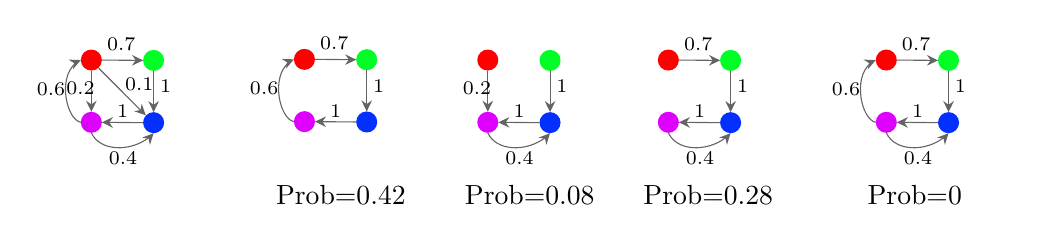
\begin{tikzpicture}[x=0.75pt,y=0.75pt,yscale=-1,xscale=1]
%uncomment if require: \path (0,300); %set diagram left start at 0, and has height of 300

%Shape: Circle [id:dp6680159379724935] 
\draw  [draw opacity=0][fill={rgb, 255:red, 255; green, 0; blue, 0 }  ,fill opacity=1 ] (210,135.27) .. controls (210,132.47) and (212.27,130.2) .. (215.07,130.2) .. controls (217.86,130.2) and (220.13,132.47) .. (220.13,135.27) .. controls (220.13,138.06) and (217.86,140.33) .. (215.07,140.33) .. controls (212.27,140.33) and (210,138.06) .. (210,135.27) -- cycle ;
%Shape: Circle [id:dp2937575833870516] 
\draw  [draw opacity=0][fill={rgb, 255:red, 0; green, 255; blue, 38 }  ,fill opacity=1 ] (240,135.43) .. controls (240,132.64) and (242.27,130.37) .. (245.07,130.37) .. controls (247.86,130.37) and (250.13,132.64) .. (250.13,135.43) .. controls (250.13,138.23) and (247.86,140.5) .. (245.07,140.5) .. controls (242.27,140.5) and (240,138.23) .. (240,135.43) -- cycle ;
%Shape: Circle [id:dp5400820274117357] 
\draw  [draw opacity=0][fill={rgb, 255:red, 3; green, 47; blue, 255 }  ,fill opacity=1 ] (240,165.43) .. controls (240,162.64) and (242.27,160.37) .. (245.07,160.37) .. controls (247.86,160.37) and (250.13,162.64) .. (250.13,165.43) .. controls (250.13,168.23) and (247.86,170.5) .. (245.07,170.5) .. controls (242.27,170.5) and (240,168.23) .. (240,165.43) -- cycle ;
%Shape: Circle [id:dp012766690091095434] 
\draw  [draw opacity=0][fill={rgb, 255:red, 222; green, 0; blue, 255 }  ,fill opacity=1 ] (210,165.27) .. controls (210,162.47) and (212.27,160.2) .. (215.07,160.2) .. controls (217.86,160.2) and (220.13,162.47) .. (220.13,165.27) .. controls (220.13,168.06) and (217.86,170.33) .. (215.07,170.33) .. controls (212.27,170.33) and (210,168.06) .. (210,165.27) -- cycle ;
%Straight Lines [id:da5536414406911649] 
\draw [color={rgb, 255:red, 100; green, 100; blue, 100 }  ,draw opacity=1 ]   (220.13,135.27) -- (237,135.41) ;
\draw [shift={(240,135.43)}, rotate = 180.48] [fill={rgb, 255:red, 100; green, 100; blue, 100 }  ,fill opacity=1 ][line width=0.08]  [draw opacity=0] (5.36,-2.57) -- (0,0) -- (5.36,2.57) -- (3.56,0) -- cycle    ;
%Straight Lines [id:da8056930605061887] 
\draw [color={rgb, 255:red, 100; green, 100; blue, 100 }  ,draw opacity=1 ]   (223.13,165.29) -- (240,165.43) ;
\draw [shift={(220.13,165.27)}, rotate = 0.48] [fill={rgb, 255:red, 100; green, 100; blue, 100 }  ,fill opacity=1 ][line width=0.08]  [draw opacity=0] (5.36,-2.57) -- (0,0) -- (5.36,2.57) -- (3.56,0) -- cycle    ;
%Straight Lines [id:da5796955635821128] 
\draw [color={rgb, 255:red, 100; green, 100; blue, 100 }  ,draw opacity=1 ]   (215.07,140.33) -- (215.07,157.2) ;
\draw [shift={(215.07,160.2)}, rotate = 270] [fill={rgb, 255:red, 100; green, 100; blue, 100 }  ,fill opacity=1 ][line width=0.08]  [draw opacity=0] (5.36,-2.57) -- (0,0) -- (5.36,2.57) -- (3.56,0) -- cycle    ;
%Straight Lines [id:da788839051424455] 
\draw [color={rgb, 255:red, 100; green, 100; blue, 100 }  ,draw opacity=1 ]   (245.07,140.5) -- (245.07,157.37) ;
\draw [shift={(245.07,160.37)}, rotate = 270] [fill={rgb, 255:red, 100; green, 100; blue, 100 }  ,fill opacity=1 ][line width=0.08]  [draw opacity=0] (5.36,-2.57) -- (0,0) -- (5.36,2.57) -- (3.56,0) -- cycle    ;
%Straight Lines [id:da09644761921540357] 
\draw [color={rgb, 255:red, 100; green, 100; blue, 100 }  ,draw opacity=1 ]   (218.63,139.22) -- (239.15,159.76) ;
\draw [shift={(241.27,161.88)}, rotate = 225.04] [fill={rgb, 255:red, 100; green, 100; blue, 100 }  ,fill opacity=1 ][line width=0.08]  [draw opacity=0] (5.36,-2.57) -- (0,0) -- (5.36,2.57) -- (3.56,0) -- cycle    ;
%Curve Lines [id:da6909993804639241] 
\draw [color={rgb, 255:red, 100; green, 100; blue, 100 }  ,draw opacity=1 ]   (207.42,136.86) .. controls (198.7,144.14) and (203.19,163.99) .. (210,165.27) ;
\draw [shift={(210,135.27)}, rotate = 156.35] [fill={rgb, 255:red, 100; green, 100; blue, 100 }  ,fill opacity=1 ][line width=0.08]  [draw opacity=0] (5.36,-2.57) -- (0,0) -- (5.36,2.57) -- (3.56,0) -- cycle    ;
%Curve Lines [id:da43617986234567363] 
\draw [color={rgb, 255:red, 100; green, 100; blue, 100 }  ,draw opacity=1 ]   (215.07,170.33) .. controls (219.24,179.43) and (233.96,179.59) .. (242.88,172.51) ;
\draw [shift={(245.07,170.5)}, rotate = 133.09] [fill={rgb, 255:red, 100; green, 100; blue, 100 }  ,fill opacity=1 ][line width=0.08]  [draw opacity=0] (5.36,-2.57) -- (0,0) -- (5.36,2.57) -- (3.56,0) -- cycle    ;
%Shape: Circle [id:dp9613652888659034] 
\draw  [draw opacity=0][fill={rgb, 255:red, 255; green, 0; blue, 0 }  ,fill opacity=1 ] (312.67,134.93) .. controls (312.67,132.14) and (314.94,129.87) .. (317.73,129.87) .. controls (320.53,129.87) and (322.8,132.14) .. (322.8,134.93) .. controls (322.8,137.73) and (320.53,140) .. (317.73,140) .. controls (314.94,140) and (312.67,137.73) .. (312.67,134.93) -- cycle ;
%Shape: Circle [id:dp4333461787824253] 
\draw  [draw opacity=0][fill={rgb, 255:red, 0; green, 255; blue, 38 }  ,fill opacity=1 ] (342.67,135.1) .. controls (342.67,132.3) and (344.94,130.03) .. (347.73,130.03) .. controls (350.53,130.03) and (352.8,132.3) .. (352.8,135.1) .. controls (352.8,137.9) and (350.53,140.17) .. (347.73,140.17) .. controls (344.94,140.17) and (342.67,137.9) .. (342.67,135.1) -- cycle ;
%Shape: Circle [id:dp03365070392980951] 
\draw  [draw opacity=0][fill={rgb, 255:red, 3; green, 47; blue, 255 }  ,fill opacity=1 ] (342.67,165.1) .. controls (342.67,162.3) and (344.94,160.03) .. (347.73,160.03) .. controls (350.53,160.03) and (352.8,162.3) .. (352.8,165.1) .. controls (352.8,167.9) and (350.53,170.17) .. (347.73,170.17) .. controls (344.94,170.17) and (342.67,167.9) .. (342.67,165.1) -- cycle ;
%Shape: Circle [id:dp9062547154952614] 
\draw  [draw opacity=0][fill={rgb, 255:red, 222; green, 0; blue, 255 }  ,fill opacity=1 ] (312.67,164.93) .. controls (312.67,162.14) and (314.94,159.87) .. (317.73,159.87) .. controls (320.53,159.87) and (322.8,162.14) .. (322.8,164.93) .. controls (322.8,167.73) and (320.53,170) .. (317.73,170) .. controls (314.94,170) and (312.67,167.73) .. (312.67,164.93) -- cycle ;
%Straight Lines [id:da5461621784127331] 
\draw [color={rgb, 255:red, 100; green, 100; blue, 100 }  ,draw opacity=1 ]   (322.8,134.93) -- (339.67,135.07) ;
\draw [shift={(342.67,135.1)}, rotate = 180.48] [fill={rgb, 255:red, 100; green, 100; blue, 100 }  ,fill opacity=1 ][line width=0.08]  [draw opacity=0] (5.36,-2.57) -- (0,0) -- (5.36,2.57) -- (3.56,0) -- cycle    ;
%Straight Lines [id:da09616201897578192] 
\draw [color={rgb, 255:red, 100; green, 100; blue, 100 }  ,draw opacity=1 ]   (325.8,164.96) -- (342.67,165.1) ;
\draw [shift={(322.8,164.93)}, rotate = 0.48] [fill={rgb, 255:red, 100; green, 100; blue, 100 }  ,fill opacity=1 ][line width=0.08]  [draw opacity=0] (5.36,-2.57) -- (0,0) -- (5.36,2.57) -- (3.56,0) -- cycle    ;
%Straight Lines [id:da5502296583487012] 
\draw [color={rgb, 255:red, 100; green, 100; blue, 100 }  ,draw opacity=1 ]   (347.73,140.17) -- (347.73,157.03) ;
\draw [shift={(347.73,160.03)}, rotate = 270] [fill={rgb, 255:red, 100; green, 100; blue, 100 }  ,fill opacity=1 ][line width=0.08]  [draw opacity=0] (5.36,-2.57) -- (0,0) -- (5.36,2.57) -- (3.56,0) -- cycle    ;
%Curve Lines [id:da23324631718484024] 
\draw [color={rgb, 255:red, 100; green, 100; blue, 100 }  ,draw opacity=1 ]   (310.09,136.53) .. controls (301.37,143.81) and (305.86,163.66) .. (312.67,164.93) ;
\draw [shift={(312.67,134.93)}, rotate = 156.35] [fill={rgb, 255:red, 100; green, 100; blue, 100 }  ,fill opacity=1 ][line width=0.08]  [draw opacity=0] (5.36,-2.57) -- (0,0) -- (5.36,2.57) -- (3.56,0) -- cycle    ;
%Shape: Circle [id:dp6818622582337936] 
\draw  [draw opacity=0][fill={rgb, 255:red, 255; green, 0; blue, 0 }  ,fill opacity=1 ] (401,135.27) .. controls (401,132.47) and (403.27,130.2) .. (406.07,130.2) .. controls (408.86,130.2) and (411.13,132.47) .. (411.13,135.27) .. controls (411.13,138.06) and (408.86,140.33) .. (406.07,140.33) .. controls (403.27,140.33) and (401,138.06) .. (401,135.27) -- cycle ;
%Shape: Circle [id:dp06363585140660888] 
\draw  [draw opacity=0][fill={rgb, 255:red, 0; green, 255; blue, 38 }  ,fill opacity=1 ] (431,135.43) .. controls (431,132.64) and (433.27,130.37) .. (436.07,130.37) .. controls (438.86,130.37) and (441.13,132.64) .. (441.13,135.43) .. controls (441.13,138.23) and (438.86,140.5) .. (436.07,140.5) .. controls (433.27,140.5) and (431,138.23) .. (431,135.43) -- cycle ;
%Shape: Circle [id:dp6515401713841082] 
\draw  [draw opacity=0][fill={rgb, 255:red, 3; green, 47; blue, 255 }  ,fill opacity=1 ] (431,165.43) .. controls (431,162.64) and (433.27,160.37) .. (436.07,160.37) .. controls (438.86,160.37) and (441.13,162.64) .. (441.13,165.43) .. controls (441.13,168.23) and (438.86,170.5) .. (436.07,170.5) .. controls (433.27,170.5) and (431,168.23) .. (431,165.43) -- cycle ;
%Shape: Circle [id:dp8403565146161891] 
\draw  [draw opacity=0][fill={rgb, 255:red, 222; green, 0; blue, 255 }  ,fill opacity=1 ] (401,165.27) .. controls (401,162.47) and (403.27,160.2) .. (406.07,160.2) .. controls (408.86,160.2) and (411.13,162.47) .. (411.13,165.27) .. controls (411.13,168.06) and (408.86,170.33) .. (406.07,170.33) .. controls (403.27,170.33) and (401,168.06) .. (401,165.27) -- cycle ;
%Straight Lines [id:da37129508524849975] 
\draw [color={rgb, 255:red, 100; green, 100; blue, 100 }  ,draw opacity=1 ]   (414.13,165.29) -- (431,165.43) ;
\draw [shift={(411.13,165.27)}, rotate = 0.48] [fill={rgb, 255:red, 100; green, 100; blue, 100 }  ,fill opacity=1 ][line width=0.08]  [draw opacity=0] (5.36,-2.57) -- (0,0) -- (5.36,2.57) -- (3.56,0) -- cycle    ;
%Straight Lines [id:da7145815190421096] 
\draw [color={rgb, 255:red, 100; green, 100; blue, 100 }  ,draw opacity=1 ]   (406.07,140.33) -- (406.07,157.2) ;
\draw [shift={(406.07,160.2)}, rotate = 270] [fill={rgb, 255:red, 100; green, 100; blue, 100 }  ,fill opacity=1 ][line width=0.08]  [draw opacity=0] (5.36,-2.57) -- (0,0) -- (5.36,2.57) -- (3.56,0) -- cycle    ;
%Straight Lines [id:da39415211091672386] 
\draw [color={rgb, 255:red, 100; green, 100; blue, 100 }  ,draw opacity=1 ]   (436.07,140.5) -- (436.07,157.37) ;
\draw [shift={(436.07,160.37)}, rotate = 270] [fill={rgb, 255:red, 100; green, 100; blue, 100 }  ,fill opacity=1 ][line width=0.08]  [draw opacity=0] (5.36,-2.57) -- (0,0) -- (5.36,2.57) -- (3.56,0) -- cycle    ;
%Curve Lines [id:da9757843179704913] 
\draw [color={rgb, 255:red, 100; green, 100; blue, 100 }  ,draw opacity=1 ]   (406.07,170.33) .. controls (410.24,179.43) and (424.96,179.59) .. (433.88,172.51) ;
\draw [shift={(436.07,170.5)}, rotate = 133.09] [fill={rgb, 255:red, 100; green, 100; blue, 100 }  ,fill opacity=1 ][line width=0.08]  [draw opacity=0] (5.36,-2.57) -- (0,0) -- (5.36,2.57) -- (3.56,0) -- cycle    ;
%Shape: Circle [id:dp04380357617227837] 
\draw  [draw opacity=0][fill={rgb, 255:red, 255; green, 0; blue, 0 }  ,fill opacity=1 ] (488,135.27) .. controls (488,132.47) and (490.27,130.2) .. (493.07,130.2) .. controls (495.86,130.2) and (498.13,132.47) .. (498.13,135.27) .. controls (498.13,138.06) and (495.86,140.33) .. (493.07,140.33) .. controls (490.27,140.33) and (488,138.06) .. (488,135.27) -- cycle ;
%Shape: Circle [id:dp29949986935781037] 
\draw  [draw opacity=0][fill={rgb, 255:red, 0; green, 255; blue, 38 }  ,fill opacity=1 ] (518,135.43) .. controls (518,132.64) and (520.27,130.37) .. (523.07,130.37) .. controls (525.86,130.37) and (528.13,132.64) .. (528.13,135.43) .. controls (528.13,138.23) and (525.86,140.5) .. (523.07,140.5) .. controls (520.27,140.5) and (518,138.23) .. (518,135.43) -- cycle ;
%Shape: Circle [id:dp5511672247736801] 
\draw  [draw opacity=0][fill={rgb, 255:red, 3; green, 47; blue, 255 }  ,fill opacity=1 ] (518,165.43) .. controls (518,162.64) and (520.27,160.37) .. (523.07,160.37) .. controls (525.86,160.37) and (528.13,162.64) .. (528.13,165.43) .. controls (528.13,168.23) and (525.86,170.5) .. (523.07,170.5) .. controls (520.27,170.5) and (518,168.23) .. (518,165.43) -- cycle ;
%Shape: Circle [id:dp9769153872658556] 
\draw  [draw opacity=0][fill={rgb, 255:red, 222; green, 0; blue, 255 }  ,fill opacity=1 ] (488,165.27) .. controls (488,162.47) and (490.27,160.2) .. (493.07,160.2) .. controls (495.86,160.2) and (498.13,162.47) .. (498.13,165.27) .. controls (498.13,168.06) and (495.86,170.33) .. (493.07,170.33) .. controls (490.27,170.33) and (488,168.06) .. (488,165.27) -- cycle ;
%Straight Lines [id:da5613131489306487] 
\draw [color={rgb, 255:red, 100; green, 100; blue, 100 }  ,draw opacity=1 ]   (498.13,135.27) -- (515,135.41) ;
\draw [shift={(518,135.43)}, rotate = 180.48] [fill={rgb, 255:red, 100; green, 100; blue, 100 }  ,fill opacity=1 ][line width=0.08]  [draw opacity=0] (5.36,-2.57) -- (0,0) -- (5.36,2.57) -- (3.56,0) -- cycle    ;
%Straight Lines [id:da005025679675679795] 
\draw [color={rgb, 255:red, 100; green, 100; blue, 100 }  ,draw opacity=1 ]   (501.13,165.29) -- (518,165.43) ;
\draw [shift={(498.13,165.27)}, rotate = 0.48] [fill={rgb, 255:red, 100; green, 100; blue, 100 }  ,fill opacity=1 ][line width=0.08]  [draw opacity=0] (5.36,-2.57) -- (0,0) -- (5.36,2.57) -- (3.56,0) -- cycle    ;
%Straight Lines [id:da1558253629861852] 
\draw [color={rgb, 255:red, 100; green, 100; blue, 100 }  ,draw opacity=1 ]   (523.07,140.5) -- (523.07,157.37) ;
\draw [shift={(523.07,160.37)}, rotate = 270] [fill={rgb, 255:red, 100; green, 100; blue, 100 }  ,fill opacity=1 ][line width=0.08]  [draw opacity=0] (5.36,-2.57) -- (0,0) -- (5.36,2.57) -- (3.56,0) -- cycle    ;
%Curve Lines [id:da36403543815313033] 
\draw [color={rgb, 255:red, 100; green, 100; blue, 100 }  ,draw opacity=1 ]   (493.07,170.33) .. controls (497.24,179.43) and (511.96,179.59) .. (520.88,172.51) ;
\draw [shift={(523.07,170.5)}, rotate = 133.09] [fill={rgb, 255:red, 100; green, 100; blue, 100 }  ,fill opacity=1 ][line width=0.08]  [draw opacity=0] (5.36,-2.57) -- (0,0) -- (5.36,2.57) -- (3.56,0) -- cycle    ;
%Shape: Circle [id:dp32223667430392] 
\draw  [draw opacity=0][fill={rgb, 255:red, 255; green, 0; blue, 0 }  ,fill opacity=1 ] (593,135.27) .. controls (593,132.47) and (595.27,130.2) .. (598.07,130.2) .. controls (600.86,130.2) and (603.13,132.47) .. (603.13,135.27) .. controls (603.13,138.06) and (600.86,140.33) .. (598.07,140.33) .. controls (595.27,140.33) and (593,138.06) .. (593,135.27) -- cycle ;
%Shape: Circle [id:dp5630106243065429] 
\draw  [draw opacity=0][fill={rgb, 255:red, 0; green, 255; blue, 38 }  ,fill opacity=1 ] (623,135.43) .. controls (623,132.64) and (625.27,130.37) .. (628.07,130.37) .. controls (630.86,130.37) and (633.13,132.64) .. (633.13,135.43) .. controls (633.13,138.23) and (630.86,140.5) .. (628.07,140.5) .. controls (625.27,140.5) and (623,138.23) .. (623,135.43) -- cycle ;
%Shape: Circle [id:dp7466122496388676] 
\draw  [draw opacity=0][fill={rgb, 255:red, 3; green, 47; blue, 255 }  ,fill opacity=1 ] (623,165.43) .. controls (623,162.64) and (625.27,160.37) .. (628.07,160.37) .. controls (630.86,160.37) and (633.13,162.64) .. (633.13,165.43) .. controls (633.13,168.23) and (630.86,170.5) .. (628.07,170.5) .. controls (625.27,170.5) and (623,168.23) .. (623,165.43) -- cycle ;
%Shape: Circle [id:dp031700867746790706] 
\draw  [draw opacity=0][fill={rgb, 255:red, 222; green, 0; blue, 255 }  ,fill opacity=1 ] (593,165.27) .. controls (593,162.47) and (595.27,160.2) .. (598.07,160.2) .. controls (600.86,160.2) and (603.13,162.47) .. (603.13,165.27) .. controls (603.13,168.06) and (600.86,170.33) .. (598.07,170.33) .. controls (595.27,170.33) and (593,168.06) .. (593,165.27) -- cycle ;
%Straight Lines [id:da674567593051244] 
\draw [color={rgb, 255:red, 100; green, 100; blue, 100 }  ,draw opacity=1 ]   (603.13,135.27) -- (620,135.41) ;
\draw [shift={(623,135.43)}, rotate = 180.48] [fill={rgb, 255:red, 100; green, 100; blue, 100 }  ,fill opacity=1 ][line width=0.08]  [draw opacity=0] (5.36,-2.57) -- (0,0) -- (5.36,2.57) -- (3.56,0) -- cycle    ;
%Straight Lines [id:da19529599944373754] 
\draw [color={rgb, 255:red, 100; green, 100; blue, 100 }  ,draw opacity=1 ]   (606.13,165.29) -- (623,165.43) ;
\draw [shift={(603.13,165.27)}, rotate = 0.48] [fill={rgb, 255:red, 100; green, 100; blue, 100 }  ,fill opacity=1 ][line width=0.08]  [draw opacity=0] (5.36,-2.57) -- (0,0) -- (5.36,2.57) -- (3.56,0) -- cycle    ;
%Straight Lines [id:da00219011682676884] 
\draw [color={rgb, 255:red, 100; green, 100; blue, 100 }  ,draw opacity=1 ]   (628.07,140.5) -- (628.07,157.37) ;
\draw [shift={(628.07,160.37)}, rotate = 270] [fill={rgb, 255:red, 100; green, 100; blue, 100 }  ,fill opacity=1 ][line width=0.08]  [draw opacity=0] (5.36,-2.57) -- (0,0) -- (5.36,2.57) -- (3.56,0) -- cycle    ;
%Curve Lines [id:da28811211023069117] 
\draw [color={rgb, 255:red, 100; green, 100; blue, 100 }  ,draw opacity=1 ]   (590.42,136.86) .. controls (581.7,144.14) and (586.19,163.99) .. (593,165.27) ;
\draw [shift={(593,135.27)}, rotate = 156.35] [fill={rgb, 255:red, 100; green, 100; blue, 100 }  ,fill opacity=1 ][line width=0.08]  [draw opacity=0] (5.36,-2.57) -- (0,0) -- (5.36,2.57) -- (3.56,0) -- cycle    ;
%Curve Lines [id:da1762071401291876] 
\draw [color={rgb, 255:red, 100; green, 100; blue, 100 }  ,draw opacity=1 ]   (598.07,170.33) .. controls (602.24,179.43) and (616.96,179.59) .. (625.88,172.51) ;
\draw [shift={(628.07,170.5)}, rotate = 133.09] [fill={rgb, 255:red, 100; green, 100; blue, 100 }  ,fill opacity=1 ][line width=0.08]  [draw opacity=0] (5.36,-2.57) -- (0,0) -- (5.36,2.57) -- (3.56,0) -- cycle    ;

% Text Node
\draw (233.3,127.45) node  [font=\scriptsize] [align=left] {\begin{minipage}[lt]{16pt}\setlength\topsep{0pt}
0.7
\end{minipage}};
% Text Node
\draw (258.83,148.05) node  [font=\scriptsize] [align=left] {\begin{minipage}[lt]{16pt}\setlength\topsep{0pt}
1
\end{minipage}};
% Text Node
\draw (242.03,146.75) node  [font=\scriptsize] [align=left] {\begin{minipage}[lt]{16pt}\setlength\topsep{0pt}
0.1
\end{minipage}};
% Text Node
\draw (213.7,148.75) node  [font=\scriptsize] [align=left] {\begin{minipage}[lt]{16pt}\setlength\topsep{0pt}
0.2
\end{minipage}};
% Text Node
\draw (238.17,160.05) node  [font=\scriptsize] [align=left] {\begin{minipage}[lt]{16pt}\setlength\topsep{0pt}
1
\end{minipage}};
% Text Node
\draw (234.17,182.72) node  [font=\scriptsize] [align=left] {\begin{minipage}[lt]{16pt}\setlength\topsep{0pt}
0.4
\end{minipage}};
% Text Node
\draw (199.5,149.38) node  [font=\scriptsize] [align=left] {\begin{minipage}[lt]{16pt}\setlength\topsep{0pt}
0.6
\end{minipage}};

% Text Node
\draw (335.97,127.12) node  [font=\scriptsize] [align=left] {\begin{minipage}[lt]{16pt}\setlength\topsep{0pt}
0.7
\end{minipage}};
% Text Node
\draw (361.5,147.72) node  [font=\scriptsize] [align=left] {\begin{minipage}[lt]{16pt}\setlength\topsep{0pt}
1
\end{minipage}};
% Text Node
\draw (340.83,159.72) node  [font=\scriptsize] [align=left] {\begin{minipage}[lt]{16pt}\setlength\topsep{0pt}
1
\end{minipage}};
% Text Node
\draw (302.17,149.05) node  [font=\scriptsize] [align=left] {\begin{minipage}[lt]{16pt}\setlength\topsep{0pt}
0.6
\end{minipage}};
% Text Node
\draw (449.83,148.05) node  [font=\scriptsize] [align=left] {\begin{minipage}[lt]{16pt}\setlength\topsep{0pt}
1
\end{minipage}};
% Text Node
\draw (404.7,148.75) node  [font=\scriptsize] [align=left] {\begin{minipage}[lt]{16pt}\setlength\topsep{0pt}
0.2
\end{minipage}};
% Text Node
\draw (429.17,160.05) node  [font=\scriptsize] [align=left] {\begin{minipage}[lt]{16pt}\setlength\topsep{0pt}
1
\end{minipage}};
% Text Node
\draw (425.17,182.72) node  [font=\scriptsize] [align=left] {\begin{minipage}[lt]{16pt}\setlength\topsep{0pt}
0.4
\end{minipage}};
% Text Node
\draw (511.3,127.45) node  [font=\scriptsize] [align=left] {\begin{minipage}[lt]{16pt}\setlength\topsep{0pt}
0.7
\end{minipage}};
% Text Node
\draw (536.83,148.05) node  [font=\scriptsize] [align=left] {\begin{minipage}[lt]{16pt}\setlength\topsep{0pt}
1
\end{minipage}};
% Text Node
\draw (516.17,160.05) node  [font=\scriptsize] [align=left] {\begin{minipage}[lt]{16pt}\setlength\topsep{0pt}
1
\end{minipage}};
% Text Node
\draw (512.17,182.72) node  [font=\scriptsize] [align=left] {\begin{minipage}[lt]{16pt}\setlength\topsep{0pt}
0.4
\end{minipage}};
% Text Node
\draw (616.3,127.45) node  [font=\scriptsize] [align=left] {\begin{minipage}[lt]{16pt}\setlength\topsep{0pt}
0.7
\end{minipage}};
% Text Node
\draw (641.83,148.05) node  [font=\scriptsize] [align=left] {\begin{minipage}[lt]{16pt}\setlength\topsep{0pt}
1
\end{minipage}};
% Text Node
\draw (621.17,160.05) node  [font=\scriptsize] [align=left] {\begin{minipage}[lt]{16pt}\setlength\topsep{0pt}
1
\end{minipage}};
% Text Node
\draw (617.17,182.72) node  [font=\scriptsize] [align=left] {\begin{minipage}[lt]{16pt}\setlength\topsep{0pt}
0.4
\end{minipage}};
% Text Node
\draw (582.5,149.38) node  [font=\scriptsize] [align=left] {\begin{minipage}[lt]{16pt}\setlength\topsep{0pt}
0.6
\end{minipage}};

% Text Node
\draw (237.57,200) node   [align=left] {\begin{minipage}[lt]{20.9pt}\setlength\topsep{0pt}
$\bfpi$
\end{minipage}};


% Text Node
\draw (318,200) node   [align=left] {\begin{minipage}[lt]{20.9pt}\setlength\topsep{0pt}
Prob=0.42
\end{minipage}};


\draw (409,200) node   [align=left] {\begin{minipage}[lt]{20.9pt}\setlength\topsep{0pt}
Prob=0.08
\end{minipage}};


% Text Node
\draw (495,200) node   [align=left] {\begin{minipage}[lt]{20.9pt}\setlength\topsep{0pt}
Prob=0.28
\end{minipage}};

% Text Node
\draw (603,200) node   [align=left] {\begin{minipage}[lt]{20.9pt}\setlength\topsep{0pt}
Prob=0
\end{minipage}};

\end{tikzpicture}

\section{Background}


In this section, we introduce a set of relevant concepts in quantum computing,
% that are  to our work, 
including the building block of quantum computing, the properties of the qubit, and the quantum state of the qubit. 

\def\Zero{
\begin{bmatrix}
    1 \\
    0 \\
\end{bmatrix}}

\def\One{
\begin{bmatrix}
    0 \\
    1 \\
\end{bmatrix}}

\def\sv{
\begin{bmatrix}
    \alpha \\
    \beta \\
\end{bmatrix}}

\def\svcomplex{
\begin{bmatrix}
    a+bi \\
    c+di \\
\end{bmatrix}}


\subsection{Building Block of Quantum Computing}

\textbf{Qubit},
the quantum version of the classic bit, is the basic unit in quantum computing. Similar to a classical bit, there are two computational basis states called state 0 and state 1 for a qubit~\cite{ciaran2021qc4c}. 
However, 
% in contrast to a classical bit, which is either in state 
% 0 or state 1, 
a qubit can also be in an arbitrary linear superposition of state 0 and state 1~\cite{ciaran2021qc4c, rieffel2000introQCnonP}, which is well-known as quantum superposition.
Mathematically, one can represent a qubit using the form of a state vector~\cite{rieffel2000introQCnonP}.
% Bra-Ket Notation or Bloch sphere. 
% Kets like $\ket{x}$ denote column vectors and are typically used to describe quantum states~\cite{rieffel2000introQCnonP}. 
% For instance, state 0 and state 1 can be expressed as $\ket{0}$ = $\Zero$, $\ket{1}$ = $\One$, respectively. 
% When dealing with qubits, and quantum computing in general, a fixed basis with respect to which all statements are made has been chosen in advance. In particular, unless otherwise specified, all measurements will be made concerning the standard basis for quantum computing, ${\ket{0}, \ket{1}}$~\cite{rieffel2000introQCnonP}. 
% As mentioned above, the quantum state $\ket{\psi}$ of a qubit can also be represented in a linear superposition of $\ket{0}$ and $\ket{1}$. 
% Section \ref{qubit_prop} includes more details about the concept of superposition. 

% The state of a single qubit can also be studied by Bloch Sphere. Bloch Sphere is a visual representation of a qubit with similar geometric properties to the unit circle from trigonometry. 
% % Each point on Bloch Sphere corresponds to a different possible superposition of a single qubit~\cite{ciaran2021qc4c}. The top and bottom of the Bloch Sphere correspond to the two measurable quantum states of the qubit, $\ket{0}$ and $\ket{1}$~\cite{ciaran2021qc4c}.
% A vector on the Bloch Sphere, which can point to any of the different locations on the surface of the sphere, indicates the current quantum state of the qubit~\cite{ciaran2021qc4c}. Figure \ref{fig:1}\component{A} is an example of Bloch Sphere visualizing the quantum state of a single qubit. Bloch Sphere is a helpful visualization for understanding how a qubit can have infinite possible quantum states. However, it can only represent one qubit and does not work for systems of two or more qubits~\cite{ciaran2021qc4c, bardin2021microwaves, wie2014bloch}.


% quantum state, superposition, |0>, |1>, psi-matrix, denoted by |0>
% quantum state is represented by |psi>
% similar to classical bit, |0>, |1>
% unlike classical bit, a|0> + b|1>, will discuss this in section 3.2. |psi> = a|0> + b|1> = a[1,0] + b[0,1] = [a,b]


\textbf{Quantum gate},
just like the manipulation of classical bits using classical logic instructions such as \textit{OR} and \textit{AND}, it is applied to qubits to change their quantum states. 
% and the quantum states of qubits change depending on which gate is applied. 
% In Bloch Sphere representation, gates provide instructions for rotating the qubit’s vector around the sphere~\cite{ciaran2021qc4c}. 
Mathematically, quantum gates are represented as operation matrices, acting on single qubit or multiple qubits.
Operations of quantum gates are equivalent to the dot products with the state vector of qubits.
% \yong{Applying xxx to qubits? Please double check the verb.}
% that act on qubits using matrix multiplication.
%Quantum Gate are represented by matrix. Single quantum gate like H, Multiple Quantum gate like CNOT.
%Pics of gate

\textbf{Quantum circuit},
similar to the classical circuit, is the implementation of the quantum program for execution.
A quantum circuit consists of a set of quantum gates, acting on one or multiple fixed qubits.
% in a quantum computer or quantum simulator.
As shown in Figure \ref{fig:case1} and \ref{fig:case2}, a quantum state will be initialized from the start of the quantum circuit and manipulated by quantum gates designed in the quantum circuit. 
% The final execution result is retrieved by measuring each quantum state.




\subsection{Properties of Qubit}
\label{qubit_prop}
\textbf{Superposition}
indicates that a qubit can not only be in one of the computational basis states $\ket{0}$ or $\ket{1}$, but also in a linear superposition of this two states~\cite {nara1999QC4B}.
% As mentioned in Section 3.1, compared with classical bits, the value can only be either 0 or 1, 
Thus, the quantum state $\ket{\psi}$ of a qubit is described by $\alpha\ket{0} + \beta\ket{1}$, where the complex numbers $\alpha$ and $\beta$ are called \textit{amplitudes} such that $|\alpha|^2 + |\beta|^2 = 1$~\cite{rieffel2000introQCnonP}. 
Meanwhile, 
% Once such superposition is measured with respect to the basis state {$\ket{0}$ and $\ket{1}$}, 
the probability of measuring $\ket{0}$ is $|\alpha|^2$ and the probability of $\ket{1}$ is $|\beta|^2$
~\cite{ciaran2021qc4c, rieffel2000introQCnonP,nara1999QC4B}.
% The real power of quantum computing derives from the exponentially increasing state space of multiple qubits,
as a quantum system with $n$ qubits can generate a linear superposition of $2^n$ basis states simultaneously~\cite{rieffel2000introQCnonP, Hey1999QuantumCA}.
% : since the quantum state of a single qubit can be in a linear superposition of $\ket{0}$ and $\ket{1}$, a quantum system with $n$ qubits can generate a linear superposition of $2^n$ basis states~\cite{rieffel2000introQCnonP, Hey1999QuantumCA}. 
% Thus, creating such a superposition is the critical properties of achieving the quantum advantage~\cite{Hey1999QuantumCA}.

% that gives quantum parallel processing its power~\cite{Hey1999QuantumCA}.

% Example.
% It is noteworthy that even though a qubit can have infinitely many superposition states before measurement, measuring a qubit collapses its superposition state into one of two possibilities~\cite{ciaran2021qc4c, rieffel2000introQCnonP}. That is, if the measurement of $\ket{\psi} = \alpha\ket{0} + \beta\ket{1}$ results in $\ket{0}$, then the state changes to $\ket{0}$, and a second measurement with respect to the same basis will return $\ket{0}$ with probability 1~\cite{rieffel2000introQCnonP}. Thus, unless the original state happens to be one of the basis vectors, the measurement will change that state, and it is impossible to determine what the original state was~\cite{rieffel2000introQCnonP}.


\textbf{Entanglement}
is an essential feature that differentiates qubits and classical bits. 
Specifically,
% In quantum computing, 
when two or more qubits are entangled, their quantum states are coupled with each other,
%they will exist in a single quantum state. 
so that changing the quantum state of any one qubit will instantaneously change the other qubit's quantum state in a predictable way~\cite{rieffel2000introQCnonP}.
% Instead, an easy test to determine if a system is entangled or not is to check if measuring the value of one qubit changes the probability distribution of the other qubit~\cite{ciaran2021qc4c}. 
% For instance, the quantum state $\ket{\psi} = \dfrac{1}{\sqrt{2}}\ket{00} + \dfrac{1}{\sqrt{2}}\ket{11}$ is entangled since the probability that the first qubit is measured to be $\ket{0}$ is $1/2$ if the second qubit has not been measured. 
Note that the entanglement operation requires more than one qubit, making it critically important to analyze the quantum states of multiple qubits instead of a single qubit.
% Note that the two-qubit entangle is a specific scenario of two-qubit state, where the two qubits are entangled.
% Thus, the approach of two-qubit state representation is of great value for solving the two-qubit entanglement representation.
% However, if the second qubit has been measured, the probability that the first qubit is measured as $\ket{0}$ is 1 or 0, if the second qubit was measured as $\ket{0}$ or $\ket{1}$, respectively. In this case, the result of measuring the first qubit depends on the measurement of the second qubit. 
% In contrast, in the case of $\ket{\psi} = \dfrac{1}{\sqrt{2}}\ket{00} + \dfrac{1}{\sqrt{2}}\ket{01}$, two qubits are not entangled since any measurement of the first qubit will yield $\ket{0}$ regardless of whether the second qubit was measured. Similarly, the second qubit has a fifty-fifty chance of being measured as $\ket{0}$ regardless of whether the first qubit was measured or not~\cite{rieffel2000introQCnonP}. Entanglement happens even if qubits are far away from each other. When two or more qubits are entangled, the quantum state can not be described in terms of the state of each of its components (qubits) separately. 


\subsection{Quantum State of Qubit}
\label{sec:3.3}
In quantum computing, a quantum state is a mathematical entity that provides a probability distribution of different basis states.
% on a single qubit or multiple qubits. 
For clarity, we start with a single-qubit state, and the case of a two-qubit state will be derived from these results.
In Section \ref{sec:venus}, we will illustrate how we apply the following quantum computing characteristics and encode them with a variety of 2D geometric shapes to form our visual design.

\textbf{Single-qubit state} represents the quantum state for a single qubit.
% From Section 3.1 and 3.2,
Recall that
the quantum state of a qubit can be a superposition of basis states {$\ket{0}$ and $\ket{1}$}, thus the quantum state $\ket{\psi}$ can be expressed as $\ket{\psi} = \alpha\ket{0} + \beta\ket{1} = \alpha\Zero + \beta\One = \sv$, where the amplitudes $\alpha$ and $\beta$ satisfy:
% are complex numbers
% , and $|\alpha|^2 + |\beta|^2 = 1$. 
% and can be calculated as follows:


\begin{equation}
\label{equation:1}
\alpha=a+b\cdot i, \beta=c+d\cdot i,
\end{equation}

where $i$ is the imaginary unit, and $a$, $b$, $c$, and $d$ are real numbers.
% Thus, the quantum state of a single qubit can be expressed as $\ket{\psi} = \sv = \svcomplex$. 
Based on the quantum 
% computing 
theory, the probability of a measured quantum state (\textit{e.g.}, $\ket{0}$) satisfies


\begin{equation}
\label{equation:2_1}
Pr(\ket{0}) = |\alpha|^2 = |a|^2 + |b|^2.
\end{equation}

% By definition, a complex number is a number of the form $a + bi$, where $a$ and $b$ are real numbers, and $i$ is an indeterminate satisfying $i^2=-1$. 
Meanwhile, since the amplitudes satisfy a normalization constraint,\textit{ i.e.}, the sum of the probabilities of the two quantum states for single qubits (\textit{i.e.}, $\ket{0}$ and $\ket{1}$) consistently equals 1, 
thus applying Equation \ref{equation:2_1}  yields


\begin{equation}
\label{equation:4}
|a|^2+|b|^2+|c|^2+|d|^2 = 1.
\end{equation}

% $a$, $b$, $c$ and $d$ satisfy 
% $a^2+b^2+c^2+d^2=1$.


\textbf{Two-qubit state} is the quantum states executing on a pair of qubits,
\modify{which can be calculated by the tensor product of two single-qubit states, \textit{e.g.}, $\ket{00} = \ket{0} \otimes \ket{0}$}.
% \yong{Pls check my comments on Overleaf Review.}
Meanwhile, any two qubits can be in the state $\ket{\psi} = \alpha\ket{00} + \beta\ket{01} + \gamma\ket{10} + \delta\ket{11}$, where the amplitudes $\alpha$, $\beta$, $\gamma$, and $\delta$ satisfy:

% For two-qubit entanglement, the state vector consists of four complex number amplitudes (\textit{i.e.}, $\alpha-$ $\beta-$ $\gamma-$ $\delta-$components), which can be represented as follows:


\begin{equation}
\label{equation:5}
\begin{aligned}
\alpha = a + b \cdot i, \beta = c + d \cdot i,\\
\gamma = e + f \cdot i, \delta = g + h \cdot i.
%  &\quad
\end{aligned}
\end{equation}



Similar to single-qubit states, since the probabilities of all possible qubits equal 1, the four amplitudes satisfy  $|\alpha|^2 + |\beta|^2 + |\gamma|^2 + |\delta|^2 = 1$. 
By applying Equation \ref{equation:5} to the above constraint,
we have
% By applying Equation \ref{equation:5} to Equation \ref{equation:6}, we can calculate the lengths of all line segments for state vector display as follows:


\begin{equation}
\label{equation:7}
|a|^2+|b|^2+|c|^2+|d|^2+|e|^2+|f|^2+|g|^2+|h|^2 = 1.
\end{equation}



% \begin{figure}[t]
% \centering 
% \includegraphics[width=0.7\linewidth]{figures/1_.pdf}
% \caption{A widely-used visualization called Bloch Sphere for quantum state representation.
% % (B) The workflow of the co-design process with domain experts. The steps connected by the green line indicate the stage of the preliminary interview for the initial prototype, while those steps connected by the blue line represent the iterative tuning process in the stage of the expert test.
% }
% \label{fig:1}
% \end{figure}


\documentclass[letterpaper, 12pt, journal, twoside]{support/IEEEtran}
\usepackage[fleqn]{amsmath}
\usepackage{times}
\usepackage[pdftex]{graphicx}
\usepackage{subfigure}
\usepackage{amsmath,amssymb,amsopn,amstext,amsfonts}
\usepackage{cancel}
\usepackage[noadjust]{cite}
\usepackage{soul}
\usepackage{caption}
\captionsetup{font={small}}

\captionsetup[figure]{labelfont={},textfont={}}


\usepackage{balance}
\usepackage{color}
\usepackage{mathtools}
% \usepackage{algorithm}
% \usepackage{algorithmic}
\usepackage{bm}
%\newtheorem{theorem}{Theorem}
\usepackage{ diagbox}
\usepackage{float}
\usepackage{epstopdf}
\usepackage{url}
\usepackage{multirow}
\usepackage{tikz}
\usepackage{subeqnarray}
\usepackage{cases}
\usepackage{booktabs}
\usepackage[linkcolor=black,citecolor=black,urlcolor=black,colorlinks=true]{hyperref}
\usepackage{algorithm}
\usepackage[noend]{algpseudocode}
\newtheorem{myTheo}{Theorem}
%\newtheorem{thm}{Theorem}[section] %如果不采用章节号做前缀,则不用[section]
\newtheorem{myDef}{Definition} %这句定义使得defn环境和thm共享编号
\newtheorem{lemma}{Lemma} %这句定义使得lem环境和thm共享编号
\newtheorem{myCollo}{Corollary}
\newtheorem{remark}{Remark}
%\newtheorem{lemma}{Lemma}
\newtheorem{myPro}{Proposition}
\newtheorem{assumption}{Assumption}
\newtheorem{example}{Example}
\soulregister\cite7
\soulregister\citep7
\soulregister\citet7
\soulregister\ref7
\soulregister\it7
\soulregister\pageref7

\bibliographystyle{support/IEEEtran}

\newcommand\px{\mathrel{/\mkern-5mu/}}  %平行
\newcommand{\ann}[1]{%
    \begin{tikzpicture}[remember picture, baseline=-0.75ex]%
        \node[coordinate] (inText) {};%
    \end{tikzpicture}%
    \marginpar{%
        \renewcommand{\baselinestretch}{1.0}%
        \begin{tikzpicture}[remember picture]%
            \definecolor{orange}{rgb}{1,0.5,0}%
            \draw node[fill=red!20,rounded corners,text width=\marginparwidth] (inNote){\footnotesize#1};%
    \end{tikzpicture}%
    }%
    \begin{tikzpicture}[remember picture, overlay]%
        \draw[draw = orange, thick]
            ([yshift=-0.2cm] inText)
                -| ([xshift=-0.2cm] inNote.west)
                -| (inNote.west);%
    \end{tikzpicture}%
}%

\graphicspath{{figures/}}
\DeclareGraphicsExtensions{.pdf,.png,.jpg,.eps}
\IEEEoverridecommandlockouts
%\overrideIEEEmargins

\title{\LARGE \bf Resilient Output Containment Control of Heterogeneous Multi-agent Systems against Composite Attacks: A Novel Digital Twin Approach}

%\title{Distributed Optimization in Prescribed-Time: Theory and Experiment}%
\author{
  \vskip 1em
  { 
  Xin Gong, \emph{Graduate Student Member, IEEE}, 
	Yukang Cui, \emph{Member, IEEE},
  Lingbo Cao
  }

  \thanks{
    This work was partially supported by the National Natural Science Foundation of China under Grant 61903258, 61973156, 61603180, Qatar National Research Fund NPRP12C-0814-190012. %(\emph{Corresponding author: Yukang Cui.}) %the National Natural Science Foundation of China under Grant 61903258

X. Gong is with the Department of Mechanical Engineering, The University of Hong Kong, Pokfulam Road, Hong Kong (e-mail: {\tt\small gongxin@connect.hku.hk}).


Y. Cui and T. Wang are with the College of Mechatronics and Control Engineering, Shenzhen University, Shenzhen, 518060, China (e-mail: {\tt\small cuiyukang,szuwtn@gmail.com}).


  
%J. He is with the Department of Mechanical Engineering, The University of Hong Kong, Pokfulam Road, Hong Kong (e-mail: {\tt\small esmehe@connect.hku.hk}). 

%X. Gong is with the Department of Mechanical Engineering, The University of Hong Kong, Pokfulam Road, Hong Kong, and also with the College of Mechatronics and Control Engineering, Shenzhen University, Shenzhen 518060, China. (e-mail: {\tt\small gongxin@connect.hku.hk}).
%China, and also
%with the Department of Mechanical Engineering, University of Hong Kong,
%Hong Kong
    
  }
%\thanks{$^{*}$ means the corresponding author.}
}

%\maketitle
%\author{}%\vspace{-0.0cm}
%%\thanks{This work was partially supported by.}% <-this % stops a space
%\thanks{$^{*}$These authors contribute equally and share the first authorship.}
%\thanks{$^{1}$Author is with the Group Robotics with Intelligent Planning (GRIP) Lab, Department of Mechanical Engineering, University of Hong Kong, Hong Kong,
%   {\tt\small gongxin@connect.hku.hk}}
%\thanks{Digital Object Identifier (DOI): see the top of this page.}
%\vspace{-0.5cm}}

% The note headers
%\markboth{Journal of \LaTeX\ Class Files,~Vol.~14, No.~8, August~2015}%
%{Shell \MakeLowercase{\textit{et al.}}: Bare Demo of IEEEtran.cls for IEEE Journals}
\markboth{IEEE Transactions on ...}{GONG \MakeLowercase{\textit{et al.}}: Resilient Output Containment Control of Heterogeneous MAS}%{He \MakeLowercase{\textit{et al.}}: Resilient Path Planning of UAVs against Covert Attacks on UWB Sensors}



\begin{document}
  \maketitle
  \begin{abstract}
    This brief deals with the distributed consensus observer design problem for high-order integrator multi-agent systems on directed graphs, which intends to estimate the leader state accurately in a prescribed time interval. A new kind of distributed prescribed-time observers (DPTO) on directed graphs is first formulated for the followers, which is implemented in a cascading manner. Then, the prescribed-time zero-error estimation performance of the above DPTO is guaranteed for both time-invariant and time-varying directed interaction topologies, based on strictly Lyapunov stability analysis and mathematical induction method. Finally, the practicability and validity of this new distributed observer are illustrated via a numerical simulation example.
\end{abstract}
\begin{IEEEkeywords}
  Consensus observer, Directed graphs, High-order Multi-agent systems, Prescribed-time stability
% Periodic positive systems, hyper-pyramid,
% reachable set estimation, S-procedure, state-feedback control.
%Formation-containment control,  high-order multi-agent systems,  observer-type protocols,  time-varying formation configuration
\end{IEEEkeywords}
\section{Introduction}
\IEEEPARstart{T}{he} last decade has witnessed substantial progresses contributed by various industries (see \cite{ xu2020distributed, liang2016leader, hua2017distributed, de2014controlling} and references therein) on distributed coordination of multi-agent systems (MAS). 








Two inevitable yet challenging difficulties arise when designing distributed finite-time observers for MAS:

\begin{enumerate}
  \item How can all followers obtain finite-time zero-error converge since the actual states of each pinned leader are only available to only a portion of followers, especially on a directed topology?
  \item How to regulate the consensus observation time arbitrarily despite the influences of the initial states of the MAS and network algebraic connectivity, particularly for high-order MAS on large directed networks?
\end{enumerate}





\begin{enumerate}
\item  A new kind of cascaded DPTO, based on a \textbf{hybrid constant and time-varying feedback}, is developed for the agents on directed graphs, which achieves the distributed accurate estimation on each order of leader state in a cascaded manner. 
\item \textbf{Zero-error converge on time-invariant/varying directed graphs}: In contrast to the previous work \cite{zuo2019distributed} which only guarantees finite-time attractiveness of a fixed error bound, we manage to regulate the observation error on directed graphs into zero in a finite-time sense. It is further found that the feasibility of this DPTO can be extended to some time-varying directed graphs.
%The difficulties caused by the asymmetrical Laplacian matrix under the circumstance of single-way directed communication topology are circumvented in the frameworks of distributed prescribed-time fault-tolerant control.
\item \textbf{Prescribed-time converge}: This DPTO could achieve distributed zero-error estimation in a predefined-time manner, whose needed time interval is independent of the initial states of all agents and network algebraic connectivity. Thus, the observer design procedure is much more easily-grasped for the new users than that in \cite[Theorem 2]{zuo2019distributed}.
\end{enumerate}



\noindent\textbf{Notations:}
In this brief, $\boldsymbol{1}_m$ (or $\boldsymbol{0}_m$) denotes a column vector of size $m$ filled with $1$ (respectively, 0). Denote the index set of sequential integers as $\textbf{I}[m,n]=\{m,m+1,\ldots~,n\}$ where $m<n$ are two natural numbers. Define the set of real numbers, positive real numbers and nonnegative real numbers as $\mathbb{R}$, $\mathbb{R}_{>0}$ and $\mathbb{R}_{\geq 0}$, respectively. ${\rm {\rm blkdiag}}({b})$ means a {\rm blkdiag}onal matrix whose {\rm blkdiag}onal elements equal to a given vector ${b}$.
For a given symmetric matrix $A\in \mathbb{R}^{n\times n}$, its spectrum can be sorted as: $\lambda_1(A)\leq\lambda_2(A) \leq\ldots \leq\lambda_n(A)$.%; moreover, $A>0$ means that $\lambda_1(A)>0$.
%For a time-varying function $x(t): \mathbb{R}_{\geq 0 }\mapsto \mathbb{R}$, denote that $\sup_{t\in [t_0, t_1]} x(t) $ and $\inf_{t\in [t_0, t_1]} x(t)$ as the upper bound and lower bound of $x(t)$ over the time interval $[t_0, t_1]$, respectively. Moreover, denote that $\|x(t)\|_{[t_0, t_1]} =\sup_{t\in [t_0, t_1]} \|x(t)\| $. Define that $L_{\infty}:=\{x(t)|x(t): \mathbb{R}_{\geq 0 }\mapsto \mathbb{R}^n,\ \|x(t)\|_{[t_0, t_1]}<\infty\}$. In the following sections, $x(t) \in L_{\infty}$, $t\in [t_0, t_1]$, represents that the variable $x$ is uniformly bounded over $[t_0, t_1]$.   %$A>eq 0$ (or $A> 0$) denotes that $A$ is a nonnegative matrix (positive matrix, respectively), which means all elements of $A$ are nonnegative (positive, respectively).
 %${\rm span}(x)$ denotes the span vector of a given vector $x=[p_1, p_2,\ldots~, p_n]^{\mathrm{T}}\in \mathbb{R}^n$.

\label{introduction}


\section{Preliminaries}\label{section2}

%\subsection{Notations}




{\color{black}
\subsection{Graph Theory}
In this article, $M$ Leaders and $N$ followers are consisidered on a directed graph $\mathcal{G}$.
The sets of leaders and followers are defined as $\mathcal{L}$ and $\mathcal{F}$ , respectively.
The directed graph of followers  can be represented by the subgraph                              
$\mathcal{G}_f =(\mathcal{V}, \mathcal{E}, \boldsymbol{A} )$  with the node set 
$\mathcal{V}=\{ 1, 2, \ldots~ , N \}$, the edge set
$\mathcal{E} \subset \mathcal{V} \times \mathcal{V}=\{(v_j,\ v_i)\mid\ v_i,\ v_j \in \mathcal{V}\}$ 
, and the associated adjacency matrix $\boldsymbol{A}=[a_{ij}] \in \mathbb{R}^{N\times N} $ .
The weight of the edge $(v_j,\ v_i)$ is denoted by $a_{ij}$ with $a_{ij} > 0$ if $(v_j,\ v_i) \in \mathcal{E}$ 
otherwise $a_{ij} = 0$. The neighbor set of node $v_i$ is represented by $\mathcal{N}_{i}=\{v_{j}\in \mathcal{V}\mid (v_j,\ v_i)\in \mathcal{E} \}$. Define the Laplacian matrix as 
$L=\mathcal{D}-\mathcal{A}  \in \mathbb{R}^{N\times N}$ 
with $\mathcal{D}={\rm blkdiag}(d_i) \in \mathbb{R}^{N\times N}$ where $d_i=\sum_{j \in \mathcal{F}} a_{ij}$ 
is the weight in-degree of node $v_i$.
The leader has no incoming edges and thus exhibits an autonomous behavior, 
while the follower has incoming edges and receives neighbor(including leader and follower) information 
directly. 
The interactions among the leaders and the followers are represented by 
$G_{ik}=${\rm blkdiag}($g_{ik}$) $\in \mathbb{R}^{N\times N}$  while $g_{ik}$ is the weight of the path from 
$i$th leader to kth follower.  And $g_{ik} = 1$ If there is a direct path from $i$th leader 
to $k$th follower , $g_{ik} > 0$, otherwise $g_{ik} = 0$.
}

\subsection{Some Useful Lemmas and Definition}
\begin{myDef}\label{def41}
  For the $i$th follower, the system accomplishes containment if there exists series of $\alpha_{\cdot i}$,
   which satisfy $\sum _{k \in \mathcal{L}} \alpha_{k i} =1$ to ensure following equation hold:
   \begin{equation}
    {\rm  lim}_{t\rightarrow \infty } (y_i(t)-\sum _{k\in \mathcal{L}} \alpha_{k i}y_k(t))=0,
   \end{equation}
   where $i \in \textbf{I}[1,N]$.
\end{myDef}
\begin{lemma}[Bellman-Gronwall Lemma \cite{lewis2003} ] \label{Bellman-Gronwall Lemma 2}
    Assuming $\Phi : [T_a,T_b] \rightarrow \mathbb{R}$ is a  continuous function,$C:[T_a,T_b] \rightarrow \mathbb{R}$ is nonnegative and integrable,$B \geq 0$ is a constant, and
    \begin{equation}
    \Phi(t) \leq B + \int_{0}^{t} C(\tau)\Phi(\tau) \,d\tau ,t \in [T_a,T_b] ,
    \end{equation}
    then we obtain that 
    $$\Phi(t) \leq B e^{\int_{0}^{t} C(\tau) \,d\tau }$$ for all $t \in [T_a,T_b]$.
\end{lemma}





\begin{lemma}[{\cite[Lemma 1]{cai2017 }}]\label{Lemma 1}
    Consider the following system
    $$\dot{x}=\epsilon F x +F_1(t)x+F_2(t)$$
    where $ x \in \mathbb{R}^{n\times n}$ , $F \in \mathbb{R}^{n\times n}$
    is Hurwitz, $\epsilon > 0$, $F_1(t) \in \mathbb{R}^{n\times n}$
    and $F_2(t) \in \mathbb{R}^{n}$ are bounded and continuous for all $t \geq  t_0$. We have (i) if
    $F_1(t)$, $F_2(t) \rightarrow 0 $ as  $t \rightarrow  \infty$ (exponentially), then for any $x(t_0)$ and
    any $\epsilon > 0$, $x(t) \rightarrow 0$ as $ t \rightarrow \infty$ (exponentially); 
    (ii) if $F_1(t) = 0$, $F_2(t)$ decays to zero exponentially at the rate of $\alpha$,
     and $\epsilon \geq \frac{\alpha }{\alpha_F} $, where $\alpha_F=\min(R(\sigma(-F)))$, 
     then, for any $ x(t_0)$, $x(t) \rightarrow 0 $ as $ t \rightarrow \infty$
    exponentially at the rate of $\alpha$.
\end{lemma}


\section{SYSTEM SETUP AND PROBLEM FORMULATION}\label{section3}
In this section, a new problem called resilient containment of
MAS group against composite attacks is proposed. First, the model of the MAS group is formulated and some basic definitions of the composite attacks is given.
{\color{black}
\subsection{MAS group Model}
In the framework of containment control, we consider a group of $N+M$ MAS, which can be divided into two groups:

1)$M$ leaders are the roots of directed graph $\mathcal{G}$, which have no neighbors. Define the index set of leaders as $\mathcal{L}= \textbf{I}[N+1,N+M]$.

2)$N$ followers who coordinate with their neighbors to achieve the containment set
of the above leader. Define the index set of followers
as $\mathcal{F} = \textbf{I}[1, N]$.

Similar to many existing works[]-[], we consider the following dynamics of leader :
\begin{equation}\label{EQ1}
\begin{cases}
\dot{x}_k=S x_k,\\
y_k=R x_k,
\end{cases}
\end{equation}
where $x_k\in \mathbb{R}^q$ and $y_k\in \mathbb{R}^p$ are system states and reference output of the $k$th leader, respectively.

The dynamics of each follower is given by 
\begin{equation}\label{EQ2}
  \begin{cases}
  \dot{x}_i=A_i x_i + B_i \bar{u}_i,\\
  y_i=C_i x_i,
  \end{cases}
\end{equation}
where $x_i\in \mathbb{R}^{ni}$, $u_i\in \mathbb{R}^{mi}$ and $y_i\in \mathbb{R}^p$ are 
system state, control input and output of the $i$th follower, respectively. For convenience, the notation $'(t)'$ can be omitted in the following discussion. We make the following assumptions about the agents and the communication network.

\begin{assumption}\label{assumption 2}
  The directed graph $\mathcal{G}$ contains a spanning tree with
the leader as its root.
\end{assumption}

\begin{assumption}\label{assumption 4}
  The real parts of the eigenvalues of $S$ are non-negative.
\end{assumption}




\begin{assumption}\label{assumption 3}
 The pair $(A_i, B_i)$ is stabilizable for $i \in \textbf{I}[1,N]$.
\end{assumption}



\begin{assumption}\label{assumption 5}
For all $\lambda \in \sigma(S)$, where $S$ represents the spectrum of $S$,
  \begin{equation}
   {\rm rank} \left[
      \begin{array}{c|c}
     A_i-\lambda I_{n_i} &  B_i  \\ \hline
    C_i  & 0   \\
      \end{array}
      \right]=n_i+p.
  \end{equation}
\end{assumption}

\begin{assumption}
  The graph $\mathcal{G}$ is strongly connected.
\end{assumption}


}

{\color{black}
\subsection{ Attack Descriptions}
In this work, we consider the multi-agent-systems consisting of cooperative agents with potential malicious attackers. As shown in the figure.1, the attackers will use four kinds of attacks to compromise the containment performance of the MASs:

1)DoS attacks: The communication graphs among agents (both in TL and CPL)  denied by attacker;

2)AAs:the motor inputs infiltrated by attacker to destroy the input signal of the agent;

3)FDI attacks:  the exchanging information among agents distort by attack;

4)CAs: mislead its downstream agents by disguising as a leader .

To resist the composite attack, we introduced a new layer named TL with the same communication topology as CPL, which yet have greater security and less physical meanings. Therefore, this TL could effectively against most of the above attacks. With the introduction of TL,the resilient control scheme can be decoupled to defend against DoS attacks on TL and defend against   potential unbounded AAs on CPL. The following two small subsections give the definitions and essential constraints for the DoS attacks and AAs, respectively.

1)Dos attacks: DOS attack refers to a type of attack where an adversary presents some or all components of a control system.It can affect the measurement and control channels simultaneously, resulting in the loss of data availability. Suppose that attackers can attack the communication network in a varing active period. Then it has to stop the attack activity and shift to a sleep period to reserve energy for the next attacks. Assume that there exists a $l \in \mathbb{N}$ , define $\{t_l \}_{l \in \mathbb{N}}$ and $\{\Delta_* \}_{l \in \mathbb{N}}$  as the start time and the duration time of the $l$th attack sequence of DoS attacks, that is , the $l$th DoS attack time-interval is $A_l = [t_l , t_l +\Delta_* )$ with $t_{l+1} > t_l +\Delta_* $ for all $l \in \mathbb{N}$. Therefore, for all $t\geq \tau \in \mathbb{R}$, the sets of time instants where the communication network is under Dos attacks are represent by
\begin{equation}
    S_A(\tau,t) = \cup A_l \cap [\tau , t],l\in \mathbb{N},
\end{equation}
and the sets of time instants where the communication network is allowed are 
\begin{equation}
    S_N(\tau,t) = [\tau,t] S_A / (\tau,t).
\end{equation}

\begin{myDef} [{Attack Frequency \cite{feng2017}   }]
For any $\delta_2 > \delta_1 \geq t_0$, let $N_a(\delta_1,\delta_2)$ represent the number of DoS attacks in $[\delta_1,\delta_2)$. Therefore, $F_a(\delta_1,\delta_2)= \frac{N_a(\delta_1,\delta_2)}{\delta_2 - \delta_1}$ is defined as the attack frequency at $[\delta_1,\delta_2)$ for all $\delta_2 > \delta_1 \geq t_0$.
\end{myDef}

\begin{myDef} [{ Attack Duration \cite{feng2017}  }]
For any $\delta_2 > \delta_1 \geq t_0$, let $T_a(\delta_1,\delta_2)$ represent the total time interval of DoS attack on multi-agent systems during  $[\delta_1,\delta_2)$. The attack duration over $[\delta_1,\delta_2)$ is defined as: there exist constants $\tau_G > 1$and $T_0 > 0$ such that
  \begin{equation}
    T_a(\delta_1,\delta_2) \leq T_0 + \frac{\delta_2-\delta_1}{\tau_G}. 
  \end{equation}
\end{myDef}

2) Unbounded Actuation Attacks:
For each follower, the system input is under unknown actuator fault, which is described as
\begin{equation}
    \bar{u}_i=u_i+d_i, \forall i  \in \mathcal{F},
\end{equation}
where $d_i$ denotes the unknown actuator fault caused in actuator channels. That is, the ture values of $\bar{u}_i$ and $d_i$ are unknown and we can only measure the damaged control input information $\bar{u}_i$.


\begin{assumption}
  The actuator attack $d_i$ is unbounded and its derivative $\dot{d}_i$ is bounded.
\end{assumption}

}






\subsection{ Problem Formulation}


%{\color{red}
Define the following local output formation containment error:
\begin{equation}\label{EQ xi}
    \xi_i = \sum_{j\in \mathcal{F}} a_{ij}(y_j -y_i) +\sum_{k \in \mathcal{L}} g_{ik}(y_k - y_i).
\end{equation}
The global form of (\ref{EQ xi}) is written as 
\begin{equation}
    \xi = - \sum_{k \in \mathcal{L}}(\Phi_k \otimes I_p)(y -  \underline{y}_k),
\end{equation}
where $\Phi_k = (\frac{1}{m} \mathcal{L } + G_{ik})$, $\xi = [\xi_1^T,\xi_2^T,\dots,\xi_n^T]^T$, $y=[y_1^T,y_2^T,\dots,y_n^T]^T$, and $\underline{y}_k = (l_n \otimes y_k)$.
\begin{lemma}
    Under Assumption 1, the matrixs $\Phi_k$ and $\sum_{k \in \mathcal{L}}\Phi_k $ are positive-definite and non-singular. Moreover, both $(\Phi_k)^{-1}$ and $(\sum_{k \in \mathcal{L}} \Phi_k)^{-1}$ are non-negative. 
\end{lemma}




Define the following global output containment error:
\begin{equation}
e= y - (\sum_{r\in \mathcal{L} }(\Phi_r \otimes I_p))^{-1} \sum_{k \in \mathcal{L} } (\Phi_k \otimes I_p) \underline{y}_k,
\end{equation}
where $e=[e_i^T,e_2^T,\dots,e_n^T]^T$ and $\xi = -\sum_{k \in \mathcal{L}}(\Phi \otimes I_p )e$.

\begin{lemma}[{\cite[Lemma 1]{zuo2019}}]
    Under Assumption 1, the output containment control objective in (\ref{def41}) is achieved if $\lim_{t \rightarrow \infty} e = 0$.
\end{lemma}



\noindent \textbf{Problem ACMCA} (Attack-resilient containment control of MASs
against Composite Attacks): The resilient containment control problem is to design the input $u_i$ in (1) for each follower , such that $\lim_{t \rightarrow \infty}e= 0$ in (10) with the case of unknown leader dynamics and under unknown unbounded cyber-attacks and network DoS attackers, i.e., the trajectories of each follower converges into a point in the dynamic convex hull spanned by trajectories of multiple leaders.


%}


































\section{Main Results}

Since the leader output $y_k(t)$ are only available to its neighbors and $S$,$R$ are unknown for all agents, the full distributed observers are proposed to estimate the unknown matrix $S$ and $R$ for all agents under the effect of Dos attacks. Then, a fully distributed virtual resilient layer is proposed to estimate the state of followers containment. Finally, new adaptive resilient state estimators and controllers are proposed to resist the influence of both DoS attacks and actuator faults.


\subsection{ Fully Distributed Observers to Estimate Leader States and Dynamics}
 In this section, we design distributed leader states and dynamics observers that are independent of the global graph topology and the global leader information.
  
  To facilitate the analysis, define the leader dynamics in (2) as follows:
  \begin{equation}
      \Upsilon =[S;R]\in \mathbb{R} ^{(p+q)\times q}
  \end{equation}
and its estimations be splited in two parts as follows:
 \begin{equation}
      \hat{\Upsilon } _{0i}(t)=[\hat{S}_{0i}(t);\hat{R}_{0i}(t)]\in \mathbb{R} ^{(p+q)\times q}
  \end{equation} 
  \begin{equation}
     \hat{\Upsilon } _{i}(t)=[\hat{S}_{i}(t);\hat{R}_{i}(t)]\in \mathbb{R} ^{(p+q)\times q},
  \end{equation} 
where $\hat{\Upsilon } _{0i}(t)$ and $\hat{\Upsilon } _{i}(t)$ will be updated by (19)and (20), and it converge to $\Upsilon$ at different rates.





%{\color{blue}
\begin{myTheo}\label{Theorem 1}
    Consider a group of $M$ leaders and $N$ followers with dynamic in (\ref{EQ1}) and (\ref{EQ2}) . Suppose that Assumption 2 and Assumption 6 holds . The problem of the leader unknown dynamics under the Dos attack is solved by the following dynamic estimates $\hat{\Upsilon } _{0i}(t)$ and 
$\hat{\Upsilon } _{i}(t)$ :
\begin{equation}\label{EQ15}
   \dot{\hat{\Upsilon }} _{0i}(t)=\sum_{j \in \mathcal{F}} w_{ij}(\hat{\Upsilon } _{0j}(t)-\hat{\Upsilon } _{0i}(t)) + \sum_{k  \in \mathcal L}w_{ik}(\Upsilon-\hat{\Upsilon } _{0i}(t)) ,\forall i \in \mathcal{F} ,
\end{equation}
\begin{equation}\label{EQ16}
    \dot{\hat{\Upsilon }} _{i}(t)=\left\lVert \hat{\Upsilon } _{0i}(t) \right\rVert_2(\hat{\Upsilon } _{0i}(t)-\hat{\Upsilon }_{i}(t)) +\sum_{j\in \mathcal{F}} w_{ij}(\hat{\Upsilon } _{j}(t)-\hat{\Upsilon } _{i}(t)) +\sum_{k\in \mathcal{L}}w_{ik}(\Upsilon-\hat{\Upsilon } _{i}(t)), \forall i \in \mathcal{F} .
\end{equation}
\end{myTheo}
%}

%{\color{blue}
\textbf{Proof.} 
Since we only use relative neighborhood information to estimate leader dynamics, the leader estimator will suffer the influence of Dos attacks. $w_{ij}(t)$ and $w_{ik}(t)$ is a designed weight for $i,j \in \mathcal{F}$ and $k\in \mathcal{L}$. For the denied
communication link , $w_{ij}=0$ and $w_{ik}=0$; And for for the  normal communication link, $w_{ij}=a_{ij}$ and $w_{ik}=g_{ik}$.

\textbf{Step 1:}
Let
$\tilde{\Upsilon}_{0i}(t)=\Upsilon-\hat{\Upsilon}_{0i}  (t)$,
then
\begin{equation}\label{EQ17}
    \dot{\tilde{\Upsilon}} _{0i} (t)
=\dot{\Upsilon}-\dot{\Upsilon}_{0i} (t) 
=-\sum_{j = 1}^{N} w_{ij}(\hat{\Upsilon } _{0j}(t)-\hat{\Upsilon } _{0i}(t)) +\sum_{k\in \mathcal{L}}w_{ik}(\Upsilon-\hat{\Upsilon } _{0i}(t)).
\end{equation}
 So, for the normal communication, the global estimation dynamics error  of system (\ref{EQ16}) can be written as
\begin{equation}\label{EQ 18}
    \dot{\tilde{\Upsilon}}_0 (t) = -\sum_{k\in \mathcal{L}}\Phi_k \otimes I_{p+q}\tilde{\Upsilon}_0(t) , t \geq t_0.
\end{equation}
where $\Phi_k= \frac{1}{M}L + G_k$, $\tilde{\Upsilon}_0(t)= [\tilde{\Upsilon}_{01}(t),\tilde{\Upsilon}_{01}(t),\dots,\tilde{\Upsilon}_{0N}(t)]$. 

And for the denied communication, we can see that 
\begin{equation}\label{EQ 19}
    \dot{\tilde{\Upsilon}}_0 (t) = 0, t\geq t_0.
\end{equation}
So, we can conclude (\ref{EQ 18}) and (\ref{EQ 19}) that
\begin{equation}
\begin{aligned}
  \tilde{\Upsilon}_0(t) &\leq \tilde{\Upsilon}_0(t_0)e^{-\sigma_{\rm max}(\Phi_k)\left\lvert S_A(t_0,\infty)\right\rvert } \\
  &\leq \tilde{\Upsilon}_0(t_0)e^{-\sigma_{\rm max}(\Phi_k)\left\lvert t - t_0- S_N(t_0,\infty)\right\rvert }.
\end{aligned}
\end{equation}
Under Assumption \ref{assumption 2} and the Lemma 6 of \cite{haghshenas2015}, all the eigenvalues of $\Phi_k$ have positive real parts. 
Therefore, we can conclude  that $lim_{t\rightarrow \infty }  \tilde{\Upsilon}_{0i}(t) = 0 $ for $i=I[1,N]$, exponentially.

\textbf{Step 2:}
Define the dynamics error $\tilde{\Upsilon}_i(t)$ as $\tilde{\Upsilon}_{i}(t)=\Upsilon-\hat{\Upsilon}_{i}(t)$ .
The inverse of $\tilde{\Upsilon}_i$ as the following
\begin{equation}
    \dot{\tilde{\Upsilon}} _{i}(t)
=\dot{\Upsilon}-\dot{\Upsilon}_{i}(t)
=-\left\lVert \hat{\Upsilon } _{0i}(t) \right\rVert_2(\hat{\Upsilon } _{0i}(t)-\hat{\Upsilon } _{i}(t)) - \sum_{j = 1}^{N} w_{ij}(\hat{\Upsilon } _{j}(t)-\hat{\Upsilon } _{i}(t)) +\sum_{k\in \mathcal{L}}w_{ik}(\Upsilon-\hat{\Upsilon } _{i}(t)).
\end{equation}
Then the estimated global dynamics error of $\tilde{\Upsilon}_i$ is
\begin{equation}
    \dot{\tilde{\Upsilon}}(t) =-(\sum_{k\in \mathcal{L}}\Phi_k^w \otimes I_{p+q} + {\rm blkdiag}(\left\lVert \hat{\Upsilon } _{0i}(t) \right\rVert_2) \otimes I_{p+q})\tilde{\Upsilon}(t)
+{\rm blkdiag}(\left\lVert \hat{\Upsilon } _{0i}(t) \right\rVert_2)\otimes I_{p+q} \tilde{\Upsilon}_0(t).
\end{equation}
where $\Phi_k^w (t) = \begin{cases}
 0 ,t \in S_A, \\ \Phi_k,t \in S_N,
\end{cases}$ and $\tilde{\Upsilon}_0(t)= [\tilde{\Upsilon}_{01}(t),\tilde{\Upsilon}_{01}(t),\dots,\tilde{\Upsilon}_{0N}(t)]$.
Consider the impact of Dos attacks, there exists the following relationship:
\begin{equation}
    \dot{\tilde{\Upsilon}}(t) = \begin{cases}
     -(\sum_{k\in \mathcal{L}}\Phi_k \otimes I_{p+q} + {\rm blkdiag}(\left\lVert \hat{\Upsilon } _{0i}(t) \right\rVert_2) \otimes I_{p+q})\tilde{\Upsilon}
+{\rm blkdiag}(\left\lVert \hat{\Upsilon } _{0i}(t) \right\rVert_2)\otimes I_{p+q} \tilde{\Upsilon}_0(t), t \in S_N(t_0,\infty).\\
-{\rm blkdiag}(\left\lVert \hat{\Upsilon } _{0i}(t) \right\rVert_2)\otimes I_{p+q} \tilde{\Upsilon}
+{\rm blkdiag}(\left\lVert \hat{\Upsilon } _{0i}(t) \right\rVert_2)\otimes I_{p+q} \tilde{\Upsilon}_0(t), t \in S_A(t_0,\infty).
    \end{cases}
\end{equation}
Then, according to the comparison method, we can obtain that
\begin{equation}
\begin{aligned}
    \dot{\tilde{\Upsilon}} (t)
    &\leq -{\rm blkdiag}(\left\lVert \hat{\Upsilon } _{0i}(t) \right\rVert_2)\otimes I_{p+q} \tilde{\Upsilon}(t)
+{\rm blkdiag}(\left\lVert \hat{\Upsilon } _{0i}(t) \right\rVert_2)\otimes I_{p+q} \tilde{\Upsilon}_0(t)
,t \in (t_0,\infty).
\end{aligned}
\end{equation}
based on Lemma \ref{Bellman-Gronwall Lemma 2}, one can show that
\begin{equation}
    \tilde{\Upsilon}(t) \leq (\tilde{\Upsilon}(t_0) + \int_{t_0} ^{t} {\rm blkdiag}(\left\lVert \hat{\Upsilon } _{0i}(t) \right\rVert_2)\otimes I_{p+q} \tilde{\Upsilon}_0(t) \,d\tau) e^{- {\rm max}(\left\lVert \hat{\Upsilon } _{0i}(t) \right\rVert_2)(t-t_0)}.
\end{equation}
where ${\rm min}(\left\lVert \hat{\Upsilon } _{0i}(t) \right\rVert_2) $ is the minimum value of $\left\lVert \hat{\Upsilon } _{0i}(t) \right\rVert_2 $ for $i\in\textbf{I}[1,N]$.
By $\left\lVert \hat{\Upsilon } _{0i}(t) \right\rVert_2 \geq 0 $ , $\tilde{\Upsilon}_0(t)$ converge to 0 exponentially, we can obtain that 
$lim_{t\rightarrow \infty }  \tilde{\Upsilon} = 0 $ exponentially. $\hfill \hfill \blacksquare $

%}







\subsection{ Distributed Resilient Estimator Design}
 In this section, A fully distributed virtual resilient layer is proposed to resist DoS attacks,
consider the following fully distributed virtual resilient layer: 
\begin{equation}\label{equation 200}
  \dot{z}_i=\hat{S}_i z_i -\chi (\sum _{j \in \mathcal{F} }w_{ij}(z_i-z_j)+\sum_{k \in \mathcal{L}}w_{ik}(z_i-x_k)),
\end{equation}
%{\color{blue}
where $z_i$ is the local state of the virtual layer and $\chi  >  0$ is the estimator gain designed in Theorem \ref{Theorem 2}. 
%}
The global state of virtual resilient layer   can be written as
\begin{equation}
  \dot{z}= \hat{S}_dz-\chi (\sum_{k \in \mathcal{L}}(\Psi_k^w \otimes I_p )(z-\underline{x}_k)), 
\end{equation}
where $\hat{S}_d={\rm blkdiag}(\hat{S}_i) $, $z=[z_1,z_2,\dots,z_N]$, $\underline{x}_k=l_n \otimes x_k$ and $\chi  >  0$ is the estimator gain designed in Theorem \ref{Theorem 2}.

Define the global virtual resilient layer state estimation error
\begin{equation}
\begin{aligned}
  \tilde{z} 
  &=z-(\sum_{r \in \mathcal{L}}(\Psi_r \otimes I_p ))^{-1} \sum_{k \in \mathcal{L}}(\Psi_k \otimes I_p ) \underline{x}_k ,\\
\end{aligned}
\end{equation}
then, for the normal communication, we have
%
%{\color{red}
\begin{equation}\label{EQ26}
    \begin{aligned}
      \dot{\tilde{z}}
       &=\hat{S}_dz-\chi (\sum_{k \in \mathcal{L}}(\Psi_k \otimes I_p )(z-\underline{x}_k))-
  (\sum_{r \in \mathcal{L}}(\Psi_r \otimes I_p ))^{-1}\sum_{k \in \mathcal{L}}(\Psi_k \otimes I_p ) (I_n \otimes S) \underline{x}_k \\
      &=\hat{S}_dz- (I_n \otimes S)z+ (I_n \otimes S)z 
  -(I_n \otimes S)(\sum_{r \in \mathcal{L}}(\Psi_r \otimes I_p ))^{-1} \sum_{k \in \mathcal{L}}(\Psi_k \otimes I_p )  \underline{x}_k  +M \\
  & -\chi \sum_{k \in \mathcal{L}}(\Psi_k \otimes I_p )(z-(\sum_{rr \in \mathcal{L}}(\Psi_{rr} \otimes I_p ))^{-1} (\sum_{kk \in \mathcal{L}}(\Psi_{kk} \otimes I_p )\underline{x}_{kk}+
  (\sum_{rr \in \mathcal{L}}(\Psi_{rr} \otimes I_p )^{-1} (\sum_{kk \in \mathcal{L}}(\Psi_{kk} \otimes I_p )\underline{x}_{kk}-\underline{x}_k)) \\
  &=\tilde{S}_dz+(I_n \otimes S) \tilde{z}-\chi\sum_{k \in \mathcal{L}}(\Psi_k \otimes I_p ) \tilde{z} -
  \chi(\sum_{kk \in \mathcal{L}}(\Psi_{kk} \otimes I_p ) \underline{x}_{kk}- \sum_{k \in \mathcal{L}}(\Psi_k \otimes I_p )\underline{x}_k) +M\\
  & =(I_n \otimes S) \tilde{z}-\chi\sum_{k \in \mathcal{L}}(\Psi_k \otimes I_p ) \tilde{z}+ \tilde{S}_d \tilde{z} + F_2^x(t) ,
    \end{aligned}
\end{equation}
where  $F_2^x(t)=\tilde{S}_d(\sum_{r \in \mathcal{L}}(\Psi_r \otimes I_p ))^{-1} \sum_{k \in \mathcal{L}}(\Psi_k \otimes I_p ) \underline{x}_k +M$ and
$M = (\sum_{r \in \mathcal{L}}(\Psi_r \otimes I_p ))^{-1}\sum_{k \in \mathcal{L}}(\Psi_k \otimes I_p ) (I_n \otimes S) \underline{x}_k-
(I_n \otimes S) (\sum_{r \in \mathcal{L}}(\Psi_r \otimes I_p ))^{-1}\sum_{k \in \mathcal{L}}(\Psi_k \otimes I_p ) \underline{x}_k$ and $\tilde{S}_d={\rm blkdiag}(\tilde{S}_i)$ for $i\in \mathcal{F}$.

For the denied communication, we have 
\begin{equation}\label{EQ27}
    \begin{aligned}
      \dot{\tilde{z}}
       &=\hat{S}_dz-
  (\sum_{r \in \mathcal{L}}(\Psi_r \otimes I_p ))^{-1}\sum_{k \in \mathcal{L}}(\Psi_k \otimes I_p ) (I_n \otimes S) \underline{x}_k \\
      &=\hat{S}_dz- (I_n \otimes S)z+ (I_n \otimes S)z 
  -(I_n \otimes S)(\sum_{r \in \mathcal{L}}(\Psi_r \otimes I_p ))^{-1} \sum_{k \in \mathcal{L}}(\Psi_k \otimes I_p )  \underline{x}_k  +M \\
  &=\tilde{S}_dz+(I_n \otimes S) \tilde{z} +M\\
  & =(I_n \otimes S) \tilde{z}+ \tilde{S}_d \tilde{z} + F_2^x(t) ,
    \end{aligned}
\end{equation}
So, we can conclude (\ref{EQ26}) and (\ref{EQ27}) that
\begin{equation}\label{EQ32}
    \dot{\tilde{z}}_i = \begin{cases}
     (I_n \otimes S) \tilde{z}-\chi\sum_{k \in \mathcal{L}}(\Psi_k \otimes I_p ) \tilde{z}+ \tilde{S}_d \tilde{z} + F_2^x(t), t \in S_N(t_0,t) \\
     (I_n \otimes S) \tilde{z}+ \tilde{S}_d \tilde{z} + F_2^x(t) , t \in S_A(t_0,t).
    \end{cases}
\end{equation}
Let 
\begin{equation}
   M= \sum_{k \in \mathcal{L}} M_k= \sum_{k \in \mathcal{L}} ((\sum_{r \in \mathcal{L}}(\Psi_r \otimes I_p ))^{-1} (\Psi_k \otimes I_p ) (I_n \otimes S)
-(I_n \otimes S) (\sum_{r \in \mathcal{L}}(\Psi_r \otimes I_p ))^{-1}(\Psi_k \otimes I_p )) \underline{x}_k .
\end{equation}


By the Kronecker product property $(P \otimes Q)(Y \otimes Z) =(PY)\otimes(QZ) $, we can obtain that 
\begin{equation}
\begin{aligned}
  & (I_N \otimes S)(\sum_{r \in \mathcal{L}} \Psi_r \otimes I_p)^{-1} (\Psi_k \otimes I_p) \\
   &= (I_N \otimes S)((\sum_{r \in \mathcal{L}} \Psi_r)^{-1} \Psi_k) \otimes I_p) \\
   &=(I_N \times (\sum_{r \in \mathcal{L}} \Psi_r)^{-1} \Psi_k))\otimes(S \times I_p) \\
   &= (\sum_{r \in \mathcal{L}} \Psi_r \otimes I_p)^{-1} (\Psi_k \otimes I_p)  (I_N \otimes S) .\\
\end{aligned}
\end{equation}


 We can show that $M_k=0$ and obtain that 
 \begin{equation}
     M=\sum_{k \in \mathcal{L}}M_k =0.
 \end{equation}





%}



Then $F_2^x(t)=\tilde{S}_d(\sum_{r \in \mathcal{L}}(\Psi_r \otimes I_p ))^{-1} \sum_{k \in \mathcal{L}}(\Psi_k \otimes I_p ) \underline{x}_k$ and $\lim_{t \rightarrow \infty}F_2^x(t)=0$ is exponentially at the rate of $\tilde{S}_d$.


{\color{blue}
Consider the following system
\begin{equation}\label{EQF3}
    \dot{\tilde{z}}=F_3(t)\tilde{z}+F_4(t),
\end{equation}
the integral of (\ref{EQF3}) show as the following:
\begin{equation}
    \tilde{z}(t)=(\tilde{z}(t_0)+ \int_{t_0}^{t} F_4(\tau) \, d\tau) +\int_{t_0}^{t} F_3(\tau)\tilde{z}(\tau) \, d\tau,
\end{equation}
recalling the Lemma \ref{Bellman-Gronwall Lemma 2} , we can obtain that 
\begin{equation}
    \tilde{z}(t) \leq (\tilde{z}(t_0)+ \int_{t_0}^{t_{\rm max}} F_4(\tau) \, d\tau )e^{\int_{t_0}^{t} F_3(\tau) \, d\tau}.
\end{equation}

Based on (36)~(38), we can obtain the following inequality from (\ref{EQ32})
\begin{equation}
    \tilde{z}(t) \leq \begin{cases}
     e^{\int_{t_{2k}}^{t} \hat{S}_d -\bar{\chi}\, d\tau}(\tilde{z}(t_{2k}) +\int_{t_{2k}}^{t_{\rm max}} F_2^x(\tau) \, d\tau) , t \in [t_{2k},t_{2k+1}) \\
     e^{\int_{t_{2k+1}}^{t} \hat{S}_d \, d\tau}(\tilde{z}(t_{2k+1}) +\int_{t_{2k+1}}^{t_{\rm max}} F_2^x(\tau) \, d\tau) , t \in [t_{2k+1},t_{2k+2}).
    \end{cases}
\end{equation}
where $\bar{\chi}= \chi\sum_{k \in \mathcal{L}}(\Psi_k \otimes I_p ) $.

{\color{blue}

\begin{myTheo}\label{Theorem 2}
    Consider the MASs \ref{EQ1}-\ref{EQ2} suffered from DoS attacks, which satisfy Assumption 1,
    and the DoS attack satisfying Definition 2 and Definition 3. 
    There exists $\chi >0$, $\eta^* \in (0,||\bar{\chi}||_2)$ such that the duration and frequency of the attack satisfy
    \begin{equation}\label{Dos1}
        \frac{1}{\tau} < 1-\frac{\sigma_{\rm max}(S_d)+\eta^*+\lambda}{\sigma_{\rm min}(\bar{\chi})}
    \end{equation}
    and 
    \begin{equation}\label{Dos2}
        \frac{n_a(t_0,t)}{t-t_0} \leq \frac{\eta^*}{||\bar{\chi}||_2 \Delta_*}
    \end{equation}
    where $S_d=I_N \otimes S$, $\lambda={\rm min}(||\hat{\Upsilon}_{0i}(t)||)$. Then it can be guaranteed that the estimation error $\tilde{z}$ exponentially converges to zero under DoS attacks.
\end{myTheo}

\textbf{Proof.} 
Nest, we will prove that the virtual layer achieve containment under the Dos attacks.
For clarity, we first redefine the set $S_A[t_0, \infty)$ as $S_A[t_0, \infty)= \bigcup_{k=0,1,2,\dots} [t_{2k+1},t_{2k+2})$, where $t_{2k+1}$ and $t_{2k+2}$ indicate the time instants that attacks start and end, respectively.
Then, the set $S_N[t_0,\infty)$ can be redefined as $S_N[t_0,\infty)$ as $S_N[t_0, \infty)= [t_0,t_1)\bigcup_{k=1,2,\dots} [t_{2k},t_{2k+1})$ .

For convenient, we described the two situation that MAS is with/without attacks as follows:
\begin{equation}
a(k)=\begin{cases}
 \int_{t_k}^{t_{k+1}} \hat{S}_d - \bar{\chi} \,d\tau,k=2i, \\
 \int_{t_k^{t_{k+1}}} \hat{S}_d \,d\tau,k=2i+1.
\end{cases}
\end{equation}
When $t\in [t_{2k},t_{2k+1})$ and letting $D_{2k}(t,r)=\int_{t_{2k}}^{t_{\rm max}} \hat{S}_d-\bar{\chi} \, d\tau +\sum_{m=r}^{2k} a(m-1)$, we obtain

\begin{equation}
\begin{aligned}
    \tilde{z} 
    &\leq  e^{\int_{t_{0}}^{t} \hat{S}_d(\tau) \, d\tau-\bar{\chi}|S_N|}\tilde{z}(t_0) \\
   & +\int_{t_0}^{t_1}e^{ D_{2k}(t,2)+ \int_{\tau}^{t_1} \hat{S}_d-\bar{\chi} \,d\tau^*  }  \, d\tau \int_{\tau}^{t_1}  F_2^x(\tau^*) \,   d\tau^* \\ 
   & +\int_{t_1}^{t_2} e^{ D_{2k}(t,3)+ \int_{\tau}^{t_2} \hat{S}_d\,d\tau^* }  \, d\tau \int_{\tau}^{t_2}  F_2^x(\tau^*) \, d\tau^*  \\
   &+ \dots \\
   & +\int_{t_{2k-1}}^{t_{2k}} e^{ D_{2k}(t,2k)+ \int_{\tau}^{t_{2k}} \hat{S}_d  \,d\tau^* }    \, d\tau  \int_{\tau}^{t_{2k}}  F_2^x(\tau^*) \, d\tau^* \\
   & +\int_{t_{2k}}^{t_{\rm max}} e^{  \int_{\tau}^{t_{\rm max}} \hat{S}_d-\bar{\chi}\,d\tau^* }  \, d\tau  \int_{\tau}^{t_{\rm max}}  F_2^x(\tau^*)\, d\tau^* \\
\end{aligned}
\end{equation}
to proof $\tilde{z}$ converges to $0$ exponentially, we use the mean value theorem of integrals to deal with error term $F_2^x$.
\begin{align}
    &\int_{t_{2k}}^{t_{\rm max}} F_2^x(\tau) \,d\tau \leq  \int_{t_{2k}}^{t_{\rm max}} a_f e^{-\lambda \frac{t_{\rm max}+t_{2k}}{2}} \,d\tau \\
    & \int_{t_{2k-1}}^{2k} F_2^x(\tau) \, d\tau \leq \int_{t_{2k-1}}^{t_{2k}} a_f e^{-\lambda\frac{t_{2k}+t_{2k-1}}{2}} \,d\tau \leq  \int_{t_{2k-1}}^{t_{2k}} a_f 
    e^{-\lambda(\frac{t_{\rm max}+t_{2k}}{2})+\lambda \frac{t_{\rm max}-t_{2k-1}}{2}} \,d\tau \\
    & \int_{t_{2k-2}}^{t_{2k-1}} F_2^x(\tau) \, d\tau \leq \int_{t_{2k-2}}^{t_{2k-1}} a_f e^{-\lambda\frac{t_{2k-1}+t_{2k-2}}{2}} \,d\tau \leq  \int_{t_{2k-2}}^{t_{2k-1}} a_f e^{-\lambda(\frac{t_{2k}+t_{2k-1}}{2})+ \lambda \frac{t_{2k}-t_{2k-2}}{2}} \,d\tau \\
    &\leq \int_{t_{2k-2}}^{t_{2k-1}} a_f e^{-\lambda(\frac{t_{\rm max}+t_{2k}}{2})+\lambda \frac{t_{\rm max}-t_{2k-1}}{2}+ \lambda \frac{t_{2k}-t_{2k-2}}{2}} \,d\tau
    \leq \int_{t_{2k-2}}^{t_{2k-1}} a_f e^{\lambda(t_{\rm max}-t_{2k-2})}e^{-\lambda \frac{t_{\rm max}+t_{2k}}{2}} \,d\tau \\
    & \dots \\
    & \int_{t_{0}}^{t_1} F_2^x(\tau) \, d\tau \leq \int_{t_{0}}^{t_1} a_f e^{-\lambda\frac{t_{1}+t_{0}}{2}} \,d\tau  \leq \int_{t_{0}}^{t_1} a_f e^{\lambda(t_{\rm max}-t_0)}e^{-\lambda \frac{t_{\rm max}+t_{2k}}{2}} \,d\tau \\
    & \int_{\tau}^{t_i} F_2^x(\tau^*) \, d\tau^* \leq \int_{\tau}^{t_i} a_f e^{\lambda (t_{\rm max}-\tau)}e^{-\lambda \frac{t_{\rm max}+t_{2k}}{2}} \, d\tau^* \leq (t_{\rm max} - \tau)a_f e^{\lambda (t_{\rm max}-\tau)}e^{-\lambda \frac{t_{\rm max}+t_{2k}}{2}}
\end{align}
for $i=I[1,2k]$.

Then, we have
\begin{equation}
\begin{aligned}
    \tilde{z} 
    &\leq  e^{\int_{t_{0}}^{t} \hat{S}_d(\tau) \, d\tau-\bar{\chi}|S_N|}\tilde{z}(t_0) \\
   & +\int_{t_0}^{t_1}e^{ D_{2k}(t,2)+\int_{\tau}^{t_1}\hat{S}_d-\bar{\chi}\, d\tau^*}\,d \tau  a_f e^{-\lambda \frac{t_{\rm max}+t_{2k}}{2}} \int_{t_0}^{t_1}e^{\lambda(t_{\rm max}-\tau)}\, d\tau \\
   & +\int_{t_1}^{t_2}e^{ D_{2k}(t,3)+\int_{\tau}^{t_2}\hat{S}_d\, d\tau^*}\,d \tau a_f e^{-\lambda \frac{t_{\rm max}+t_{2k}}{2}} \int_{t_1}^{t_2}e^{\lambda(t_{\rm max}-\tau)}\, d\tau \\
   &+ \dots \\
   & +\int_{t_{2k-1}}^{t_{2k}}e^{ D_{2k}(t,2k)+\int_{\tau}^{t_{2k}}\hat{S}_d\, d\tau^*}\,d \tau a_f e^{-\lambda \frac{t_{\rm max}+t_{2k}}{2}} \int_{t_{2k-1}}^{t_{2k}}e^{\lambda(t_{\rm max}-\tau)}\, d\tau \\
   & +\int_{t_{2k}}^{t_{\rm max}}e^{\int_{\tau}^{t}\hat{S}_d-\bar{\chi}\, d\tau^*}\,d \tau a_f e^{-\lambda \frac{t_{\rm max}+t_{2k}}{2}} \int_{t_{2k}}^{t_{\rm max}}e^{\lambda(t_{\rm max}-\tau)}\, d\tau \\
\end{aligned}
\end{equation}

Similar to the case that $t\in [t_{2k},t_{2k+1})$, one has the following inequality:
\begin{equation}
\begin{aligned}
    \tilde{z} 
    &\leq  e^{\int_{t_{0}}^{t} \hat{S}_d(\tau) \, d\tau-\bar{\chi}|S_N|}\tilde{z}(t_0) \\
   & +\int_{t_0}^{t_1}e^{ D_{2k+1}(t,2)+\int_{\tau}^{t_1}\hat{S}_d-\bar{\chi}\, d\tau^*}\,d \tau t_{\rm max}a_f e^{-\lambda \frac{t_{\rm max}+t_{2k+1}}{2}} \int_{t_0}^{t_1}e^{\lambda(t_{\rm max}-\tau)}\, d\tau \\
   & +\int_{t_1}^{t_2}e^{ D_{2k+1}(t,3)+\int_{\tau}^{t_2}\hat{S}_d\, d\tau^*}\,d \tau t_{\rm max}a_f e^{-\lambda \frac{t_{\rm max}+t_{2k+1}}{2}} \int_{t_1}^{t_2}e^{\lambda(t_{\rm max}-\tau)}\, d\tau \\
   &+ \dots \\
   & +\int_{t_{2k}}^{t_{2k+1}}e^{ D_{2k+1}(t,2k+1)+\int_{\tau}^{t_{2k}}\hat{S}_d -\bar{\chi} \, d\tau^*}\,d \tau t_{\rm max}a_f e^{-\lambda \frac{t_{\rm max}+t_{2k+1}}{2}} \int_{t_{2k}}^{t_{2k+1}}e^{\lambda(t_{\rm max}-\tau)}\, d\tau \\
   & +\int_{t_{2k+1}}^{t}e^{\int_{\tau}^{t}\hat{S}_d \, d\tau^*}\,d \tau t_{\rm max}a_f e^{-\lambda \frac{t_{\rm max}+t_{2k+1}}{2}} \int_{t_{2k+1}}^{t_{\rm max}}e^{\lambda(t_{\rm max}-\tau)}\, d\tau \\
\end{aligned}
\end{equation}
for $t\in[t_{2k+1},t_{2k+2})$ with $D_{2k+1}(t,r)= \int_{t_{2k+1}}^{t} \hat{S}_d \, d\tau +\sum_{m=r}^{2k+1} a(m-1)$ .

from (52) and (53) , one has

\begin{equation}
\begin{aligned}
   \tilde{z} & \leq e^{\int_{t_0}^{t} \hat{S}_d(\tau) \, d\tau-\bar{\chi}|S_N|}\tilde{z}(t_0) +    a_f e^{-\lambda \frac{t_{2k}+t_{\rm max}}{2}} \int_{t_0}^{t_{\rm max}} e^{ \int_{\tau}^{t_{\rm max}} \hat{S}_d(\tau^*) \, d\tau^*-\bar{\chi}|S_N(\tau,t_{\rm max})| +\lambda I_{N\times p}(t_{\rm max}-\tau)} \,d\tau \\
   % & \leq e^{\int_{t_0}^{t} \hat{S}_d(\tau) \, d\tau-\bar{\chi}|S_N|}\tilde{z}(t_0) +   c_f e^{-\lambda \frac{\sigma_{2i}+t}{2}} \int_{t_0}^{t} e^{ \int_{t_0}^{t} \hat{S}_d(\tau^*) \, d\tau^*-\bar{\chi}|S_N(t_0,t)| +\lambda(t-t_0)} \,d\tau .\\
\end{aligned}
\end{equation}
with

\begin{equation}
    \begin{aligned}
    &\int_{t_0}^{t} \hat{S}_d(\tau) \, d\tau-\bar{\chi}|S_N|\\
    & \leq \int_{t_0}^{t} I_N \otimes S + \tilde{S}_d(\tau) \, d\tau-\bar{\chi}|S_N(t_0,t)| \\
    & \leq  S_d (t-t_0)+||\int_{t_0}^{t}  \tilde{S}_d(\tau) \, d\tau|| -\bar{\chi}(t-t_0-|S_A(t_0,t)|) \\
    &\leq S_d (t-t_0)+||\int_{t_0}^{t}  \tilde{S}_d(\tau) \, d\tau|| - \bar{\chi}(t-t_0) + \bar{\chi}(\frac{t-t_0}{\tau_a} +S_0 +(1+n_a(t_0,t))\Delta_*)\\
    &\leq S_d (t-t_0)+||\int_{t_0}^{t}  \tilde{S}_d(\tau) \, d\tau|| -\bar{\chi}(t-t_0)
    +\frac{\bar{\chi}}{\tau_a}(t-t_0) +\bar{\chi}(S_0+\Delta_*) + \bar{\chi} n_a(t_0,t)\Delta_* \\
    & \leq (S_d-\bar{\chi}+\frac{\bar{\chi}}{\tau_a}+ \eta^*)(t-t_0) +||\int_{t_0}^{t}  \tilde{S}_d(\tau) \, d\tau||+ \bar{\chi}(S_0+\Delta_*)
    \end{aligned}
\end{equation}
where $c_f=a_f {\rm max}({c_k})$ , $S_d=I_N\otimes S$.

According to (\ref{Dos1}), (\ref{Dos2}) and (54), we can obtain that
\begin{equation}
\begin{aligned}
   \tilde{z}(t) 
   &\leq c_{ss} e^{-\eta(t-t_0)} \tilde{z}(t_0) +  \int_{t_0}^{t_{\rm max}} c_{ss} e^{-(\eta-\lambda)(t_{\rm max}-\tau)} \, d\tau \\
   &\leq c_{ss} e^{-\eta(t-t_0)} \tilde{z}(t_0)+ \frac{c_f c_{ss}}{\eta-\lambda} e^{-\lambda \frac{t_{2k}+t_{\rm max}}{2}} (1-e^{-(\eta-\lambda)(t_{\rm max}-t_0)})
\end{aligned}
\end{equation}

where $c_{ss}=e^{||\int_{t_0}^{t}  \tilde{S}_d(\tau) \, d\tau||+ \bar{\chi}(S_0+\Delta_*)}$, and 
%$\eta^*(t-t_0)=\bar{\chi} n_a(t_0,t)\Delta_*$.
 $\eta=(\bar{\chi}- \frac{\bar{\chi}}{\tau_a}-S_d- \eta^*)>0$,  by $\tilde{S}_d$ converge to $0$ exponentially, we can obtain that $c_{ss}$ is bounded. 
Obviously, it can conclude that $\tilde{z}$ exponentially converges to zero  exponentially. $\hfill \hfill \blacksquare $

}
}











%}













\subsection{ Full Distributed Output Regulator Equation Solves}


\begin{myTheo}
 suppose the Assumption 2,3,4 hold, if the estimated solutions to the output regulator equations in (8), including 
$\hat{\Delta}_{ji}$ for $j$ = $0, 1$, and $\hat{\Delta}_{i}$ , are adaptively solved as follows:
\begin{equation}\label{equation 310}
    \dot{\hat{\Delta}}_{0i} = -\mu \hat{\Phi }^T_i(\hat{\Phi }_i \hat{\Delta}_{0i}-\hat{\mathcal{R}}_i)
\end{equation}
\begin{equation}
    \dot{\hat{\Delta}}_{1i} = \left\lVert \hat{\Upsilon}_i\right\rVert_2(\hat{\Delta}_{0i}- \hat{\Delta}_{1i})-\mu\hat{\Phi }^T_i(\hat{\Phi }_i \hat{\Delta}_{1i}-\hat{\mathcal{R}}_i)
\end{equation}
\begin{equation}
   \dot{\hat{\Delta}}_{i} = \left\lVert \hat{\Upsilon}_i\right\rVert_2(\hat{\Delta}_{1i}- \hat{\Delta}_{i})-\mu\hat{\Phi }^T_i(\hat{\Phi }_i \hat{\Delta}_{i}-\hat{\mathcal{R} }_i) ,
\end{equation}

where $\mu > 0$, $\hat{\Delta}_{ji}={\rm vec}(\hat{Y}_{ji})$ for $j=0,1$ , $\hat{d}_i={\rm vec}(\hat{Y}_i), \hat{\phi}_i=(I_q \otimes  A_{1i}-\hat{S}_i^T \otimes A_{2i})$, $\hat{R}_i={\rm vec}(\mathcal{\hat{R}}^{\ast}_i)$; $\hat{Y}_{ji}=[\hat{\Pi}_{ji}^T$, $\hat{\Gamma}_{ji}^T]^T$ for $j=0,1$ , $\hat{Y_{i}}=[\hat{\Pi}_{i}^T$, $\hat{\Gamma}_{i}^T]^T$, $\hat{R}^{\ast}_i=[0,\hat{R}_i^T]^T$, $
A_{1i}=\left[
  \begin{array}{cc}
  A_i &  B_i  \\
  C_i &  0   \\
  \end{array}
  \right]$, $A_{2i}=
    \left[
  \begin{array}{cc}
   I_{n_i} & 0  \\
   0 &  0   \\
  \end{array}
  \right]$.
\end{myTheo}
\textbf{Proof.}In Theorem 1, we realize that leader dynamic estimation is time-varying, so the output solution regulator equation estimation influenced by leader dynamic estimation is also time-varying. Next, we begin proof that the output solution regulator equation estimation Converges exponentially to the output solution regulator equation.

\textbf{Step 1:}Firstly, we proof that $\hat{\Delta}_{0i}$ converges to $\Delta$ at an exponential rate.

From Assumption \ref{assumption 5} , we can get that the following output regulator equation:
 \begin{equation}\label{EQ10}
     \begin{cases}
      A_i\Pi_i+B_i\Gamma_i=\Pi_i S \\
      C_i\Pi_i = R
     \end{cases}
 \end{equation}
have solution matrices  $\Pi_i$ and $\Gamma_i$ for $i=I[1,N]$ .

Rewriting the standard output regulation equation (\ref{EQ10}) yields as follow:
\begin{equation}\label{EQ51}
 \left[
  \begin{array}{cc}
  A_i &  B_i  \\
  C_i &  0   \\
  \end{array}
  \right]
   \left[
    \begin{array}{cc}
   \Pi_i \\
   \Gamma_i \\
    \end{array}
    \right]
    I_q -
    \left[
  \begin{array}{cc}
   I_{n_i} & 0  \\
   0 &  0   \\
  \end{array}
  \right]
   \left[
    \begin{array}{cc}
\Pi_i\\
\Gamma_i \\
    \end{array}
    \right] S
    =
    \left[\begin{array}{cc}
         0  \\
         R
    \end{array}\right].
\end{equation}
%
Reformulating the equation (\ref{EQ51}) as follow:
\begin{equation}
    A_{1i}Y I_q -A_{2i}Y S=R_i^{\ast},
\end{equation}
where $A_{1i}=\left[
  \begin{array}{cc}
  A_i &  B_i  \\
  C_i &  0   \\
  \end{array}
  \right],
  A_{2i}=\left[
  \begin{array}{cc}
   I_{n_i} & 0  \\
   0 &  0   \\
  \end{array}
  \right],
  Y= \left[
    \begin{array}{cc}
\Pi_i\\
\Gamma_i \\
    \end{array}
    \right], $ and $R_i^{\ast}= \left[\begin{array}{cc}
         0  \\
         R
    \end{array}\right] $. Then the standard form of the linear equation in Equation (\ref{EQ51}) can be rewritten as:
\begin{equation}
    \Phi_i \Delta=\mathcal{R}_i,
\end{equation}
where $\phi_i=(I_q \otimes  A_{1i}-S^T \otimes A_{2i})$, $\Delta_i={\rm vec}( \left[
    \begin{array}{cc}
\Pi_i\\
\Gamma_i \\
    \end{array}
    \right])$, 
    $\mathcal{R}_i={\rm vec}(\mathcal{R}^{\ast})$, $R^{\ast}=\left[
    \begin{array}{cc}
0\\
R \\
    \end{array}
    \right]$.
\begin{equation}
\begin{aligned}
\dot{\hat{\Delta}}_{0i}
&= -\mu \hat{\Phi }^T_i(\hat{\Phi }_i \hat{\Delta}_{0i}-\hat{\mathcal{R}}_i) \\
&=-\mu \hat{\Phi}^T_i \hat{\Phi}_i \hat{\Delta}_{0i}+ \mu \hat{\Phi}_i \hat{\mathcal{R}_i} \\
&=-\mu \Phi_i^T \Phi_i \hat{\Delta}_{0i} +\mu \Phi_i^T \Phi_i \hat{\Delta}_{0i} -\mu \hat{\Phi}_i^T  \hat{\Phi}_i \hat{\Delta}_{0i} +\mu \hat{\Phi}_i^T \hat{\mathcal{R}_i} -\mu \Phi_i^T \hat{\mathcal{R}_i} + \mu \Phi_i^T \hat{\mathcal{R}_i} -\mu \Phi_i^T \mathcal{R}_i + \mu \Phi_i^T \mathcal{R}_i \\
&=-\mu \Phi_i^T \Phi_i \hat{\Delta}_{0i} + \mu (\Phi_i^T \Phi_i - \hat{\Phi}_i^T \hat{\Phi}_i) \hat{\Delta}_{0i} + \mu (\hat{\Phi}_i^T - \Phi_i^T) \hat{\mathcal{R}_i} + \mu \Phi_i^T (\hat{\mathcal{R}_i}-\mathcal{R}_i) + \mu \Phi_i^T \mathcal{R}_i \\
&=-\mu \Phi_i^T \Phi_i \hat{\Delta}_{0i} + \mu \Phi_i^T \mathcal{R}_i +d_1(t) ,\\
\end{aligned}
\end{equation}
where  $d_1(t)= -\mu (\hat{\Phi}_i^T\hat{\Phi}_i - \Phi_i^T\Phi_i) \hat{\Delta}_{0i} + \mu \tilde{\Phi}_i^T \hat{\mathcal{R}}_i + \mu \Phi_i^T \tilde{\mathcal{R}}_i$ . Then, since the origin of $\dot{\hat{\Delta}}_{0i}=-\mu \Phi_i^T\Phi_i \hat{\Delta}_{0i}$ is exponentially stable , system (\ref{equation 310}) is input-to-stable with $d_1(t)+ \mu \Phi_i^T \mathcal{R}_i$ as the input.
$\tilde{\Phi}_i=\hat{\Phi}_i-\Phi_i=\tilde{S}^T \otimes A_{2i}$, $\tilde{\mathcal{R}}={\rm vec}(\left[\begin{array}{cc}
    0  \\
    \tilde{R}_i
    \end{array}
    \right])$,
so $\lim _{t \rightarrow \infty}d_1(t) =0 $ exponentially at the same rate of $\tilde{\Upsilon}$.

\textbf{Step 2:}To prepare the proof for the next step, we use the solution of Step 1 to calculate the convergence rates of $\mu\hat{\Phi}^T_i(\hat{\Phi}_i \Delta_i-\hat{\mathcal{R} }_i)$.

Let $\tilde{\Delta}_{0i}=\Delta - \Delta_{0i}$, The time derivative of  $\tilde{\Delta}_{0i}$
can be computed via
\begin{equation}
\begin{aligned}
    \dot{\tilde{\Delta}}_{0i}
    =-\mu \Phi_i^T \Phi_i \tilde{\Delta}_{0i} - \mu \Phi_i^T \Phi_i \Delta+\mu \Phi_i^T \mathcal{R}_i +d_1(t)
    =-\mu \Phi_i^T \Phi_i \tilde{\Delta}_{0i} +d_1(t),
\end{aligned}
\end{equation}
 so   $\lim _{t \rightarrow \infty }\tilde{\Delta}_{0i}=0$ exponentially. In particular, if $\mu \geq \frac{\alpha_G}{ \sigma_{\rm min}(\Phi_i^T\Phi_i)}$($\mu$ is sufficiently large and $\alpha_G$ is the exponential convergence rate of $\tilde{\Upsilon}$ ), $\lim _{t \rightarrow \infty }\tilde{\Delta}_{0i}=0$ exponentially at the rate of $\alpha_G$.
 
 By
 \begin{equation}
 \dot{\tilde{\Delta}}_{0i}
=\dot{\Delta}-\dot{\hat{\Delta}}_{0i}
=-\mu\hat{\Phi}^T_i\hat{\Phi}_i\tilde{\Delta}_{0i}+\mu\hat{\Phi}^T_i(\hat{\Phi}_i \Delta_i-\hat{\mathcal{R} }_i),
 \end{equation}
coverage to $0$ exponentially at the rate of $\alpha_G$ and $ \sigma_{\rm min}(\mu\hat{\Phi}^T_i\hat{\Phi}_i)) \geq \alpha_G$, we can get that
$lim_{t\rightarrow \infty} \mu\hat{\Phi}^T_i(\hat{\Phi}_i \Delta_i-\hat{\mathcal{R} }_i)=0$ exponentially at the rate of $\alpha_G$ at least.

\textbf{Step 3:}Now, we proof that $\hat{\Delta}_{1i}$ and $\hat{\Delta}_i$ converge to $\Delta$, respectively.

Let $\tilde{\Delta}_{1i}= \Delta - \Delta_{1i}$, then, The time derivative of  $\tilde{\Delta}_{1i}$
can be computed via
\begin{equation}
    \dot{\tilde{\Delta}}_{1i}
=\dot{\Delta}-\dot{\hat{\Delta}}_{1i}
=-(\left\lVert \hat{\Upsilon}_i\right\rVert_2I_{p^2+pq}+ \mu\hat{\Phi}^T_i\hat{\Phi}_i)\tilde{\Delta}_{1i}+\left\lVert \hat{\Upsilon}_i\right\rVert_2\tilde{\Delta}_{0i} +\mu\hat{\Phi}^T_i(\hat{\Phi}_i \Delta_i-\hat{\mathcal{R} }_i),
\end{equation}
$ \sigma_{\rm min}(\left\lVert \hat{\Upsilon}_i\right\rVert_2I_{p^2+pq}+ \mu\hat{\Phi}^T_i\hat{\Phi}_i) > \alpha_G$, $\left\lVert \hat{\Upsilon}_i\right\rVert_2\tilde{\Delta}_{0i} +\mu\hat{\Phi}^T_i(\hat{\Phi}_i \Delta_i-\hat{\mathcal{R} }_i)$ coverage to $0$ exponentially at the rate of $\alpha_G$.
By Lemma1, we obtain $lim_{t\rightarrow \infty }  \tilde{\Delta}_{1i} = 0$ at the rate of $\alpha_G$,


Let $\tilde{\Delta}_{i}= \Delta - \Delta_{i}$ , as the same proof of $\tilde{\Delta}_{1i}$, it easy to get that $lim_{t\rightarrow \infty }  \tilde{\Delta}_{i} = 0$ exponentially at the rate of $\alpha_G$, the proof is completed. $\hfill \hfill \blacksquare $
%
\begin{lemma}[\cite{chen2019},Lemma 4]\label{Lemma 5}
    The adaptive distributed leader dynamics observers in (\ref{EQ16}) ensure $ \left\lVert \tilde{\Delta}_i \right\rVert \left\lVert x_k\right\rVert  $ and $\dot{\hat{\Pi}}_i x_k $  exponentially converge to zero.
\end{lemma}






\subsection{ Distributed Resilient Controller Design}

%{\color{blue}

In this section, we propose a fully distributed observer containment control method to solve the containment problem. considering  the full distributed resilient control protocols as follows:
\begin{align}
 & u_i=\hat{\Gamma}_i z_i +K_i \epsilon_i -\hat{d}_i  \\  
 & \epsilon_i=\hat{x}_i - \hat{\Pi}_i z_i\\ \label{EQ58}
& \dot{\hat{x}}_i=A_i \hat{x}_i +B_i(\hat{\Gamma}_i z_i +K_i \epsilon_i)+G_i(C_i\hat{x}_i - y_i) \\ 
&\hat{d}_i=\frac{B_i^T C_i^T P_i \tilde{y}_i}{\left\lVert \tilde{y}_i^T P_i C_i B_i \right\rVert +e^{-\beta_i t}} \hat{\rho_i} \\ \label{EQ65}
&\dot{\hat{\rho}}_i=\left\lVert \tilde{y}_i^T P_i C_i B_i \right\rVert
\end{align}
where $\tilde{y}_i=y_i - C_i \hat{x}_i$, $\hat{d}_i$ is an adaptive compensational signal, $\hat{\rho}_i$ is an adaptive updating parameter and the controller gain $K_i$ is designed as 
\begin{equation}
    K_i=-R_i^{-1}B_i^T P_i
\end{equation}
where $P_i$ is the solution to
\begin{equation}
    A_i^T P_i + P_i A_i + Q_i -P_i B_i R_i^{-1} B_i^T P_i =0.
\end{equation}
%

Since the state $x_i$ is unknown for other agent, we design a new state observer which design as (68)~(70) to observe the state $x_i$, which used output feedback control. This observer takes into account the unbounded attack that the agents may be suffered.
Next, we show that the observer state error converges exponentially to 0.

Define the estimator state error $\tilde{x}_i= x_i-\hat{x}_i$, from (\ref{EQ2}) and (\ref{EQ58}),  we obtain that
\begin{equation}
\begin{aligned}
        \dot{\tilde{x}}_i  
        &= A_i x_i +B_i(u_i +d_i) - A_i x_i -B_i(\hat{\Gamma}_i z_i +K_i \epsilon_i) -G(C_i \hat{x_i} - y_i)\\
        &=(A_i+ G_i C_i) \tilde{x}_i+ B_i \tilde{d}_i.
\end{aligned}
\end{equation}
where $\tilde{d}_i = d_i - \hat{d}_i$.

Define the following Lyapunov function:
\begin{equation}
    V_i^x =\tilde{x}_i^T C_i^T P_i C_i \tilde{x}_i,
\end{equation}
and its times derivative is presented as follows:
\begin{equation}\label{EQ74}
    \dot{V}_i^x = 2 \tilde{x}_i^T C_i^T P_i C_i (A_i+ G_i C_i) \tilde{x}_i + 2 \tilde{y}_i^T P_i C_i B_i \tilde{d}_i,
\end{equation}
%}
%{\color{red}
noting that
\begin{equation}
\begin{aligned}
\tilde{y}_i^T P_i C_i B_i\tilde{d}_i
        &= \tilde{y}_i^T P_i C_i B_i d_i -\frac{\left\lVert \tilde{y}_i^T P_i C_i B_i \right\rVert^2}{ \left\lVert \tilde{y}_i^T P_i C_i B_i \right\rVert +e^{-\beta_i t}} \hat{\rho_i} \\
& \leq  \left\lVert \tilde{y}_i^T P_i C_i B_i\right\rVert \left\lVert d_i \right\rVert - \frac{\left\lVert \tilde{y}_i^T P_i C_i B_i \right\rVert^2  }{\left\lVert \tilde{y}_i^T P_i B_i \right\rVert + e^{-\beta_i t}} \hat{\rho_i} \\
& \leq \frac{\left\lVert \tilde{y}_i^T P_i C_i B_i \right\rVert ^2 (  \left\lVert d_i \right\rVert-  \hat{\rho}_i)+ \left\lVert \tilde{y}_i^T P_i C_i B_i \right\rVert\left\lVert d_i \right\rVert e^{-\beta_i t}}{\left\lVert \tilde{y}_i^T P_i C_i B_i \right\rVert +e^{-\beta_i t} } .
\end{aligned}
\end{equation}
Noting that $d\left\lVert d_i \right\rVert/dt $ is bounded,  so, $\left\lVert d_i \right\rVert e^{-\beta_i t} \rightarrow 0$ . Choose $\left\lVert \tilde{y}_i^T P_i C_i B_i \right\rVert \geq d\left\lVert d_i \right\rVert/dt $, that is, $d\left\lVert d_i \right\rVert/dt - \dot{\hat{\rho}}_i < 0$. Then , $ \exists t_2 > 0$ such that for all $t \geq t_2$ , we have 
\begin{equation}\label{EQ76}
    \tilde{y}_i^T P_i C_i B_i \tilde{d}_i < 0  .
\end{equation}
%
Substituting (\ref{EQ76}) into (\ref{EQ74}) yields
\begin{equation}\label{EQ77}
\begin{aligned}
      \dot{V}_i^x 
      & \leq 2 \tilde{x}_i^T C_i^T P_i C_i (A_i+ G_i C_i) \tilde{x}_i \\
      &\leq 2\sigma_{\rm max}(A_i + G_iC_i) V_i^x,
\end{aligned}
\end{equation}
Solving inequality (\ref{EQ77}), we get
\begin{equation}
    V_i^x(t) \leq V(t_2)e^{2\sigma_{\rm max}(A_i + G_i C_i)(t-t_2)} ,\forall t \geq t_2.
\end{equation}
{\color{blue}
Since ($C_i,A_i$) is detectable, let $G_i$ be such that $A_i +G_i C_i$ is Hurwitz. It is obvious that $V_i^x$ is unbounded. So, $\tilde{x}_i$ are also unbounded.
}
\begin{myTheo}
 Consider  heterogeneous MAS consisting of   $M$ leader (\ref{EQ1}) and $N$ followers (\ref{EQ2}) with unbounded faults. Under Assumptions 1~6, the Problem ACMCA is solved by designing the dynamic estimation (19)~(20),the fully distributed virtual resilient layer(30),the standard output regulation equation (58),the  output  solutionregulator  equation  estimation(55)~(57) and the fully distributed controller consisting of (66)~(70).
\end{myTheo}
\textbf{Proof.}
Firstly, we need prove the state tracking error(67) coverage to 0.

The derivative of $\epsilon_i$ is presented as follows:
  \begin{equation}\label{EQ63}
  \begin{aligned}
      \dot{\epsilon}_i
      &= A_i \hat{x}_i + B_i u_i +B_i \hat{d}_i -\dot{\hat{\Pi}}_i  z_i - \hat{\Pi}_i(\hat{S}_i z_i - \chi (\sum _{j \in \mathcal{F} }a_{ij}(z_i-z_j)+\sum_{k \in \mathcal{L}}g_{ik}(z_i-x_k)))
      +G_i C_i (\hat{x}_i - x_i)\\
      &=(A_i+B_i K_i)\epsilon_i  - \dot{\hat{\Pi}}_i z_i +\chi \hat{\Pi}_i  (\sum _{j \in \mathcal{F} }a_{ij}(z_i-z_j)+\sum_{k \in \mathcal{L}}g_{ik}(z_i-x_k))
       +G_i C_i (\hat{x}_i - x_i).
  \end{aligned}
  \end{equation}
%  
 the globally state tracking error of (\ref{EQ63}) is
 \begin{equation}
 \begin{aligned}
  \dot{\epsilon}
  &={\rm blkdiag}(A_i+B_iK_i)\epsilon -{\rm blkdiag}(\dot{\hat{\Pi}}_i)z + \chi {\rm blkdiag}(\hat{\Pi}_i)(\sum_{k \in \mathcal{L}}(\Psi_k \otimes I_p )(z-\underline{x}_k))
  +{\rm blkdiag}(G_i C_i) (\hat{x}-x)\\
  &={\rm blkdiag}(A_i+B_i K_i)\epsilon -{\rm blkdiag}(\dot{\hat{\Pi}}_i)(\tilde{z}+ (\sum_{r \in \mathcal{L}}(\Psi_r \otimes I_p ))^{-1} \sum_{k \in \mathcal{L}}(\Psi_k \otimes I_p ) \underline{x}_k) + \chi {\rm blkdiag}(\hat{\Pi}_i)\sum_{k \in \mathcal{L}}(\Psi_k \otimes I_p )\tilde{z} \\
  & +{\rm blkdiag}(G_i C_i) (\hat{x}-x).\\
\end{aligned}
 \end{equation}
%


Consider the following Lyapunov function candidate :
\begin{equation} 
    V= \epsilon ^T P \epsilon,
\end{equation}
and its time derivate is given as follows: 
\begin{equation}\label{EQ80}
\begin{aligned}
    \dot{V}
    &= 2\epsilon^T P \dot{\epsilon}_i \\
    &=-\epsilon^T {\rm blkdiag}(Q_i) \epsilon +2\epsilon^T P ({\rm blkdiag}(\dot{\hat{\Pi}}_i)+  \chi {\rm blkdiag}(\hat{\Pi}_i)\sum_{k \in \mathcal{L}}(\Psi_k \otimes I_p ) )\tilde{z} \\
    & + 2\epsilon^T P {\rm blkdiag}(\dot{\hat{\Pi}}_i)(\sum_{r \in \mathcal{L}}(\Psi_r \otimes I_p ))^{-1} \sum_{k \in \mathcal{L}}(\Psi_k \otimes I_p ) \underline{x}_k - 2\epsilon^T P {\rm blkdiag}(G_i C_i)\tilde{x}\\
    &\leq -\sigma_{min}(Q) \left\lVert \epsilon\right\rVert^2  +2\left\lVert \epsilon^T\right\rVert \left\lVert P\right\rVert_2  \left\lVert {\rm blkdiag}(\dot{\hat{\Pi}}_i)+  \chi {\rm blkdiag}(\hat{\Pi}_i)\sum_{k \in \mathcal{L}}(\Psi_k \otimes I_p )  \right\rVert  \left\lVert \tilde{z}\right\rVert\\ 
 & +2\left\lVert \epsilon^T\right\rVert \left\lVert P\right\rVert_2   \left\lVert  
  (\sum_{r \in \mathcal{L}}(\Psi_r \otimes I_p ))^{-1}\sum_{k \in \mathcal{L}}(\Psi_k \otimes I_p ) {\rm blkdiag}(\dot{\hat{\Pi}}_i) \underline{x}_k\right\rVert + 2\left\lVert \epsilon^T\right\rVert \left\lVert P\right\rVert_2 \left\lVert {\rm blkdiag}(G_i C_i)\right\rVert \left\lVert \tilde{x} \right\rVert, \\
\end{aligned}
\end{equation}
where $Q={\rm blkdiag}(Q_i)$.
%
%
%
%

$\dot{\hat{\Pi}}_i x_k$ converge to zero exponentially and $\Phi_k$ is positive, so there exist positove constants $ V_{\Pi}$ and $ \alpha_{\Pi}$ such that
the following holds :
\begin{equation}\label{EQ81}
  \left\lVert  (\sum_{r \in \mathcal{L}}(\Psi_r \otimes I_p ))^{-1}\sum_{k \in \mathcal{L}}(\Psi_k \otimes I_p ) {\rm blkdiag}(\dot{\hat{\Pi}}_i) \underline{x}_k\right\rVert 
  \leq  V_{\Pi} \exp (-\alpha_{\Pi}),
\end{equation}
use Young's inequality , we have
\begin{equation}\label{EQ61}
\begin{aligned}
    & 2\left\lVert \epsilon^T\right\rVert \left\lVert P\right\rVert_2   \left\lVert  {\rm blkdiag}(\dot{\hat{\Pi}}_i) 
  (\sum_{r \in \mathcal{L}}(\Psi_r \otimes I_p ))^{-1}\sum_{k \in \mathcal{L}}(\Psi_k \otimes I_p ) \underline{x}_k\right\rVert \\
  & \leq \left\lVert \epsilon\right\rVert^2 + \left\lVert P\right\rVert_2  ^2 \left\lVert {\rm blkdiag}(\dot{\hat{\Pi}}_i) 
  (\sum_{r \in \mathcal{L}}(\Psi_r \otimes I_p ))^{-1}\sum_{k \in \mathcal{L}}(\Psi_k \otimes I_p ) \underline{x}_k\right\rVert^2 \\
  & \leq (\frac{1}{6} \sigma_{min}(Q) - \frac{1}{3}\beta_{V1} )\left\lVert \epsilon_i\right\rVert ^2 +\frac{\left\lVert P\right\rVert_2  ^2}{ (\frac{1}{6} \sigma_{min}(Q) - \frac{1}{3}\beta_{V1} )} V_{\Pi}^2 \exp (-2\alpha_{\Pi})\\
  & \leq
  (\frac{1}{6} \sigma_{min}(Q) - \frac{1}{3}\beta_{V1} )\left\lVert \epsilon_i\right\rVert ^2 +\beta_{v21}e^{-2\alpha_{v1}t} .
\end{aligned}
\end{equation}
From Lemma \ref{Lemma 5}, we can obtain that $\dot{\hat{\Pi}}$ converge to 0 exponentially. By $\tilde{z}$ and $\tilde{x}$ also converge to zero exponentially, we similarly obtain that
\begin{equation}\label{EQ62}
\begin{aligned}
   & 2\left\lVert \epsilon^T\right\rVert \left\lVert P\right\rVert_2  \left\lVert {\rm blkdiag}(\dot{\hat{\Pi}}_i)+  \chi {\rm blkdiag}(\hat{\Pi}_i)\sum_{k \in \mathcal{L}}(\Psi_k \otimes I_p )  \right\rVert  \left\lVert \tilde{z}\right\rVert \\
  & \leq (\frac{1}{6} \sigma_{min}(Q) - \frac{1}{3}\beta_{V1} )\left\lVert \epsilon\right\rVert ^2+\beta_{v22}e^{-2\alpha_{v2}t}.
\end{aligned}
\end{equation}
and
\begin{equation}\label{EQ68}
\begin{aligned}
   & 2\left\lVert \epsilon^T\right\rVert \left\lVert P\right\rVert_2 \left\lVert {\rm blkdiag}(G_i C_i)\right\rVert \left\lVert \tilde{x} \right\rVert, \\
  & \leq (\frac{1}{6} \sigma_{min}(Q) - \frac{1}{3}\beta_{V1} )\left\lVert \epsilon\right\rVert ^2+\beta_{v23}e^{-2\alpha_{v3}t}.
\end{aligned}
\end{equation}
Substituting (\ref{EQ61}) (\ref{EQ62}) and (\ref{EQ68}) into (\ref{EQ80}) yields the following:
\begin{equation}\label{EQ70}
  \dot{V} \leq -(\beta_{V1}+\frac{1}{2} \sigma_{min}(Q) ) \epsilon^T \epsilon +\beta_{V2}e^{\alpha_{V1}t}.
\end{equation}
Solving (\ref{EQ70}) yields the following:
\begin{equation}
\begin{aligned}
     V(t) 
    & \leq V(0) - \int_{0}^{t} (\beta_{V1}+\frac{1}{2} \sigma_{min}(Q) ) \epsilon^T\epsilon \,d\tau + \int_{0}^{t} \beta_{V2}e^{\alpha_{V1}t} \,d\tau ,\\
\end{aligned}
\end{equation}
then
\begin{equation}\label{EQ72}
    \epsilon^T \epsilon \leq -\int_{0}^{t} \frac{1}{\sigma_{min}(P)} \beta_{V3} \epsilon^T\epsilon \,d\tau + \bar{B}.
\end{equation}
where $\beta_{V3}= \beta_{V1}+\frac{1}{2} \sigma_{min}(Q) $ and $ \bar{B}=V(0)-\int_{0}^{t} \beta_{V2}e^{\alpha_{V1}t} \,d\tau $ are define as a bounded constant.
Recalling Bellman-Gronwall Lemma, (\ref{EQ72}) is rewritten as follows:

\begin{equation}
  \left\lVert \epsilon \right\rVert \leq \sqrt{\bar{B}} e^{-\frac{\beta_{V3}t}{2\sigma_{min}(P)} },
\end{equation}
it show that $\epsilon$ converge to 0 exponentially.
%
%
Hence, the global output synchronization error satisfieds that
\begin{equation}
\begin{aligned}
e &= y - (\sum_{r\in \mathcal{L} }(\Phi_r \otimes I_p))^{-1} \sum_{k \in \mathcal{L} } (\Phi_k \otimes I_p) \underline{y}_k \\
&= {\rm blkdiag}(C_i)(x - \hat{x}) + {\rm blkdiag}(C_i)\hat{x} -{\rm blkdiag}(C_i \hat{\Pi}_i)z +{\rm blkdiag}(C_i \hat{\Pi}_i)z -{\rm blkdiag}(R_i)z +{\rm blkdiag}(R_i) \tilde{z} \\
&= {\rm blkdiag}(C_i)\tilde{x} + {\rm blkdiag}(C_i)\epsilon  -{\rm blkdiag}(\tilde{R}_i)z +{\rm blkdiag}(R_i) \tilde{z}.
\end{aligned}
\end{equation}
{\color{blue}
Since $\epsilon$, $\tilde{R}_i$, $\tilde{z}$  converge to 0  exponentially and $\tilde{x}$ is  unbounded which have been proofed before, it is obviously that the global output containment error $e$ is unbounded. 
}
The whole proof is completed.
$\hfill \hfill \blacksquare $


%}








\section{Numerical Simulation}\label{SecSm}

% \begin{figure}[!htbp]
% %\begin{minipage}[t]{1\linewidth}
% \centering
% \includegraphics[width=0.6\textwidth]{4Ag.pdf}
% \caption{Time-varying directed communication topology among all agents}
% \label{fig:figure1}
% \end{figure}



%{\color{blue}
%\begin{figure}[htbp]
%\centering
%\subfigure[Performance of observer w.r.t. the leader]{
%\begin{minipage}[t]{0.475\textwidth}
%\centering
%\includegraphics[width=0.85\textwidth]{pic/pobs.eps}
%%\caption{fig1}
%\end{minipage}\label{fig:figure2:1}
%}
%%\hspace{-0.1in}
%\subfigure[Performance of observer w.r.t. the first leader]{
%\begin{minipage}[t]{0.475\textwidth}
%\centering
%\includegraphics[width=0.85\textwidth]{pic/vobs.eps}
%%\caption{fig2}
%\end{minipage}\label{fig:figure2:2}
%}\\%
%\centering
%\caption{Performance of two observers}
%\label{fig:figure2}
%\end{figure}












\section{Conclusion}
We investigate the distributed prescribed-time consensus observer for multi-agent systems with
high-order integrator dynamics and directed topologies in this brief.  To our best knowledge, the DPTO on time-invariant/varying digraphs with prescribed-time zero-error converge has been formulated for the first time, which could achieve distributed estimation w.r.t. the leader state within an arbitrary time interval predefined by the users. An illustrative simulation example has been conducted, which confirms the prescribed-time performance of the above DPTO. Future works will consider using this prescribed-time observer to deal with distributed fault-tolerant control problems \cite{hua2017distributed, xu2020distributed}. %\cite{3xiao2021distributed} 

\section*{Appendix}

 

\

% Proof: Consider the Lyapunov function candidate
% $$
% V_{1}=\frac{1}{2} \sum_{i=1}^{N} \xi_{i}^{T} P \xi_{i}+\sum_{i=1}^{N} \sum_{j=1, j \neq i}^{N} \frac{\left(c_{i j}-\alpha\right)^{2}}{8 \kappa_{i j}}
% $$
% where $\alpha$ is a positive constant that is to be determined later. Evidently, $V_{1}$ is positive definite. The time derivative of $V_{1}$ along the trajectory of (5) is given by
% $$
% \begin{aligned}
% \dot{V}_{1}=& \sum_{i=1}^{N} \xi_{i}^{T} P \dot{\xi}_{i}+\sum_{i=1}^{N} \sum_{j=1, j \neq i}^{N} \frac{c_{i j}-\alpha}{4 \kappa_{i j}} \dot{c}_{i j} \\
% =& \sum_{i=1}^{N} \xi_{i}^{T} P A \xi_{i}+\sum_{i=1}^{N} \xi_{i}^{T} P B K \sum_{j=1}^{N} c_{i j} a_{i j}\left(\tilde{x}_{i}-\tilde{x}_{j}\right) \\
% &+\sum_{i=1}^{N} \sum_{j=1, j \neq i}^{N} \frac{c_{i j}-\alpha}{4 \kappa_{i j}} \dot{c}_{i j}
% \end{aligned}
% $$
% Since $a_{i j}=a_{j i}$ and $c_{i j}(t)=c_{j i}(t)$, it can be easily verified that
% $$
% \begin{array}{rl}
% \sum_{i=1}^{N} \xi_{i}^{T} & P B K \sum_{j=1}^{N} c_{i j} a_{i j}\left(\tilde{x}_{i}-\tilde{x}_{j}\right) \\
% & =-\frac{1}{2} \sum_{i=1}^{N} \sum_{j=1}^{N} c_{i j} a_{i j}\left(\xi_{i}-\xi_{j}\right)^{T} \Gamma\left(\tilde{x}_{i}-\tilde{x}_{j}\right)
% \end{array}
% $$

 \bibliography{PIDFR}
 
 
{\color{blue}

\begin{myTheo}\label{Theorem 2}
    Consider the MASs \ref{EQ1}-\ref{EQ2} suffered from DoS attacks, which satisfy Assumption 1,
    and the DoS attack satisfying Definition 2 and Definition 3. 
    There exists $\chi >0$, $\eta^* \in (0,||\bar{\chi}||_2)$ such that the duration and frequency of the attack satisfy
    \begin{equation}\label{Dos1}
        \frac{1}{\tau} < 1-\frac{\sigma_{\rm max}(S_d)+\eta^*+\lambda}{\sigma_{\rm min}(\bar{\chi})}
    \end{equation}
    and 
    \begin{equation}\label{Dos2}
        \frac{n_a(t_0,t)}{t-t_0} \leq \frac{\eta^*}{||\bar{\chi}||_2 \Delta_*}
    \end{equation}
    where $S_d=I_N \otimes S$, $\lambda={\rm min}(||\hat{\Upsilon}_{0i}(t)||)$. Then it can be guaranteed that the estimation error $\tilde{z}$ exponentially converges to zero under DoS attacks.
\end{myTheo}

\textbf{Proof.} 
Nest, we will prove that the virtual layer achieve containment under the Dos attacks.
For clarity, we first redefine the set $S_A[t_0, \infty)$ as $S_A[t_0, \infty)= \bigcup_{k=0,1,2,\dots} [t_{2k+1},t_{2k+2})$, where $t_{2k+1}$ and $t_{2k+2}$ indicate the time instants that attacks start and end, respectively.
Then, the set $S_N[t_0,\infty)$ can be redefined as $S_N[t_0,\infty)$ as $S_N[t_0, \infty)= [t_0,t_1)\bigcup_{k=1,2,\dots} [t_{2k},t_{2k+1})$ .

For convenient, we described the two situation that MAS is with/without attacks as follows:
\begin{equation}
a(k)=\begin{cases}
 \int_{t_k}^{t_{k+1}} \hat{S}_d - \bar{\chi} \,d\tau,k=2i, \\
 \int_{t_k^{t_{k+1}}} \hat{S}_d \,d\tau,k=2i+1.
\end{cases}
\end{equation}
When $t\in [t_{2k},t_{2k+1})$ and letting $D_{2k}(t,r)=\int_{t_{2k}}^{t} \hat{S}_d-\bar{\chi} \, d\tau +\sum_{m=r}^{2k} a(m-1)$, we obtain

\begin{equation}
\begin{aligned}
    \tilde{z} (t)
    &=  e^{\int_{t_{0}}^{t} \hat{S}_d(\tau) \, d\tau-\bar{\chi}|S_N|}\tilde{z}(t_0) \\
   & +\int_{t_0}^{t_1} F_2^x(\tau)  e^{ D_{2k}(t,2)+ \int_{\tau}^{t_1} \hat{S}_d-\bar{\chi} \,d\tau^*  }  \, d\tau   \\ 
   & +\int_{t_1}^{t_2} F_2^x(\tau) e^{ D_{2k}(t,3)+ \int_{\tau}^{t_2} \hat{S}_d\,d\tau^* }  \, d\tau   \\
   &+ \dots \\
   & +\int_{t_{2k-1}}^{t_{2k}} F_2^x(\tau) e^{ D_{2k}(t,2k)+ \int_{\tau}^{t_{2k}} \hat{S}_d  \,d\tau^* }    \, d\tau   \\
   & +\int_{t_{2k}}^{t} F_2^x(\tau) e^{  \int_{\tau}^{t} \hat{S}_d-\bar{\chi}\,d\tau^* }  \, d\tau   \\
\end{aligned}
\end{equation}
to proof $\tilde{z}$ converges to $0$ exponentially, we use the mean value theorem of integrals to deal with error term $F_2^x$.
\begin{equation}
F_2^x(\tau)=a_f e^{-\lambda \tau}=a_f e^{-\lambda t} e^{\lambda(t-\tau)}
\end{equation}

Then, we have
\begin{equation}
\begin{aligned}
    \tilde{z} (t)
    &= e^{\lambda(t-\tau)} e^{\int_{t_{0}}^{t} \hat{S}_d(\tau) \, d\tau-\bar{\chi}|S_N|}\tilde{z}(t_0) \\
   & +\int_{t_0}^{t_1} a_f e^{-\lambda t} e^{ D_{2k}(t,2)+\int_{\tau}^{t_1}\hat{S}_d-\bar{\chi}\, d\tau^* +\lambda(t-\tau)}\,d \tau    \\
   & +\int_{t_1}^{t_2} a_f e^{-\lambda t} e^{ D_{2k}(t,3)+\int_{\tau}^{t_2}\hat{S}_d\, d\tau^* +\lambda(t-\tau) }\,d \tau  \\
   &+ \dots \\
   & +\int_{t_{2k-1}}^{t_{2k}} a_f e^{-\lambda t} e^{ D_{2k}(t,2k)+\int_{\tau}^{t_{2k}}\hat{S}_d\, d\tau^*   +\lambda(t-\tau)}\,d \tau  \int_{t_{2k-1}}^{t_{2k}}e^{\lambda(t-\tau)}\, d\tau \\
   & +\int_{t_{2k}}^{t} a_f e^{-\lambda t} e^{\int_{\tau}^{t}\hat{S}_d-\bar{\chi}\, d\tau^* +\lambda(t-\tau)}\,d \tau  \\
\end{aligned}
\end{equation}

Similar to the case that $t\in [t_{2k},t_{2k+1})$, one has the following inequality:
\begin{equation}
\begin{aligned}
    \tilde{z} 
    &= e^{\int_{t_{0}}^{t} \hat{S}_d(\tau) \, d\tau-\bar{\chi}|S_N|}\tilde{z}(t_0) \\
   & +\int_{t_0}^{t_1} a_f e^{-\lambda t} e^{ D_{2k+1}(t,2)+\int_{\tau}^{t_1}\hat{S}_d-\bar{\chi}\, d\tau^*  +\lambda(t-\tau)}\,d \tau \\
   & +\int_{t_1}^{t_2} a_f e^{-\lambda t} e^{ D_{2k+1}(t,3)+\int_{\tau}^{t_2}\hat{S}_d\, d\tau^*  +\lambda(t-\tau)}\,d \tau  \\
   &+ \dots \\
   & +\int_{t_{2k}}^{t_{2k+1}} a_f e^{-\lambda t} e^{ D_{2k+1}(t,2k+1)+\int_{\tau}^{t_{2k}}\hat{S}_d -\bar{\chi} \, d\tau^* +\lambda(t-\tau)}\,d \tau \\
   & +\int_{t_{2k+1}}^{t} a_f e^{-\lambda t} e^{\int_{\tau}^{t}\hat{S}_d \, d\tau^*  +\lambda(t-\tau)}\,d \tau \\
\end{aligned}
\end{equation}
for $t\in[t_{2k+1},t_{2k+2})$ with $D_{2k+1}(t,r)= \int_{t_{2k+1}}^{t} \hat{S}_d \, d\tau +\sum_{m=r}^{2k+1} a(m-1)$ .

from (52) and (53) , one has

\begin{equation}
\begin{aligned}
   \tilde{z} & = e^{\int_{t_0}^{t} \hat{S}_d(\tau) \, d\tau-\bar{\chi}|S_N|}\tilde{z}(t_0) +    a_f e^{-\lambda t} \int_{t_0}^{t} e^{ \int_{\tau}^{t} \hat{S}_d(\tau^*) \, d\tau^*-\bar{\chi}|S_N(\tau,t)| +\lambda I_{N\times p}(t-\tau)} \,d\tau \\
   % & \leq e^{\int_{t_0}^{t} \hat{S}_d(\tau) \, d\tau-\bar{\chi}|S_N|}\tilde{z}(t_0) +   c_f e^{-\lambda \frac{\sigma_{2i}+t}{2}} \int_{t_0}^{t} e^{ \int_{t_0}^{t} \hat{S}_d(\tau^*) \, d\tau^*-\bar{\chi}|S_N(t_0,t)| +\lambda(t-t_0)} \,d\tau .\\
\end{aligned}
\end{equation}
with

\begin{equation}
    \begin{aligned}
    &\int_{t_0}^{t} \hat{S}_d(\tau) \, d\tau-\bar{\chi}|S_N|\\
    & \leq \int_{t_0}^{t} I_N \otimes S + \tilde{S}_d(\tau) \, d\tau-\bar{\chi}|S_N(t_0,t)| \\
    & \leq  S_d (t-t_0)+||\int_{t_0}^{t}  \tilde{S}_d(\tau) \, d\tau|| -\bar{\chi}(t-t_0-|S_A(t_0,t)|) \\
    &\leq S_d (t-t_0)+||\int_{t_0}^{t}  \tilde{S}_d(\tau) \, d\tau|| - \bar{\chi}(t-t_0) + \bar{\chi}(\frac{t-t_0}{\tau_a} +S_0 +(1+n_a(t_0,t))\Delta_*)\\
    &\leq S_d (t-t_0)+||\int_{t_0}^{t}  \tilde{S}_d(\tau) \, d\tau|| -\bar{\chi}(t-t_0)
    +\frac{\bar{\chi}}{\tau_a}(t-t_0) +\bar{\chi}(S_0+\Delta_*) + \bar{\chi} n_a(t_0,t)\Delta_* \\
    & \leq (S_d-\bar{\chi}+\frac{\bar{\chi}}{\tau_a}+ \eta^*)(t-t_0) +||\int_{t_0}^{t}  \tilde{S}_d(\tau) \, d\tau||+ \bar{\chi}(S_0+\Delta_*)
    \end{aligned}
\end{equation}
where $c_f=a_f {\rm max}({c_k})$ , $S_d=I_N\otimes S$.

According to (\ref{Dos1}), (\ref{Dos2}) and (54), we can obtain that
\begin{equation}
\begin{aligned}
   \tilde{z}(t) 
   &\leq c_{ss} e^{-\eta(t-t_0)} \tilde{z}(t_0) +  \int_{t_0}^{t} c_{ss} e^{-(\eta-\lambda)(t-\tau)} \, d\tau \\
   &\leq c_{ss} e^{-\eta(t-t_0)} \tilde{z}(t_0)+ \frac{c_f c_{ss}}{\eta-\lambda} e^{-\lambda t} (1-e^{-(\eta-\lambda)(t-t_0)})
\end{aligned}
\end{equation}

where $c_{ss}=e^{||\int_{t_0}^{t}  \tilde{S}_d(\tau) \, d\tau||+ \bar{\chi}(S_0+\Delta_*)}$, and 
%$\eta^*(t-t_0)=\bar{\chi} n_a(t_0,t)\Delta_*$.
 $\eta=(\bar{\chi}- \frac{\bar{\chi}}{\tau_a}-S_d- \eta^*)>0$,  by $\tilde{S}_d$ converge to $0$ exponentially, we can obtain that $c_{ss}$ is bounded. 
Obviously, it can conclude that $\tilde{z}$ exponentially converges to zero  exponentially. $\hfill \hfill \blacksquare $

}



 
 
 


 
  \end{document}\grid



\section{Inference}
\label{Section5}

\subsection{ CPCM algorithm - bivariate case   }
\label{Section_Algorithm}

Our CPCM methodology is based on selecting an appropriate causal model (in our case, the choice of collection $\{F_1, \dots, F_k\}$) and a measure of a model fit. In the following subsections, we measure the model fit by exploiting the principle of independence between the cause and the mechanism. 


We say that a DAG $\mathcal{G}$ is \textbf{plausible} under $CPCM(F)$ model if the joint distribution \textit{can} be generated via $CPCM(F)$ model with graph $\mathcal{G}$. The Algorithm~\ref{Algorithm1} describes the main steps to test the plausibility and estimation of $\mathcal{G}$ in the bivariate case. 

\begin{algorithm}[H]
  \SetAlgoLined
  \KwData{ Random sample $(x_{1,1}, x_{2,1})^\top, \dots, (x_{1,n}, x_{2,n})^\top$}
  \KwResult{Plausibility of $X_1\to X_2$, $X_2\to X_1$ and estimate $\hat{\mathcal{G}}$}
\textbf{Step 0) }Test independence between $X_1$ and $X_2$. 

\textbf{Step 1) } Determine plausibility of   $X_1\to X_2$ using the following: 

  
  \hspace{0.3cm}\textbf{1a)} Estimate $\theta(X_1)$ in $X_2 = F^{-1}(\varepsilon_2; \theta(X_1))$; compute $\hat{\varepsilon}_2 := F(X_2; \hat{\theta}(X_1))$.
  
  \hspace{0.3cm}\textbf{1b)} Test independence between $\hat{\varepsilon}_2$ and $X_1$. If the p-value is larger than $\alpha=0.05$, mark $X_1 \to X_2$ as \textit{plausible}.

  \textbf{Step 2:} Repeat Step 1 for $X_2 \to X_1$.

\textbf{Forced estimate}  (Choose the direction with the higher residual independence):  Return $X_1 \to X_2$ if $\text{p-value}(\hat{\varepsilon}_2, X_1) > \text{p-value}(\hat{\varepsilon}_1, X_2)$, else return $X_2 \to X_1$.

\textbf{Conservative Estimate:}  
\begin{itemize}
 \setlength{\itemsep}{0pt} % Reduce space between items
    \setlength{\parskip}{0pt} % Reduce space between paragraphs
    \item If Step 0 fails to reject independence, return $\hat{\mathcal{G}} = \emptyset$.
    \item If only one direction is plausible, return it as $\hat{\mathcal{G}}$.
    \item If both directions are plausible, return \texttt{"Unidentifiable case"}.
    \item If neither is plausible, return \texttt{"Assumptions not fulfilled"}.
\end{itemize}

  \caption{CPCM(F)}
  \label{Algorithm1}
\end{algorithm}


An estimation of ${\theta}(X_1)$ in the Step 1a) can be done using any machine learning algorithm, such as GAM, GAMLSS, random forest, or neural networks \citep{GAM, GAMLSS}. For the independence test in in  Step 1b), we can use a HSIC test (kernel-based Hilbert-Schmidt independence test, \cite{Kernel_based_tests}) or a copula-based test \citep{copula_based_independence_test}. 

The conservative estimate $\hat{\mathcal{G}}$ helps guard against unfulfilled assumptions or unidentifiable cases. If it returns ``Assumptions not fulfilled,'' it means that we were unable to fit the $CPCM(F)$ model in either direction, suggesting that the variables do not follow the $CPCM(F)$ model.  In this case, one should consider increasing the complexity (i.e., the number of parameters) of $F$. This is discussed further in Section~\ref{Section5Model_choice}. 

If it returns ``Unidentifiable case,'' this means that we were able to fit the $CPCM(F)$ model in both directions. This could indicate that the sample size is too small or that we are in an unfortunate unidentifiable case, such as the one described in Consequence~\ref{consequenceprva}.  In this case, one should consider decreasing the complexity (i.e., the number of parameters) of $F$.

While the warnings from the conservative estimate  $\hat{\mathcal{G}}$  are useful, we often require a single estimate of $\hat{\mathcal{G}}$  for comparison with other benchmark methods. 

\subsubsection{Extension to $CPCM(F_1, \dots, F_k)$}
The following adjustment to Step 1 in Algorithm~\ref{Algorithm1} can be applied to accommodate the \(CPCM(F_1, \dots, F_k)\) model, given a collection \(\{F_1, \dots, F_k\}\).


\begin{algorithm*}[H]
  \SetAlgoLined
$\boldsymbol{CPCM(F_1, \dots, F_k)}$

    \textbf{Step 1) } Determine plausibility of   $X_1\to X_2$ using the following: 

\textbf{$\,\,\,\,\,\,$Step 1a) } Estimate the set $S:=\{j\in \{1, \dots, k\}: supp(F_j) = supp(X_2)\}$. If empty, return ``Inappropriate choice of $F$''. 

\textbf{$\,\,\,\,\,\,$Step 1b) } For all  $j\in \hat{S}$,  estimate $\theta(X_1)$ in a model $X_2 = F_j\big(\varepsilon_2; \theta(X_1)\big)$,  and compute probability transform $\hat{\varepsilon}_2^j := F_j\big(X_2; \hat{\theta}(X_1)\big)$.  

\textbf{$\,\,\,\,\,\,$Step 1c)} Compute the p-value of an independence test between $\hat{\varepsilon}_2^j$ and $X_1$ for all $j\in\hat{S}$. Choose the largest p-value. Direction $X_1\to X_2$ is marked as \textit{plausible} if the p-value is larger than  $\alpha=0.05$. 

%  \caption{Modification of Step 1 in Algorithm~\ref{Algorithm1} accounting for $CPCM(F_1, \dots, F_k)$}
%  \label{Algorithm2}
\end{algorithm*}

By estimating the set $S$ in Step 1a), we can  preliminarily filter out the $F_j$ choices that are evidently unsuitable. We can apply a simple heuristic under the assumption that \( \text{supp}(X_2) \) and \( \text{supp}(F_j) \) for all \( j \) are one of the following: 1) \(\mathbb{R}\) (Gaussian), 2) \(\mathbb{R}^+\) (Gamma), 3) \([0,1]\) (Beta), or 4) \(\mathbb{N}\)(Poisson). The heuristic is as follows: if the number of unique values in \( (x_{2,1}, \dots, x_{2,n}) \) is fewer than \( n/10 \) and the values lie in $\mathbb{N}$, we set \( \text{supp}(X_2) = \mathbb{N} \). Otherwise, if all values lie within \([0,1]\), we set \( \text{supp}(X_2) = [0,1] \). To distinguish between \(\mathbb{R}\) and \(\mathbb{R}^+\), we use the skewness of the distribution: if the skewness is close to 0, the distribution resembles a Gaussian distribution, so we set \( \text{supp}(X_2) = \mathbb{R} \). Otherwise, the distribution resembles a Gamma distribution, so we set \( \text{supp}(X_2) = \mathbb{R}^+ \).





\subsection{Multivariate case: $CPCM(F)$ as a score-based DAG optimization
\label{Section_score_based_algorithm}
}
The forced estimate of $\mathcal{G}$ in Algorithm~\ref{Algorithm1} can be seen as a score-based algorithm; defining the score of a graph as a p-value of the corresponding independence test, we simply compare the scores of graphs $X_1\to X_2$ and $X_2\to X_1$. In the following, we formalize this idea, leading to generalizing the CPCM inference to multivariate case. 

Following the ideas of \cite{Bregmans_information, Score-based_causal_learning, Peters2014}, we use the following penalized independence score: 
\begin{equation}\label{score_definition1}
\hat{\mathcal{G}} =  \argmin_{\mathcal{G}\in DAG(d)}s(\mathcal{G}) = \argmin_{\mathcal{G}\in DAG(d)}\rho (\hat{\varepsilon}_1, \dots, \hat{\varepsilon}_d) + \lambda (\text{Number of edges in }\mathcal{G}),
\end{equation}
where $\rho$ represents some measure of independence, $\lambda$ is a hyperparameter, $DAG(d)$ is the set of all DAGs over $V=\{1, \dots, d\}$ and $\hat{\varepsilon}_1, \dots, \hat{\varepsilon}_d$ are noise estimators obtained by estimating ${\theta}_i(\textbf{X}_{pa_i(\mathcal{G})})$ and putting $\hat{\varepsilon}_i := F\big(X_i; \hat{\theta}_i(\textbf{X}_{pa_i(\mathcal{G})})\big)$ analogously to Algorithm~\ref{Algorithm1}. 

With regard to choice of $\rho$, we use minus the logarithm of the p-value of the copula-based independence test \citep{copula_based_independence_test} and $\lambda = 2$. These choices appear to work well in practice, but we do not provide any theoretical justification of their optimality.

Analogously to the bivariate case, we can define that a DAG ${\mathcal{G}}$ is \textit{plausible} if the p-value of the corresponding independence test between $(\hat{\varepsilon}_1, \dots, \hat{\varepsilon}_d)$ is larger than $\alpha =0.05$. If every ${\mathcal{G}}\in DAG(d)$ is not plausible, it suggests that the variables do not follow the $CPCM(F)$ model.  In this case, one should consider increasing the complexity (i.e., the number of parameters) of $F$. However, on the contrary to the bivariate case, many DAGs can be plausible in an identifiable $CPCM(F)$ model. In particular, if a true causal graph $\mathcal{G}$ is plausible, than any $\tilde{\mathcal{G}}\supseteq \mathcal{G}$ should be plausible. 

 It is important to note that in a bivariate case, score based estimate \eqref{score_definition1} is equal to the forced output of Algorithm~\ref{Algorithm1}, given $\lambda = -\infty$.



\subsubsection{$CPCM(F_1,\dots, F_k)$ extension
}
Similarly to the extension of Algorithm~\ref{Algorithm1}, the following adjustment can be applied to accommodate the \(CPCM(F_1, \dots, F_k)\) model, given a collection \(\{F_1, \dots, F_k\}\):

\begin{equation*}
s(\mathcal{G}) = \min_{j_1\in \hat{S}_1, \dots, j_d\in \hat{S}_d}\rho (\hat{\varepsilon}_1^{j_i}, \dots, \hat{\varepsilon}_d^{j_d}) + \lambda (\text{Number of edges in }\mathcal{G}),
\end{equation*}
where $\hat{S}_i$ are estimates of $S_i:= \{ j\in\{1, \dots, k\}: supp(X_i) = supp(F_j) \}$, and $\hat{\varepsilon}_i^{j_i} := F_{j_i}\big(X_i; \hat{\theta}_i(\textbf{X}_{pa_i(\mathcal{G})})\big)$. If $supp(F_i) \neq supp(F_j)$ for all $i\neq j$, we end up with a single evaluation of the score function for each possible $\mathcal{G}$. 



\subsubsection{Consistency
}

\cite{reviewANMMooij} demonstrates consistency of a causal discovery algorithm in ANMs.  We establish an analogous result for $CPCM(F_1, \dots, F_k)$.


\begin{proposition}
\label{consistency_proposition}
Let $(X_1, X_2)$ follow an identifiable  $CPCM(F_1, \dots, F_k)$ with DAG $\mathcal{G}$. Then, our score based algorithm presented in Section~\ref{Section_score_based_algorithm} is consistent, meaning that
$$\hat{\mathcal{G}} \overset{P}{\to}\mathcal{G}\,\,\,as\,\,n\to\infty,$$
given that we employ a ``suitable'' estimation procedure for the estimator $\hat{\varepsilon}_i$, we use HSIC score as our choice of $\rho$ and consistent estimators $\hat{S}_i$ (for definitions, proof and more details, see  Appendix~\ref{Appendix_consistency}). 
\end{proposition}

\subsubsection{Scalability }
\label{section_scalability}
The main disadvantage of the proposed method is that we have to go through all graphs $\mathcal{G}\in DAG(d)$, which is possible only for very small $d$. However, even though graph learning is typically NP-hard \citep{NP-hard_score_based_causal_learning}, numerous algorithms have been proposed  to speed up the process. Many efficient greedy searches exist, ranging from polynomial time without guarantees to slower algorithms with guarantees \citep{Bregmans_information, Greedy_search, Ramsey2016, Nandy2018, Silander2006}. 


In our implementation, we opt for edge-greedy search algorithm \citep{Greedy_search}. The search starts with an empty DAG. It generates neighboring DAGs by adding or removing a single edge at a time.
 Each candidate DAG is evaluated using the CPCM score function \eqref{score_definition1}.  The DAG with the best (lowest) score is selected. If the best candidate improves upon the current DAG, it replaces it, and the process repeats.
The algorithm stops when no further improvements are possible.
 


While this algorithm is computationally scalable up to approximately $d\approx 20$ (estimating an 18-dimensional graph takes about 72 hours on an Intel Core i5-6300U 2.5 GHz processor with 16.0 GB of RAM when sample size $n=1000$), its statistical scalability presents additional challenges. Conducting independence tests and nonparametric regression with potentially many covariates becomes increasingly difficult, particularly in high-dimensional settings, where these tasks require very large sample sizes. Similar limitations apply to other algorithms, such as RESIT, LOCI, and bQCD. As shown in Appendix~\ref{Appendix_simulations}, Figure~\ref{scalability}, the required sample size needs to systematically grow with dimension $d$ to achieve consistent results.

In practice, a hybrid approach is recommended: using PC or FCI algorithms to estimate the skeleton and applying the CPCM algorithm only to smaller subgroups of unoriented edges. Similar strategy has been discussed, for example, in \citep{Goudet2017}, though a detailed exploration is beyond the scope of this paper.

\subsection{Choice of the collection $\{F_1, \dots, F_k\}$}
\label{Section5Model_choice}

\subsubsection{Why $\{F_1, \dots, F_k\}$ cannot be chosen in a data-driven way }

Selecting the collection \(\{F_1, \dots, F_k\}\) is a crucial step in our approach. Unfortunately, there is no principled, data-driven way to select or adapt this collection without access to alternative data. As discussed in Section~\ref{motivation_section}, alternative methods such as ANM, QVF, bQCD, or IGCI all predefine the notion of a ``simple'' distribution. This predefinition is necessary; otherwise, Occam's razor loses its meaning. The following lemma formalizes this idea.  

\begin{lemma}\label{lemma_o_overparametrizacii}
Suppose that the joint distribution $F_{(X_1,X_2)}$ is generated according to the model $CPCM(F_2)$ with graph $X_1\to X_2$, where $F_2$ is a distribution function with one parameter ($q_2=1$) belonging to the exponential family with the corresponding sufficient statistic $T_2$. 

Then, there exists $F_1$ such that the model $CPCM(F_1)$  with graph $X_2\to X_1$ also generates  $F_{(X_1,X_2)}$. In other words, there exists $F_1$ such that the causal graph in $CPCM(F_1, F_2)$ is not identifiable from the joint distribution. 
\end{lemma}

The proof (provided in \hyperref[Proof of lemma_o_overparametrizacii]{Appendix} \ref{Proof of lemma_o_overparametrizacii}) is based on the specific choice of $F_{1}$, such that its sufficient statistic is equal to the parameter $\theta_2$ from the original model $CPCM(F_{2})$. 

It is important to note that such an $F_1$ often results in a rather non-standard distribution. While the notion of a ``standard'' distribution is somewhat philosophical, some distributions are objectively considered standard due to physical motivations—for example, the Gaussian (by the central limit theorem) or the Poisson (which arises when counting independent events). This motivates the definition of a "standard set of well-known distributions," which we discuss in Section~\ref{Section_practical_choices}.

\subsubsection{Unfair game issue}

Even if the theory suggests that it is not possible to fit a $CPCM(F_1, \dots, F_k)$ in both causal directions, this is only an asymptotic result and may not hold in practice with finite samples. Overparameterized models may overfit and capture spurious patterns, while underparameterized ones may violate key assumptions. To ensure a fair comparison, we recommend selecting all $F_i$ with the same number of parameters ($q_i = q_j$). For example, choosing $F_1$ with one parameter and $F_2$ with five ($q_1 = 1$, $q_2 = 5$) introduces bias, since the more flexible model is more likely to fit the data regardless of its correctness (unless we are in the asymptotic regime). We refer to this issue as an ``unfair game.'' 

\subsubsection{Practical choices of the set of ``standard well-known distributions'' and the choices of tests used in our implementation }
\label{Section_practical_choices}

We define two sets of ``standard set of well-known distributions''; set $\mathscr{S}_1$  containing distributions with one parameter and a larger set $\mathscr{S}_2$  containing distributions with two parameters. This avoids the  ``unfair game'' issue discussed before. Both sets should be rich enough to contain a wide range of distributions with different supports and characteristics, but should not contain many distributions with the same support in order to avoid unidentifiable setups. In practice, we mostly restrict our attention to distributions that are implemented in \texttt{mgcv} package in \texttt{family.mgcv} \citep{Wood}.  


In our implementation, we used the following distributions: Gaussian with fixed variance, Gaussian, Gamma, Pareto, Poisson and Negative binomial distribution. Here, $\mathscr{S}_1$ consists of the distributions with one parameter and  $\mathscr{S}_2$ consists of the distributions with two parameters.  However, we should note that many more choices are appropriate and our collections are not exhaustive and may be improved for specific applications where potentially different distributions may be seen as ``standard''. 


The selection between \(\mathscr{S}_1\) and \(\mathscr{S}_2\) should follow a sequential approach. We first choose \(\mathscr{S}_1\), and if all directions are rejected, we then switch to \(\mathscr{S}_2\). If $\mathscr{S}_2$ also rejects all directions, we may further extend the model class by introducing $\mathscr{S}_3$— the class of standard three-parameter distributions. This hierarchical selection process incrementally increases the complexity of the conditional distributions until at least one direction is not rejected. By sequentially expanding from \(\mathscr{S}_1\) to \(\mathscr{S}_2\), and potentially to \(\mathscr{S}_3\), we ensure that the simplest adequate model is chosen while avoiding unnecessary complexity. As an example, consider that a Gaussian model with fixed variance is fitted in both directions. If this model is rejected in both directions, we expand the model to Gaussian with non-fixed variance. Potentially, if this model is also rejected in both directions, we add a shape parameter and consider Generalized Gaussian model \citep{Nadarajah01092005}.  

In our implementation of Algorithm~\ref{Algorithm1}, we use GAM \citep{Wood2} estimation of ${\theta}(X_i)$. With regard to the independence test, we use Hoeffding D-test \citep{Nonparametric_test_for_independence_review} in the bivariate case, copula-based independence test \citep{Kojadinovic2009} in the multivariate case with $n>1000$, and HSIC \citep{ZhangKernelTest} when $n\leq 1000$ (for a review of different tests and their comparisons, see \cite{copula_based_independence_test}). 





\section{Experiments} \label{simulations_section}
The \texttt{R} code for the presented algorithms, simulations, and application is available at \url{https://github.com/jurobodik/Causal_CPCM.git}.

\begin{itemize}
   \item In Section~\ref{Section_simulations_robustness}, we investigate the robustness of our approach against misspecifications of the choice of \(F\) (the data are generated with \(F\) being an exponential distribution but we use different choices for $F$ such as Gaussian or Pareto). 
   \item In Section~\ref{Section_simulations_Pareto}, we empirically validate Consequence~\ref{paretoidentifiability} and Proposition~\ref{consistency_proposition}, and show the distribution of the p-values (scores)  in Algorithm~\ref{Algorithm1} corresponding to the different causal graphs. 
    \item In Section~\ref{Section_simulations_Gaussian} and Section~\ref{Section_simulations_multivariate}, we compare our methodology with state-of-the-art methods using bivariate and multivariate benchmark datasets, respectively. 
    \item In Section~\ref{Section7} we consider a toy example on real-world data. 
    \item In Appendix~\ref{appendix_greedy_definitions}, we evaluate the performance of different greedy algorithms. This simulation study suggests that RESIT-greedy achieves better accuracy than standard greedy or RESIT methods, but at the cost of slightly higher computational complexity, making it a practical choice for moderately sized graphs ($d<10$). 
    \item In Appendix~\ref{Simulations_seq_approach}, we empirically evaluate the Sequential approach, compared to oracle choice of $F$. 
\end{itemize}

\textbf{Implementation details.}  We estimate ${\theta}(X_i)$ using Generalized Additive Models (GAM, \cite{Wood2}). We use the HSIC as an independence test and approximate the null distribution with a gamma distribution
in order to obtain p-values \citep{Kernel_based_tests}.  In Section~\ref{Section_simulations_Pareto}, we use the conservative estimate in Algorithm~\ref{Algorithm1}; elsewhere, for comparability with other methods, we use the Forced/Score-based estimate (recall that the forced estimate is a special case of the score-based estimate when $d=2$ and $\lambda=-\infty$). For the sequential approach algorithm, we apply the exact version when $d\leq 4$, the fast version when using RESIT, and, for greedy algorithms, we assess the plausibility of all candidate DAGs whose scores are evaluated.



\subsection{Robustness against a misspecification of F}
\label{Section_simulations_robustness}

We consider the structural model $X_1 \to X_2$, where $X_1 \sim N(2,1)^+$ (Gaussian truncated to $x > 0$) and
\begin{equation}
    \label{asfdae}
    X_2 \mid X_1 \sim \mathrm{Exponential}\big(\theta(X_1)\big),
\end{equation}
for some non-negative function $\theta$. This corresponds to model~(\ref{BCPCM}) with $F$ equal to the exponential distribution, a special case of the Gamma family with a fixed shape parameter.

The simulation evaluates how misspecifying $F$ affects causal graph estimation. We generate $n = 1000$ samples from~\eqref{asfdae}, apply our framework for several candidate families, and record the proportion of correctly identified directions (using Forced Algorithm~\ref{Algorithm1}), averaged over 100 repetitions. 

Results are shown in Table~\ref{table_simulations_about_misspecified_F}. The method is robust when $F$ resembles the exponential distribution in support and tail behavior, but accuracy drops sharply for e.g. $F = \text{Gaussian}$. Surprisingly, $F = \text{Gamma}$, the correctly specified family, performs relatively poorly due to over-parameterization: the reverse model $X_2 \to X_1$ can often fit well with two parameters. Using three-parameter families typically reduces accuracy to about $50\%$, no better than a coin toss, showing the importance of controlling model complexity in causal discovery.


\begin{table}[ht]
\centering
\renewcommand{\arraystretch}{1.15}
\begin{tabular}{l c S S S S}
\toprule
\textbf{Family $F$} & {\#par} &
{$\theta(x) = \mathrm{random}$} &
{$\theta(x) = x$} &
{$\theta(x) = x^2 + 1$} &
{$\theta(x) = e^x / 2$} \\
\midrule
\rowcolor{RowAlt}
Exponential (oracle)                  & 1 &  0.99 &  0.98 & 0.99 &  1.00 \\
Gamma, fixed scale                    & 1 & 0.96 & 0.96 & 1.00 &  0.99 \\
\rowcolor{RowAlt}
Pareto, shifted support                                 & 1 & 0.99 &  0.99 &  1.00 & 1.00 \\
Gumbel, fixed scale                    & 1 & 0.36 & 0.00 & 0.01 & 0.00 \\
\rowcolor{RowAlt}
Gaussian, fixed $\sigma$               & 1 & 0.01 & 0.00 & 0.01 & 0.00 \\
\midrule
Gamma                                  & 2 & 0.96 & 0.73 & 0.64 & 0.79 \\
\rowcolor{RowAlt}
Gumbel                                 & 2 & 0.68 & 0.87 & 0.91 & 0.97 \\
Gaussian                               & 2 & 0.69 & 0.07 & 0.32 & 0.29 \\
\bottomrule
\end{tabular}
\caption{Accuracy of CPCM estimations for different distribution families $F$, with the Exponential distribution as the ground truth. “Random” $\theta(x)$ is generated via Gaussian processes as in Simulations~\ref{Section_simulations_Gaussian}.}
\label{table_simulations_about_misspecified_F}
\end{table}



























\subsection{Empirical validation of 
 Consequence~\ref{paretoidentifiability}, Proposition~\ref{consistency_proposition} and p-value distribution in Pareto model}
\label{Section_simulations_Pareto}

As in Consequence~\ref{paretoidentifiability}, we consider the CPCM Pareto model $X_1 \to X_2$ with
\begin{equation}\label{fwesef}
    p_{X_1}(x) \propto \frac{1}{[\log(x)+1] x^{2}}, \quad   
X_2 \mid X_1 \sim \mathrm{Pareto}\big(\theta(X_1)\big), \quad  
\theta(x) = x^\gamma \log(x) + 1,
\end{equation}
where $\gamma \in \mathbb{R}$ measures deviation from the unidentifiable case $(\gamma=0)$. For $\gamma > 0$, the causal graph should be identifiable; for $\gamma < 0$, $\theta$ is nearly constant and $X_1, X_2$ are almost independent.

Using $\gamma \in \{-2, -1, 0, 1, 2\}$, we apply the Conservative Algorithm~\ref{Algorithm1} with Pareto $F$ and sample size $n=500$. Note that Algorithm~\ref{Algorithm1} has five possible outcomes: 1) $X_1\indep X_2$, 2) $X_1\to X_2$, 3) $X_2\to X_1$, 4) ``unidentifiable setup'' (both directions appear to be plausible) and 5) ``Assumptions not fulfilled'' (neither direction appears to be plausible). 
 \begin{itemize}
     \item Table~\ref{Pareto_simulations1} in Appendix~\ref{Appendix_Section_simulations_Pareto} shows the results averaged over 100 repetitions. The results align with the theory: if \(\gamma = 0\), we typically estimate both directions to be plausible. If \(\gamma > 0\), we tend to estimate the correct direction \( X_1 \to X_2 \); if \(\gamma < 0\), we tend to estimate an empty graph since \( X_1 \) and \( X_2 \) are (nearly) independent.
     \item Figure~\ref{Pareto_histograms} in Appendix~\ref{Appendix_Section_simulations_Pareto} shows the distributions of the p-values from the independence test in Step 1b) of Algorithm~\ref{Algorithm1}, using data simulated with \(\gamma = 0\) and \(\gamma = 2\). The distribution of the p-values appears roughly uniform on $(0,1)$ in the \(\gamma = 0\) case and in the correct direction \( X \to Y \), while the p-values in the direction \( Y \to X \) are typically very close to $0$ in the identifiable setup  $\gamma=2$.
     \item Figure~\ref{sample_size_pareto} in Appendix~\ref{Appendix_Section_simulations_Pareto} shows an empirical validation of the consistency result from Proposition~\ref{consistency_proposition}. For a range of sample sizes \( n \), we generate the dataset using \(\gamma = 1\) and \(\gamma = 2\) as the hyperparameters, and we compute the percentage (out of 100 repetitions) of correctly estimated causal direction. The algorithm appears to achieve near-perfect performance for large sample sizes. 
 \end{itemize}







\subsection{Comparison with baseline methods: bivariate case}
\label{Section_simulations_Gaussian}
We compare our method with LOCI \citep{immer2022identifiability}, HECI  \citep{xu2022inferring}, RESIT \citep{Peters2014},  bQCD \citep{Natasa_Tagasovska}, IGCI with Gaussian and uniform reference measures \citep{IGCI} and Slope \citep{Slope}. Details can be found in  Appendix \ref{Appendix_simulations}.  As in \cite{reviewANMMooij}, we use the accuracy for forced decisions as our evaluation metric. 


We consider seven benchmark datasets, described below. The first five datasets, taken from \cite{Natasa_Tagasovska}, consist of additive and location-scale Gaussian pairs of the form $X_2 = \mu(X_1) + \sigma(X_1) \varepsilon_2$, where $\varepsilon_2 \sim \mathcal{N}(0, 1)$. In each case, we generate $X_1 \sim N(0, \sqrt{2})$. 

\begin{enumerate}
    \item \textbf{LSg (Location-Scale Gaussian)}: Here, $\mu$ and $\sigma$ are nonlinear functions simulated using Gaussian processes.
    \item \textbf{LSs (Location-Scale Sigmoid)}: In this setup, $\mu$ and $\sigma$ are sigmoid functions.
    \item \textbf{ANMg (Additive Noise Model)}: Nonlinear additive noise models generated similarly to LSg, but with constant $\sigma(X_1) = \sigma \sim U(1/5, \sqrt{2/5})$.
    \item \textbf{ANMs (Additive Noise Model)}: Nonlinear additive noise models generated similarly to LSs, but with constant $\sigma(X_1) = \sigma \sim U(1/5, \sqrt{2/5})$.
    \item \textbf{MNs (Multiplicative Noise)}: Nonlinear multiplicative noise models generated similarly to LSs, but with $\mu(X_1) = 0$.
\end{enumerate}

In addition to the models from \cite{Natasa_Tagasovska}, we consider two more setups:

\begin{enumerate}
    \setcounter{enumi}{5}
    \item \textbf{POISg (Poisson Model)}: $X_2 \sim \text{Pois}\big(\lambda(X_1)\big)$, where $\lambda$ is generated using Gaussian processes similar to $\sigma$ in LSg. Note that $X_2$ is discrete, creating error in some methods. 
    \item \textbf{PARg (Pareto Model)}: $X_2 \sim \text{Pareto}\big(\theta(X_1)\big)$, where $\theta$ is generated using Gaussian processes similar to $\sigma$ in LSg.
\end{enumerate}

For each of the seven setups, we simulate 100 pairs with $n=1000$ data points each. One realization of each model can be found in Figure \ref{Simulations2_plots} in Appendix~\ref{Appendix_simulations}. 

The results are presented in Table \ref{Table_Simulated_data_Gaussian}. We conclude that our estimator performs well across all considered datasets, effectively handling the mix of discrete and continuous variables. Under the Gaussian location-scale setups, it provides comparable results to LOCI and bQCD, which are specifically developed for such cases.
% --- Preamble additions (if not already present) ---
% \usepackage{booktabs}
% \usepackage{siunitx}
% \usepackage{xcolor,colortbl}
% \usepackage{makecell}
% \definecolor{RowAlt}{gray}{0.97}
% \sisetup{
%   table-number-alignment = center,
%   table-format=3.0,
%   detect-weight = true,
%   detect-family = true
% }

% \usepackage{booktabs}
% \usepackage{siunitx}
% \usepackage{xcolor,colortbl}
% \usepackage{makecell}
% \definecolor{RowAlt}{gray}{0.97}
% \sisetup{
%   table-number-alignment=center,
%   table-text-alignment=center,
%   table-format=3.0,
%   detect-weight=true,
%   detect-family=true
% }

\begin{table}[!ht]
\centering
\renewcommand{\arraystretch}{1.15}
\begin{tabular}{l
                S[table-format=3.0]
                S[table-format=3.0]
                S[table-format=3.0]
                S[table-format=3.0]
                S[table-format=3.0]
                S[table-format=3.0]
                S[table-format=3.0]}
\toprule
\textbf{Method} &
\textbf{ANMg} & \textbf{ANMs} & \textbf{MNs} &
\textbf{LSg} & \textbf{LSs} & \textbf{POISg} & \textbf{PARg} \\
\midrule
\rowcolor{RowAlt}
\makecell[l]{\textbf{CPCM} \footnotesize(Seq. choice)\\ \footnotesize Forced Algorithm 1}
  & \bfseries 100 & \bfseries 99 & \bfseries 88 & \bfseries 98 & \bfseries 92 & \bfseries 94 & \bfseries 90 \\
\textbf{LOCI} \footnotesize (NN H)
  & \bfseries 100 & \bfseries 100 & \bfseries 99 & \bfseries 91 & \bfseries 85 & 79 & 0 \\
\rowcolor{RowAlt}
\textbf{HECI}
  & \bfseries 98 & \bfseries 43 & \bfseries 29 & \bfseries 96 & \bfseries 54 & \multicolumn{1}{c}{\textemdash} & 100 \\
\textbf{ANM-RESIT}
  & \bfseries 100 & \bfseries 100 & 39 & 51 & 11 & 0 & 12 \\
\rowcolor{RowAlt}
\textbf{bQCD} \footnotesize(m=3)
  & \bfseries 100 & \bfseries 79 & \bfseries 99 & \bfseries 100 & \bfseries 98 & 97 & 34 \\
\textbf{IGCI} \footnotesize(Gauss)
  & 100 & 99 & 99 & 97 & 100 & 0 & 0 \\
\rowcolor{RowAlt}
\textbf{IGCI} \footnotesize(Unif)
  & 31 & 35 & 12 & 36 & 28 & 0 & 100 \\
\textbf{Slope}
  & 22 & 25 & 9 & 12 & 15 & 0 & 100 \\
\bottomrule
\end{tabular}
\caption{Accuracy (\%) of different estimators on simulated Gaussian datasets. Similar results (excluding the first row and the last two columns) can also be found in \cite{immer2022identifiability}. Bold entries indicate cases where high accuracy is expected because the data-generating mechanism aligns with the method’s modeling assumptions.}
\label{Table_Simulated_data_Gaussian}
\end{table}












\subsection{Comparison with baseline methods: multivariate case}
\label{Section_simulations_multivariate}
We compare our proposed CPCM method with several widely used causal discovery algorithms implemented in \texttt{R}. These include LINGAM \citep{Lingam}, ANM (RESIT) \citep{Peters2014,hoyer2009}, PC (constraint-based method that tests for conditional independence assuming Gaussian noise, \cite{PCalgorithm}), and GES (score-based algorithm that greedily searches over equivalence classes of DAGs using the BIC score under Gaussian assumptions, \cite{Ramsey2016}). We also include a random baseline that selects a DAG uniformly at random from the space of all DAGs on $d$ nodes. Many other methods, such as NOTEARS \citep{zheng2018dags} or DAG-GNN \citep{yu2019dag}, would also be appropriate comparisons. However, we restrict our evaluation to methods directly available in \texttt{R} to ensure consistency and reproducibility within our implementation framework.

We generate data from 4 different scenarios:
\begin{itemize}
    \item \textbf{Linear (non-gaussian)}: $X_{i}=\sum_{k\in pa(i)}X_k + \varepsilon_k$, where $\varepsilon_k\overset{i.i.d}{\sim} Exp(1)$,
    \item \textbf{Nonlinear ANM}: $X_{i}\sim N(\mu(\textbf{X}_{pa_i}), 1)$ where $\mu(\textbf{X}_{pa_i}) = \sum_{k\in pa(i)}sin(X_k) + \frac{1}{2}X_k + \varepsilon_k$, where $\varepsilon_k\overset{i.i.d}{\sim} N(0,1)$
     \item \textbf{CPCM(Exp)}: $X_{i}\sim Exp(\lambda(\textbf{X}_{pa_i}))$, where $\lambda(\textbf{X}_{pa_i}) = \sum_{k\in pa(i)}|X_k|\vee 0.1$,
     \item \textbf{CPCM(Exp, Gauss)}: each node is, with probability $\frac{1}{2}$,  generated either according to the nonlinear ANM case or the $CPCM(Exp)$ case. 
\end{itemize}

The underlying DAG $\mathcal{G}$ is generated uniformly at random by sampling a random ordering of the $d$ variables and including each of the $\tfrac{d(d-1)}{2}$ admissible edges with probability $\tfrac{2}{d-1}$, resulting in an expected total of $d$ edges (following \cite{Peters2014}). We report results for $d=5$; results for $d=10$ are similar and omitted for brevity. For each of the four scenarios, we simulate 50 graphs with $n = 1000$ data points each. We compare the methods using the Structural Intervention Distance (SID, \cite{peters2014structuralinterventiondistancesid}). For fairness, undirected edges in the estimated graph are counted as correct if the true edge exists in either direction.

In the linear case, it performs nearly as well as LINGAM, which is tailored to linear non-Gaussian models. In the nonlinear ANM scenario, it is only slightly less accurate than ANM \citep{Peters2014}. The comparison between RESIT and its greedy variant highlights that in lower dimensions, RESIT-greedy tends to yield better accuracy. Most importantly, in the non-Gaussian $CPCM(F)$ settings, our method clearly outperforms all baselines, underscoring its robustness and suitability for non-additive and heterogeneous functional forms, where standard approaches often fail.




\begin{table}[ht]
\centering
\renewcommand{\arraystretch}{1.15}
\begin{tabular}{>{\raggedright\arraybackslash}p{5.7cm}|
                S[table-format=2.2]
                S[table-format=2.2]
                S[table-format=2.2]
                S[table-format=2.2]}
\toprule
\textbf{Method / Scenario} \footnotesize(Case $d=5$) &
\multicolumn{1}{c}{\makecell{\textbf{Linear}\\\textbf{model}}} &
\multicolumn{1}{c}{\makecell{\textbf{Nonlin.}\\\textbf{ANM}}} &
\multicolumn{1}{c}{\makecell{\boldmath$CPCM(F_1)$\\ \footnotesize$F_1=\mathrm{Exp}$}} &
\multicolumn{1}{c}{\makecell{\boldmath$CPCM(F_1,F_2)$\\ \footnotesize$F_1=\mathrm{Exp},\,F_2=\mathrm{Gauss}$}} \\
\midrule
\rowcolor{RowAlt}
\textbf{CPCM} \footnotesize(Seq. app., RESIT-greedy)                                  & 0.22 & 0.72 & \bfseries 2.16 & \bfseries 0.92 \\
\textbf{LINGAM}                                & \bfseries 0.12 & 4.72 & 4.52 & 5.51 \\
\rowcolor{RowAlt}
\textbf{ANM} \footnotesize(RESIT)              & 1.10 & 1.34 & 12.21 & 6.21 \\
\textbf{ANM} \footnotesize(RESIT-greedy) & \bfseries 0.12 & \bfseries 0.66 & 11.81 & 6.84 \\
\rowcolor{RowAlt}
\textbf{PC} \footnotesize(gaussCItest)         & 1.90 & 2.20 & 4.28 & 3.15 \\
\textbf{GES} \footnotesize(Gaussian score)     & 1.96 & 2.34 & 4.24 & 3.15 \\
\rowcolor{RowAlt}
\textbf{Random}                                & 7.20 & 7.58 & 7.50 & 7.57 \\
\bottomrule
\end{tabular}
\caption{Average SID over 100 repetitions between estimated and true graphs under different methods and scenarios. Bold values are the best (lowest) across methods.}
\label{tab:sid_summary}
\end{table}

\subsection{Illustration using a motor insurance dataset}
\label{Section7}

Understanding the causal relationships between driver and vehicle characteristics is a key step in insurance analytics, as it informs both risk assessment and premium setting.
We demonstrate the advantages of CPCM using a subset of the French MTPL motor insurance dataset \citep{sarpa2025freMTPL2}, restricted to four variables:  
``ClaimNb'' records the number of claims during the policy period (integer between 1 and 16) and lending itself naturally to a Poisson model.  
``VehPower'' and ``VehAge'' are vehicles engine power and age, and ``Exposure'' is the duration that the policy was active.  
Exponential/Gamma distribution is a natural model for variables ``VehPower'', ``VehAge'', and ``Exposure'' due to their exponential-type shapes. Since the dataset contains almost a million observations, we focus on a subset of the first $n = 1000$ records; results based on different random subsamples are provided in Appendix~\ref{Appendix_Section_simulations_Pareto}.


Fitting an LINGAM/ANM to this dataset is problematic for two reasons.  
First, the discrete nature of ``ClaimNb'' violates the continuous additive noise assumption used by most ANM methods \citep{Peters_discrete}.  
Second, the other variables are skewed, non-Gaussian and heteroskedastic, making  CPCM much more natural choice.

Using the sequential family-selection approach within CPCM and the RESIT-greedy algorithm, we obtain the graph shown in Figure~\ref{Fig_motor}. In this case, family $\mathscr{S}_1$ was selected, as the resulting graph was marked as {plausible}. In contrast, applying LiNGAM or ANM-RESIT yields markedly different structures: LiNGAM suggests $\mathrm{Exposure} \rightarrow \mathrm{VehAge} \rightarrow \mathrm{VehPower}$, while ANM-RESIT recovers only $\mathrm{VehAge} \rightarrow \mathrm{VehPower}$.  

Although the ground truth for this dataset is not perfectly clear, the results provide evidence that CPCM can recover more plausible causal structures in mixed-type insurance data than existing ANM-based or linear approaches.  
By accommodating discrete outcomes, non-Gaussian noise, heteroskedasticity and heavy-tails, CPCM produces graphs that align better with domain knowledge and avoid the misspecifications that can arise in more restrictive frameworks.  
On the other hand, CPCM can be computationally demanding for larger datasets, especially when sequential family selection is combined with many candidate parent sets.  
Furthermore, as with most observational causal discovery methods, CPCM relies on the assumption of causal sufficiency, which can be restrictive in practical applications.  






\begin{figure}[h]
\centering
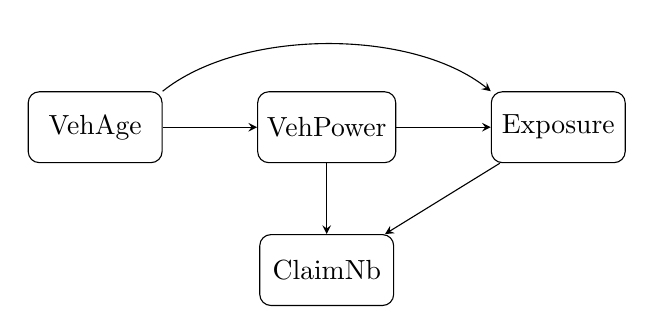
\begin{tikzpicture}[
    every node/.style={draw, rectangle, rounded corners, minimum width=1.7cm, minimum height=0.9cm, align=center},
    >=stealth,
    node distance=1.2cm % reduced vertical gap
]

% Nodes
\node (VehAge) {VehAge};
\node[right=of VehAge] (VehPower) {VehPower};
\node[right=of VehPower] (Exposure) {Exposure};
\node[below=0.9cm of VehPower] (ClaimNb) {ClaimNb};

% Edges
\draw[->] (VehAge) -- (VehPower);
\draw[->] (VehAge.north east) .. controls +(1.0,0.8) and +(-1.0,0.8) .. (Exposure.north west);
\draw[->] (VehPower) -- (Exposure);
\draw[->] (VehPower) -- (ClaimNb);
\draw[->] (Exposure) -- (ClaimNb);

\end{tikzpicture}
\caption{Causal graph estimated by CPCM on the French motor insurance dataset subset.}
\label{Fig_motor}
\end{figure}







\iffalse
\subsection{Illustration using income and expenditure dataset}

We explain our methodology in detail based on real-world data that describes the expenditure habits of Philippines residents. The Philippine Statistics Authority conducts a nationwide survey of Family Income and Expenditure \citep{psa_fies} every three years. 
The dataset (taken from \cite{FamilyIncomeExpenditure}) contains over 40,000 observations primarily comprising the household income and expenditures of each household. To reduce the size and add homogeneity to the data, we consider only families of size $1$ (people living alone) above the poverty line (top 90\%, with an income of at least $80,000\,\, pesos\approx 4000\,\,dollars $ per year). We end up with $n=1417$ observations. We focus on the following variables: Total income ($X_1$), Food expenditure ($X_2$), and Alcohol expenditure ($X_3$). 

These data exhibit strong heavy-tailed behavior, presenting a significant challenge for most causal discovery approaches. For instance, while $95\%$ of the population has an annual income below $400,000\,\text{pesos}$, the top $1\%$ far exceeds $1,000,000\,\text{pesos}$. This tail structure suggests the possibility of infinite variance and even an infinite expected value for all variables. Consequently, ANM and location-scale models are highly unsuitable in this context, since $f(x) = \mathbb{E}[X_i\mid X_j=x]=\infty$. In contrast, our $CPCM(F)$ method is well-suited for heavy-tailed settings when employing a heavy-tailed choice of $F$. In economics, it is common practice to model income using Pareto or Gamma distributions \citep{lawless2002statistical}.


Our objective is to identify the causal relationships among these variables. Common sense suggests that \( \text{Income} \to \text{Food} \). However, the relationships between alcohol and other variables are not trivial. In order to discovery causal relations, we apply our \( CPCM(F_1, \dots, F_k) \) methodology, following the algorithm presented in Section \ref{Section_Algorithm}. Choice \( \{F_1, \dots, F_k\} = \mathscr{S}_1 \) leads to strong rejection of all tests, making no direction plausible. This is not surprising, as the sample size is relatively large for a single parameter to sufficiently describe the complex behavior of the data. Hence, we choose \( \{F_1, \dots, F_k\} = \mathscr{S}_2 \), as defined in Section~\ref{Section_practical_choices}. 

First, we focus on the causal relationships between pairs of random variables.  Applying Algorithm~\ref{Algorithm1} to determine the causal relationship between \( X_1 \) and \( X_2 \) yields p-values of 0.2 and 0.02 for the directions \( X_1 \to X_2 \) and \( X_2 \to X_1 \), respectively. This suggests rejecting the plausibility of the latter graph while not rejecting the former, leading to the final estimation \( X_1 \to X_2 \). Using a similar approach, we conclude that \( X_3 \to X_2 \), with p-values of \( 2 \times 10^{-9} \) and 0.16. This result suggests that drinking habits influence food habits. Finally, the p-values corresponding to \( X_1 \to X_3 \) and \( X_3 \to X_1 \) were \( 10^{-9} \) and 0.02, respectively. This indicates that some assumptions remain unfulfilled. In this case, we believe that causal sufficiency is violated due to a strong unobserved common cause between these variables. Note that even though both causal graphs were implausible, the direction \( X_3 \to X_1 \) appeared to be more probable (\(0.02 > 10^{-9} \)).

Finally, we apply the multivariate score-based algorithm presented in Section \ref{Section_score_based_algorithm} using the choice \( \{F_1, \dots, F_k\} = \mathscr{S}_2 \). The graph with the best score is \( \text{Alcohol} \to \text{Food} \leftarrow \text{Income} \). However, this graph is not plausible, as the test of independence between \( \hat{\varepsilon}_1, \hat{\varepsilon}_2, \hat{\varepsilon}_3 \) yields a p-value of 0.03. This suggests that some assumptions, such as causal sufficiency, may still be violated. 

\fi
\section{Conclusion and future research}


We introduced a new family of models for causal inference called Conditionally Parametric Causal Models (CPCM), designed to flexibly accommodate a broad range of variable types and distributional forms. Our primary theoretical contributions lie in establishing the identifiability conditions for the causal structure within this framework. Specifically, we have demonstrated that the bivariate $CPCM(F)$ models are identifiable, with exceptions arising only when the parameters of $F$ take the form of a linear combination of its sufficient statistics. Furthermore, we have provided detailed characterizations of identifiability across various cases such as Gaussian, Poisson, and Pareto, significantly broadening the scope of identifiable models beyond existing literature. We also explained the multivariate extensions of these results. 

We complement these results with two consistent estimation algorithms for CPCM-based causal graph recovery. Experiments show competitive performance in Gaussian location–scale models, while retaining the ability to operate in much broader distributional settings, including heavy-tailed, continuous, discrete or even a mixture of these. 

CPCM also connects naturally to invariant causal prediction (\cite{Peters_invariance, Kook03042025}), offering promising directions for distribution-aware causal feature selection, as the framework of target-variable causal modelling provides a natural environment for embedding the CPCM ideology \citep{Bodik_biometrika}. Extensions to uncertainty quantification under distribution shift \citep{liu2021learning} or time series settings \citep{Bodik}  would further broaden its applicability. Integrating these ideas and validating CPCM in diverse applied domains are key avenues for future work.





\section*{Conflict of interest and data availability}
The open-source implementation of the methods discussed in this manuscript together with the data used can be found in the supplementary package or at \url{https://github.com/jurobodik/Causal_CPCM.git}.

The authors declare that they have no known competing financial interests or personal relationships that could have appeared to influence the work reported in this paper.


\section*{Acknowledgments}
This study was supported by the Swiss National Science Foundation under grant number 201126. 


































































\newpage
%\appendix


\pagenumbering{arabic}% Arabic page numbers (and reset to 1)
\renewcommand*{\thepage}{A\arabic{page}}



\begin{center}
\Large \textbf{Appendix}
\end{center}
This appendix is organized as follows:
\begin{itemize}
    \item Appendix~\ref{Appendix_A} provides a detailed definition and assumptions concerning the Exponential family, which were omitted from the main text for clarity. It also introduces the notion of F-suitability of an estimator and includes an in-depth discussion and proof of Proposition~\ref{consistency_proposition}.
    \item Appendix~\ref{Appendix_simulations} presents additional experiments and elaborates on certain implementation details.
    \item Appendix~\ref{SectionProofs} contains all theoretical results along with their corresponding proofs.
\end{itemize}


\renewcommand\thesection{A}
\section{Exponential family and Proposition \ref{consistency_proposition}}
\label{Appendix_A}

\subsection{Exponential family}
\label{appendix_exponential_family}

The exponential family is a set of probability distributions whose probability density function can be expressed in the following form:
\begin{equation}\tag{\ref{Exponential family of distributions}}
f(x;\theta) = h_1(x)h_2(\theta)\exp\big[\sum_{i=1}^q\theta_iT_i(x)\big],
\end{equation}
where $h_1, T_i$ are real functions and $h_2:\mathbb{R}^q\to\mathbb{R}^+$ is a vector-valued function. We call $T_i$ a \textit{sufficient} statistic, $h_1$ a base measure, and $h_2$ a normalizing (or partition) function.  

Often, form (\ref{Exponential family of distributions}) is called a canonical form and $$f(x;\theta) = h_1(x)h_2(\theta)\exp\big[\sum_{i=1}^qh_{3,i}(\theta)T_i(x)\big],$$ where  $h_{3,i}:\mathbb{R}^q\to\mathbb{R}, i=1, \dots, q$, is called its \textit{reparametrization} (natural parameters are a specific form of the reparametrization). We always work only with a canonical form (attention for Gaussian distribution, where the standard form is not in the canonical form). 

Numerous important distributions lie in the exponential family of distributions, such as Gaussian, log-normal, Poisson, Pareto (with fixed support), Weibull, chi-squared, multinomial, Binomial, Gamma, and Beta distributions, to name a few. 

It is important to note that functions in (\ref{Exponential family of distributions}) are \textit{not} uniquely defined. For example, $T_i$ is unique up to a linear transformation. 

The support of $f$ is fixed and does not depend on $\theta$. Potentially, $T_i$ and $h_1$ do not have to be defined outside of this support; however, we typically overlook this fact (or possibly define $h_1(x) = T_i(x) = 0$ for $x$ where these functions are not defined). We additionally assume that the support is nontrivial in the sense that it contains at least two distinct values.





Without loss of generality, we assume that $q$ is minimal in the sense that $f(x; \theta)$ cannot be expressed using only $q - 1$ parameters. The sufficient statistics $T_1, \dots, T_q$ are then linearly independent in the following sense: there exist points $x_1, \dots, x_q \in \operatorname{supp}(f)$ such that the matrix 
\begin{equation}\label{eq2431087}
\begin{pmatrix}
T_{1}(x_1) & \cdots & T_{{q}}(x_1) \\
\cdots & \ddots & \cdots \\
T_{1}(x_q) & \cdots & T_{{q}}(x_{q}) 
\end{pmatrix} 
\end{equation}
has full rank. Moreover, $T_1, \dots, T_q$ are affinly independent in the following sense: there exist $y_0, y_1, \dots, y_q\in supp(f)$, such that a matrix 
\begin{equation}\label{eq145151}
\begin{pmatrix}
T_{1}(y_1) - T_1(y_0) & \cdots & T_{{q}}(y_1) -T_q(y_0)\\
\cdots & \ddots & \cdots \\
T_{1}(y_q) -T_1(y_0) & \cdots & T_{{q}}(y_{q}) -T_q(y_0)
\end{pmatrix} 
\end{equation}
has full rank. In this paper—specifically in Lemma~\ref{PomocnaLemma1}—we assume affine independence of $T_1, \dots, T_q$, i.e., that condition~\eqref{eq145151} holds.

Since the notions of linear and affine independence used here are nonstandard, we illustrate them with a simple example. Let $T_1(x) = x$ and $T_2(x) = x^2$, corresponding to the sufficient statistics of a Gaussian distribution. Then matrices \eqref{eq2431087} and \eqref{eq145151} become: 
\begin{equation*}
M_1=\begin{pmatrix}
x_1 &  x_1^2\\
x_2  & x_{2}^2
\end{pmatrix} , \,\,\,\,
M_2=\begin{pmatrix}
y_1-y_0 &  y_1^2 -y_0^2\\
y_2 -y_0 &  y_2^2 -y_0^2
\end{pmatrix} ,
\end{equation*}
both of which are full-rank for the choices $(x_1, x_2) = (1,2)$ and $(y_0, y_1, y_2) = (0,1,2)$, for instance. 

\subsection{F-suitability and Proposition~\ref{consistency_proposition} }
\label{Appendix_consistency}



\subsubsection{Suitability of an estimator}
In the following, we define an $F$-suitable estimator for a given distribution function $F$ with parameters $\theta$. This is a modification of the concept of a suitable estimator for the conditional expectation discussed in \cite[Appendix A.2]{reviewANMMooij}. In case when $F$ is location-distribution (such as Gaussian distribution with fixed variance), our results fully align with \citep{reviewANMMooij}. 


Let $(X_{i}, Y_{i})_{i=1}^n$ be a random sample from $(X, Y)$. We say that the estimator $\hat{\theta}$ is \textbf{F-suitable for $X \to Y$} if the following conditions are satisfied:

\begin{itemize}
    \item \textbf{(Existence of a point-wise limit)} There exists $\theta$ such that $\hat{\theta}(x) \overset{P}{\to} \theta(x)$ as $n\to\infty$ for all $x\in supp(X)$. Moreover, if it is possible to write  $Y = F^{-1}(\varepsilon_2; \tilde{\theta}(X))$, with $X\indep \varepsilon_2\sim Unif(0,1)$, then this limit is equal to $\theta= \tilde{\theta}$. 
    \item \textbf{(Weak residual consistency)} It holds that
\begin{equation}
    \label{gdert}
    \lim_{n\to\infty}\mathbb{E}_{}\left( \frac{1}{n}\sum_{i=1}^n(\varepsilon_i-\hat{\varepsilon}_i)^2 \right) = 0,
\end{equation}
where $\varepsilon_i := F(Y_{i}; \theta(X_{i}))$ and $\hat{\varepsilon}_i := F(Y_{i}; \hat{\theta}(X_{i})), i=1, \dots, n$ and where the expectation is taken with respect to the distribution of the random sample.
\end{itemize}

We say that the estimator $\hat{\theta}$ is \textbf{F-suitable} if it is F-suitable for both $X \to Y$ and $Y \to X$. We simply write that  $\hat{\theta}$ is ``suitable'' if $F$ is evident from the context. 

\subsubsection{Literature review - which estimators are suitable?}

\textbf{Location family:} when $F$ is location-family distribution, such as a Gaussian distribution with fixed variance, property \eqref{gdert} reduces to classical notion of a weak universal consistency:
\(
\lim_{n\to\infty}\mathbb{E}[||\theta(X) - \hat{\theta}(X)||^2] = 0.
\) Such consistency have been already discussed also in relation to causal discovery \citep{zhang2015estimation,uemura2022multivariate, keropyan2023rank}. 
The weak universal consistency has been established for various estimators under appropriate smoothness assumptions on $\theta$. Examples of such estimators include:
\begin{itemize}
    \item Kernel estimators (see Theorem 5.1 in \cite{Gyorfi2002})
    \item Smoothing spline GAM estimators (see Chapter 14.2 in \cite{Gyorfi2002}, \cite{claeskens2009} or \cite{Wood2})
    \item Neural networks (see Theorem 16.1 in \cite{Gyorfi2002} or \cite{drews2022universalconsistencyoverparametrizeddeep}).
\end{itemize}
Importantly, these consistency results apply regardless of the causal direction. In the anti-causal direction, we have \( X = \theta(Y) + \varepsilon \), where \( \theta(Y) = \mathbb{E}[X \mid Y] \) and \( \varepsilon \not\indep Y \), \( \mathbb{E}[\varepsilon \mid Y] = 0 \). Note that  \( \varepsilon \not\indep Y \) holds if and only if the model is identifiable. For such case, the same form of weak consistency remains valid for the estimators listed above (again, under appropriate smoothness assumptions).

\textbf{Location-scale family:} when $F$ is a location-scale distribution (e.g. Gaussian), several consistency results has also been established for various estimators under appropriate smoothness and regularity assumptions, see e.g. \cite{10.1093/biomet/85.3.645}, or \cite{immer2022identifiability, Siegfried02102023, Le_Smola}. 

\textbf{More general families:} Consistency results for non-Gaussian families are less explored in nonparametric settings, with most existing literature focusing on empirical evidence. GAMLSS \citep{GAMLSS} offers a broad class of estimators, with \cite{GAMLSS_webpage} presenting extensive empirical evidence on simulations and hundreds of real-data examples demonstrating consistency. A few theoretical results are avaliable for GAM estimators; e.g. Theorem 1 in \cite{GAMSamworthConsistency} establishes its almost sure universal consistency for a general one-dimensional exponential family of distributions for \( Y \mid X \), assuming certain smoothness and convexity/monotonicity conditions on \( \theta \). \cite{Wood2} discusses general framework for smoothing parameter estimation for models with regular likelihoods constructed in terms of unknown smooth functions of covariates.   \cite{mammen1997} discusses the consistency under partial linearity assumption.  


\subsubsection{HSIC score}

For the definition and discussion of the HSIC score, see \cite[Appendix A.1]{reviewANMMooij}. We use the same notation and implicitly use bounded non-negative Lipschitz-continuous kernels such that their product is characteristic, as in the "Data recycling" scenario in \cite[Corollary 21]{reviewANMMooij}.

\subsubsection{Proof of Proposition~{\ref{consistency_proposition}}}

\begin{customprop}{\ref{consistency_proposition}}
Let $(X_1, X_2)$ follow an identifiable $CPCM(F_1, \dots, F_k)$ with DAG $\mathcal{G}$. Then, our score-based algorithm presented in Section~\ref{Section_score_based_algorithm} is consistent, meaning that
$$\hat{\mathcal{G}} \overset{P}{\to}\mathcal{G}\,\,\,as\,\,n\to\infty,$$
given that we employ a “suitable” estimation procedure for the estimator  $\hat{\varepsilon}_i$, we use HSIC score as our choice of $\rho$ and consistent estimates of $S_i$. 
\end{customprop}


\begin{proof}
The proof mostly aligns with the proof of Corollary 21 in \cite{reviewANMMooij}. We use the notation $X = X_1$ and $Y = X_2$.

If $X \indep Y$, then $\hat{\mathcal{G}}$ converges to an empty graph, since any other graph has a score of at least $\lambda$ and $\hat{\varepsilon}_1, \dots, \hat{\varepsilon}_d$ are independent by definition. From now on, without loss of generality, let $Y = F_j^{-1}(\varepsilon_2; \theta(X)), \varepsilon_2\indep X$ for some  $j \in \{1, \dots, k\}$. Denote by $\mathbf{x} = (x_1, \dots, x_n)$ and $\mathbf{y} = (y_1, \dots, y_n)$ the observed data. In the following, we compare the asymptotic scores of graphs $X\to Y$ and $Y\to X$. 

\textbf{Graph} $X \to Y$: Define the ``population residual'' \(E_Y := F_j(Y; \theta(X))\) and the ``estimated residual'' $\hat{\varepsilon}_Y^i = (F_i(y_l; \hat{\theta}(x_l)))_{l=1}^n$, where $i=1, \dots, k$. For the true $i = j$, we omit the superscript and write $\hat{\varepsilon}_Y = (F_j(y_l; \hat{\theta}(x_l)))_{l=1}^n$. By construction, \(X \perp\!\!\!\perp E_Y\) which implies \(\text{HSIC}(X, E_Y) = 0\) (due to Lemma 12 in \cite{reviewANMMooij}). 

Now, since the estimator $\hat{\theta}$ satisfies \eqref{gdert}, we can use the argument presented in \cite[Theorem 20]{reviewANMMooij}, and obtain $\widehat{HSIC}(\mathbf{x}, \hat{\varepsilon}_y) \xrightarrow{P} \text{HSIC}(X, E_Y)$. 

Since $\hat{S}_2$ is consistent, we can find $n_0$ such that for all $n\geq n_0$ holds $P(j\in\hat{S}_2)\geq 1-\delta$ for given $\delta>0$. 

Putting everything together, with probability larger than $1-\delta$ holds

\begin{equation*}
    \begin{split}
        s(X \to Y) &= \min_{j_2 \in \hat{S}_2}\rho(\mathbf{x}, \hat{\varepsilon}_y^{j_2}) + \lambda \leq \rho(\mathbf{x}, \hat{\varepsilon}_y) + \lambda \\
        &= \widehat{HSIC}(\mathbf{x}, \hat{\varepsilon}_y) + \lambda \xrightarrow{P} \text{HSIC}(X, E_Y) + \lambda = \lambda.
    \end{split}
\end{equation*}
By sending $\delta\to 0$, we obtain $  s(X \to Y)\xrightarrow{P} \lambda $. 

\textbf{Graph} $Y \to X$: Define the ``population residual'' \(E_X^j := F_j(X; \theta_j(Y))\) and the ``estimated residual'' $\hat{\varepsilon}_X^j = (F_j(x_i; \hat{\theta}_j(y_i)))_{i=1}^n$, where $\theta_j$ is the limit of $\hat{\theta}_j$ defined in the definition of $F_j$-suitability. 

Due to the assumption of identifiability, $Y\not\indep E_X^j$ for all $j\in\{1, \dots, k\}$. Therefore, using Lemma 12 in \cite{reviewANMMooij}, we have \(\text{HSIC}(Y, E_X^j) > 0\). Again, since the estimator $\hat{\theta}$ satisfies \eqref{gdert}, we can use the argument presented in \cite[Theorem 20]{reviewANMMooij}, and obtain $\widehat{HSIC}(\mathbf{y}, \hat{\varepsilon}_X^j) \xrightarrow{P} \text{HSIC}(Y, E_X^j)$. 


Putting everything together
\begin{equation*}
    \begin{split}
        s(Y \to X) &= \min_{j \in \hat{S}_1}\rho(\mathbf{y}, \hat{\varepsilon}_x^j) + \lambda \geq \min_{j \in \{1, \dots, k\}}\widehat{HSIC}(\mathbf{y}, \hat{\varepsilon}_X^j) + \lambda \\
        &  \xrightarrow{P} \min_{j \in \{1, \dots, k\}}\text{HSIC}(Y, E_X^j) + \lambda > \lambda, \,\,\,\,\,\,\,\,\,\,\,\text{as}\,\,n\to\infty.
    \end{split}
\end{equation*}
Therefore, the score for the correct direction is asymptotically smaller than that for the wrong causal direction as $n \to \infty$, hence the procedure is consistent.
\end{proof}


\begin{customconsequence}{\ref{consequence_consistency}}
Let $(X_1, X_2)$ follow an $CPCM(F)$ model with DAG $\mathcal{G}$, for some $F\in\mathscr{S}_1\cup \mathscr{S}_2$. Assume the conditions of Proposition~\ref{consistency_proposition} hold: namely, identifiability of $CPCM(\mathscr{S}_1 \cup \mathscr{S}_2)$, a suitable estimation procedure, and the use of the HSIC score. Then, our score-based algorithm, with the collection $\{F_1, \dots, F_k\}$ chosen via the Sequential approach (Exact or Fast
version), is consistent:
$\hat{\mathcal{G}} \overset{P}{\to}\mathcal{G}$, as $n\to\infty$.
\end{customconsequence}


\begin{proof}

If $F \in \mathscr{S}_1$, the result follows directly from Proposition~\ref{consistency_proposition}. Similarly, if $F \in \mathscr{S}_2$ and the Sequential approach returns $\mathscr{S}_1 \cup \mathscr{S}_2$, the proposition again directly applies.

It remains to consider the case where $F \in \mathscr{S}_2$ but the Sequential approach returns only $\mathscr{S}_1$. We will show that, as $n \to \infty$, this event occurs with probability tending to zero. In other words, when $F \in \mathscr{S}_2$, the Sequential approach will return $\mathscr{S}_1 \cup \mathscr{S}_2$ with probability tending to one.


If $X \indep Y$, then $\hat{\mathcal{G}}$ converges to an empty graph regardless of the choices of $F$. Hence, without loss of generality, assume non-empty causal graph. Consider graph $\mathcal{G} = X_1 \to X_2$, and take some $F_1 \in \mathscr{S}_1$ (that is, wrong distribution $F_1\neq F$). In this case, following the notation of the proof of Proposition~\ref{consistency_proposition}, we have
\begin{equation}
\label{eq2345}
    \widehat{\text{HSIC}}(\mathbf{x}_1, \hat{\varepsilon}_{X_2}^{1}) \xrightarrow{P} \text{HSIC}(X_1, E_{X_2}^{1}) > 0,
\end{equation}
where $\hat{\varepsilon}_{X_2}^{j} := (F_j\big(X_2; \hat{\theta}_j(X_1)\big))_{l=1}^n$ is the vector of residuals obtained by applying a ``suitable'' estimation procedure, and the ``population residual'' \(E_{X_2}^{j} := F_j(X_2; \theta(X_1))\). This convergence follows from the same reasoning as in the `$Y \to X$' case in the proof of Proposition~\ref{consistency_proposition}. 

In particular, \eqref{eq2345} implies that the variance of the empirical HSIC statistic vanishes:
\[
\operatorname{Var} \left( \widehat{\text{HSIC}}(\mathbf{x}_1, \hat{\varepsilon}_{X_2}^{1}) \right) \to 0 \quad \text{as } n \to \infty.
\]
Therefore, according to the construction of confidence intervals for the HSIC test in~\cite[Section~3.2.2]{Kernel_based_tests}, the $(1 - \alpha)$ confidence interval will eventually lie entirely within an interval of the form $[\mathrm{HSIC}(X_1, E_{X_2}^{1}) - \delta, \mathrm{HSIC}(X_1, E_{X_2}^{1}) + \delta]$, for arbitrarily small $\delta > 0$. Since the limiting HSIC value is strictly positive, this interval will exclude $0$ for large enough $n$, yielding p-values smaller than $\alpha$. As a result, the DAG $\mathcal{G}$ will be rejected as plausible.

The same argument applies to the case $\mathcal{G} = X_2 \to X_1$ and for any $F_j \in \mathscr{S}_1$, $j = 1, \dots, k$. Therefore, for sufficiently large $n$, no DAG will be deemed plausible, and the Sequential approach will return the full set $\mathscr{S}_1 \cup \mathscr{S}_2$ with high probability.
\end{proof}


\begin{lemma}[Consistency of Algorithm 1 under unidentifiability]
Let $(X_1, X_2)$ follow an \textit{\textbf{unidentifiable}} model $CPCM(F_1, \dots, F_k)$ with DAG $\mathcal{G}$. Suppose the HSIC independence test is used in step 1b) of Algorithm 1, and assume access to an oracle regression estimator $\hat\theta = \theta$. Then, for sufficiently large $n$, Algorithm 1 outputs “Unidentifiable case” with probability at least $1 - 2\alpha$.
\end{lemma}

\begin{proof}
If the true model is unidentifiable, independence holds in both directions: $X_1 \indep \varepsilon_2$ and $X_2 \indep \varepsilon_1$. Given an oracle regression estimator $\hat\theta = \theta$, we have $\hat\varepsilon_i = \varepsilon_i$ for $i = 1, 2$. Therefore, Algorithm 1 reduces to performing two HSIC independence tests and returning “Unidentifiable case” if both tests fail to reject the null.

The HSIC test has asymptotically correct level under the null hypothesis of independence (\cite{Kernel_based_tests}, Theorem 3.8). Thus, for sufficiently large sample size $n$, the probability that the HSIC test fails to reject the null in each direction is at least $1 - \alpha$. By the union bound, the probability that both tests fail to reject is at least $(1 - \alpha)^2 > 1 - 2\alpha$. Hence, Algorithm 1 returns “Unidentifiable case” with probability at least $1 - 2\alpha$.
\end{proof}

\renewcommand\thesection{B}
\section{Experiments details and additional plots}
\label{Appendix_simulations}

\subsection{Exact, Naive-greedy, RESIT, and RESIT-greedy algorithms: definitions and comparison}
\label{appendix_greedy_definitions}
We consider the following algorithms for estimating the underlying causal graph from observational data using the CPCM score function~\eqref{score_definition1}:

\begin{itemize}
    \item \textbf{Exact search:} This algorithm evaluates the CPCM score for all DAGs on $d$ nodes and selects the one with the lowest score. Since the number of DAGs grows super-exponentially with $d$ (e.g., 29,281 DAGs for $d = 5$), exact search is computationally feasible only for very small graphs with $d \leq 4$.
    
    \item \textbf{Naive-edge-greedy:} Starting from an empty DAG, this algorithm iteratively explores neighboring DAGs by adding or removing a single edge. At each step, it selects the neighboring graph with the lowest CPCM score and replaces the current graph if the score improves. The procedure stops when no further improvement is possible. While simple and scalable, this greedy approach lacks theoretical guarantees and may get stuck in local minima, unless we assume some advanced notions of convexity over the space of all DAGs.

    \item \textbf{RESIT (Regression with Subsequent Independence Test):} RESIT first estimates a topological ordering by iteratively selecting the variable whose residual is least dependent on the remaining variables. In the second phase, it removes superfluous edges using conditional independence tests. See Algorithm~\ref{alg:resit} for details. The procedure is computationally efficient and comes with statistical guarantees (see Lemma~\ref{thm:resit_consistency}). However, empirical performance tends to be worse than that of greedy algorithms, particularly due to the accumulation of errors in the ordering phase and false positives (type I errors) in the Phase~2. 

    \item \textbf{RESIT-greedy:} This hybrid algorithm combines the topological ordering phase of RESIT with the edge-pruning phase of naive-greedy search. After estimating the ordering, it starts with a fully connected DAG consistent with the order and iteratively removes edges that lead to the largest improvement in the CPCM score, until no further improvement is possible. See Algorithm~\ref{alg:resit_greedy}.
\end{itemize}
\citet{Peters2014} showed that, in the population case, the RESIT algorithm is consistent under identifiable additive noise models, assuming a consistent nonparametric regression method and a perfect independence oracle. The same reasoning applies directly to CPCM models.


\begin{lemma}[Consistency of RESIT under CPCM]
\label{thm:resit_consistency}
Let $\mathbf{X}$ be generated by a $CPCM(F_1, \dots, F_k)$ model with underlying DAG $\mathcal{G}_0$. Then, the RESIT algorithm, when applied with consistent estimators $\hat{\theta}_k$ and an independence oracle, is guaranteed to recover the true graph $\mathcal{G}_0$ from the distribution of $\mathbf{X}$.
\end{lemma}

\begin{proof}
A direct consequence of Theorem~34 in \citet{Peters2014}. Note that we implicitly assume the causal minimality condition for $CPCM(F_1, \dots, F_k)$ as stated in Definition~\ref{DefinitionCPCM}.
\end{proof}

\begin{algorithm}[]
\caption{Regression with Subsequent Independence Test (RESIT)}
\label{alg:resit}
\KwIn{I.i.d. samples of a $d$-dimensional distribution on $(X_1, \ldots, X_d)$}
$S \gets \{1, \ldots, d\}; \pi \gets [\ ]$\;

\textbf{Phase 1: Determine topological order $\pi$} \;
\While{$S \ne \emptyset$}{
  \ForEach{$k \in S$}{
    Compute residuals $\hat{\varepsilon}_k := F\big(X_k; \hat{\theta}_k(\mathbf{X}_{S \setminus \{k\}})\big)$\;
    Measure dependence between $\hat{\varepsilon}_k$ and $\{X_i\}_{i \in S \setminus \{k\}}$\;
  }
  Let $k^* \gets$ variable with weakest dependence\;
  $S \gets S \setminus \{k^*\}$\;
  $\mathrm{pa}(k^*) \gets S$\;
  Prepend $k^*$ to $\pi$\;
}

\textbf{Phase 2: Remove superfluous edges} \;
\For{$k = 2$ \KwTo $d$}{
  \ForEach{$\ell \in \mathrm{pa}(\pi_k)$}{
    Compute residuals:
    $\hat{\varepsilon}_{\pi_k} := F\big(X_{\pi_k}; \hat{\theta}_{\pi_k}(\mathbf{X}_{\mathrm{pa}(\pi_k) \setminus \{\ell\}})\big)$\;
    \If{$\hat{\varepsilon}_{\pi_k}$ is independent of $\{X_{\pi_1}, \ldots, X_{\pi_{k-1}}\}$}{
      $\mathrm{pa}(\pi_k) \gets \mathrm{pa}(\pi_k) \setminus \{\ell\}$\;
    }
  }
}
\KwOut{$(\mathrm{pa}(1), \ldots, \mathrm{pa}(d))$}
\end{algorithm}





\begin{algorithm}[]
\caption{RESIT-greedy}
\label{alg:resit_greedy}
\KwIn{I.i.d. samples of a $d$-dimensional distribution on $(X_1, \ldots, X_d)$}

\textbf{Phase 1: Determine topological order $\pi$} \;
As in RESIT (Algorithm~\ref{alg:resit})\;

\textbf{Phase 2: Greedy removal of edges using CPCM score} \;
Initialize graph $\mathcal{G}$ with all edges $(j \to i)$ such that $j \in \mathrm{pa}(i)$ and $j$ precedes $i$ in $\pi$\;

\Repeat{\textbf{no score improvement}}{
  $\mathcal{G}_{\text{best}} \gets \mathcal{G}$\;
  $S_{\text{best}} \gets \text{CPCM}(\mathcal{G})$\;

  \ForEach{edge $e = (j \to i)$ in $\mathcal{G}$}{
    $\mathcal{G}' \gets \mathcal{G}$ with $e$ removed\;
    $S' \gets \text{Score of }\mathcal{G} \text{ in }\text{CPCM}$ \eqref{score_definition1}\;

    \If{$S' < S_{\text{best}}$}{
      $\mathcal{G}_{\text{best}} \gets \mathcal{G}'$\;
      $S_{\text{best}} \gets S'$\;
    }
  }

  \If{$\mathcal{G}_{\text{best}} \ne \mathcal{G}$}{
    $\mathcal{G} \gets \mathcal{G}_{\text{best}}$\;
  } \Else{
    \textbf{break}\;
  }
}
\KwOut{$\mathcal{G}$}
\end{algorithm}



\subsubsection{Experiments: comparison of different greedy algorithms}
\label{appendix_greedy}
\textbf{Data-generating process:} We generate  random DAGs uniformly over $d$ nodes with $p$ edges, where $p \sim \mathrm{Exp}(1/d)$ and capped at $\frac{d(d-1)}{2}$. On average, each DAG contains approximately $d$ edges. For a given DAG $\mathcal{G}$, we simulate data from the $CPCM(F)$ model, $F=Exponential$, defined as:
$$
X_i \sim \mathrm{Exp}\left(\lambda(\mathbf{X}_{pa_i(\mathcal{G})})\right), \quad \text{with} \quad \lambda(\mathbf{X}_{pa_i(\mathcal{G})}) = \frac{1}{\sum_{j \in pa_i(\mathcal{G})} |X_j|} = \frac{1}{\mathbb{E}[X_i\mid \textbf{X}_{pa_i}]}.
$$
If $pa_i(\mathcal{G})=\emptyset$, then $X_i\sim N(0,1)$. Using $n = 1000$ samples, we estimate $\mathcal{G}$ using the score-based CPCM estimator defined in Equation~\eqref{score_definition1}, with a fixed function class $\mathscr{S}_1$ (rather than the sequential approach) to allow for a fair comparison in both accuracy and computational cost. We compare the Exact, Naive-greedy, RESIT, and RESIT-greedy methods.  We evaluate their performance using the Structural Intervention Distance (SID, \cite{peters2014structuralinterventiondistancesid}), computing $\mathrm{SID}(\mathcal{G}, \hat{\mathcal{G}})$ for each estimated graph.

\textbf{Results:} Figure~\ref{figure_greedy} presents the average normalized $\frac{SID}{d}$ over 50 repetitions.

\begin{itemize}
    \item The exact method achieves, unsurprisingly, the lowest SID, with the highest computational cost. 
    \item Both RESIT and naive-greedy exhibit similar performance. The greedy approach achieves slightly lower SID on average but requires slightly more computation time. Note that for $d\geq 8$, both methods perform as badly as Trivial algorithm (empty graph).
    \item RESIT-greedy serves as a middle ground: it significantly improves over RESIT/naive-greedy methods in terms of SID while incurring higher computational cost for $d > 5$.
\end{itemize}


These experiments highlight the trade-offs between statistical performance and computational efficiency among the evaluated methods. While the exact method yields the most accurate graph recovery, its scalability is limited. In contrast, RESIT and naive-greedy offer faster but less accurate alternatives, with performance deteriorating as graph complexity increases. RESIT-greedy provides a promising compromise, achieving lower SID than standard greedy methods at a moderate computational cost. \textbf{Overall, RESIT-greedy seems to be a practical choice in graphs with size} $4<d<10$.

\begin{figure}[]
\centering
\includegraphics[scale=0.62]{figures/greedy_comp.pdf}
\caption{Performance of different greedy algorithms from Section~\ref{appendix_greedy}. Here, the trivial algorithm returns an empty graph. Runtime was measured on a machine with an Intel Core i5-6300U 2.5 GHz processor and 16 GB of RAM.}
\label{figure_greedy}
\end{figure}

\subsubsection{Statistical scalability: sample size needs to grow with increasing dimension}
\label{appendix_scalability}
Conducting independence tests and performing nonparametric regression becomes increasingly challenging as the number of covariates grows, particularly in high-dimensional settings, where such tasks demand substantially larger sample sizes. Similar limitations affect several existing algorithms, including ANM-RESIT, LOCI, and bQCD. As demonstrated below, the sample size required for consistent estimation increases systematically with the dimension~$d$.

\textbf{Data-generating process: }For each sample size \( n \) and dimension \( d \), we generated a uniformly random graph with \( d \) nodes and \( d-1 \) edges. The data was then generated according to the structural equation model \( X_i = f_i(\textbf{X}_{pa_i}) + \varepsilon_i \), where \( \varepsilon_i \sim N(0,1) \) and \( f_i(x) = c_i x^{2} \) with \( c_i \sim \text{Unif}(0.5, 1.5) \). 

\textbf{Results:}
We estimate the DAG using the $CPCM(F)$ algorithm, where $F$ is set to a Gaussian distribution with fixed variance, and apply the naive-greedy algorithm for structure learning. The accuracy of the estimated DAG is assessed using the Structural Intervention Distance (SID). This procedure is repeated 100 times, and we report the average SID. Figure~\ref{scalability} displays the ratio of the average SID from the CPCM(F) algorithm to the average SID of a baseline method that generates a random DAG.




\begin{figure}[]
\centering
\includegraphics[scale=0.6]{figures/scalability.pdf}
\caption{Ratio of the computed SID using the $CPCM(F)$ algorithm (edge-greedy version) to the SID of an algorithm producing a random graph, averaged over 100 repetitions for different values of \( n \) and \( d \). Lower SID fraction means better performance of the $CPCM(F)$ algorithm. Values around $SID\,fraction=1$ mean that our algorithm is no better than an algorithm producing a random graph.}
\label{scalability}
\end{figure}



\subsection{Sequential approach vs oracle: empirical performance}
\label{Simulations_seq_approach}
We evaluate the empirical performance of the sequential approach for selecting the distribution family, comparing it to $CPCM(F)$ with access to the true (oracle) distribution $F$. The data is generated as follows:
$$
X_1 \sim \mathcal{N}(0,1), \quad X_2 = F^{-1}(\varepsilon, \theta(X)), \quad \varepsilon \indep X, \; \varepsilon \sim \mathcal{U}(0,1),
$$
where $F \in \mathscr{S}_s$ belongs to either the one-parameter family $\mathscr{S}_1$ or the two-parameter family~$\mathscr{S}_2$.

When $s = 1$, $F$ is, with equal probability ($1/4$), either a Gaussian distribution with fixed variance, a Poisson, Pareto, or Exponential distribution. The parameter is generated as a random function of $X$ via a randomly drawn polynomial. When $s = 2$, $F$ is, again with equal probability, a Gaussian, Negative Binomial, Generalized Pareto, or Gamma distribution, with both parameters generated as random functions of $X$ using random polynomials.

We estimate the graph $\mathcal{G} = {1 \to 2}$ using both $CPCM(\text{Seq.app})$ and $CPCM(F)$ with oracle knowledge of $F$, for various sample sizes $n$, repeating each experiment 100 times for both $s = 1$ and $s = 2$. Figure~\ref{Fig_seq} summarizes the results across sample sizes.

For $s = 1$, we observe that $CPCM(\text{Seq.app})$ typically performs equivalently to oracle $CPCM(F)$ for $n > 100$. For $s = 2$, the sequential approach tends to select the simpler class $\mathscr{S}_1$ instead of the true two-parameter family $\mathscr{S}_2$ at smaller sample sizes. Nevertheless, the performance gap between the sequential approach and the oracle method remains almost negligible.

These results indicate that the sequential approach is performing nearly as well as the oracle $CPCM(F)$, provided that $F \in \mathscr{S}_1 \cup \mathscr{S}_2$.

\begin{figure}[]
\centering
\includegraphics[scale=0.7]{figures/Sequ.appr.pdf}
\caption{Performance of the sequential approach. Left: percentage of simulations where $\hat{\mathcal{G}} = {1 \rightarrow 2}$. Right: percentage of simulations in which $CPCM(\text{Seq.app})$ and $CPCM(F)$ with oracle $F$ are equivalent. }
\label{Fig_seq}
\end{figure}








\subsection{Details about sections~\ref{Section_simulations_Pareto}, \ref{Section_simulations_Gaussian}, \ref{Section_simulations_multivariate} and \ref{Section7}}

\label{Appendix_Section_simulations_Pareto}
The additional plots corresponding to \textbf{Section~\ref{Section_simulations_Pareto}} are presented in Table~\ref{Pareto_simulations1} and Figures~\ref{Pareto_histograms} and Figure~\ref{sample_size_pareto}. Figure~\ref{Simulations2_plots} shows an example of datasets generated via different models from Section~\ref{Section_simulations_Gaussian}.

% Please add the following required packages to your document preamble:
% \usepackage{multirow}
% \usepackage{graphicx}
\begin{table}[]
\centering
\renewcommand{\arraystretch}{1.15}
\begin{tabular}{l|
                S[table-format=3.0]
                S[table-format=3.0]
                S[table-format=3.0]
                S[table-format=3.0]
                S[table-format=3.0]}
\toprule
\textbf{$\gamma$} &
{$X_1 \to X_2$} &
{$X_2 \to X_1$} &
{\makecell{Empty\\graph}} &
{\makecell{Both directions\\appear plausible}} &
{\makecell{Neither direction\\appears plausible}} \\
\midrule
\rowcolor{RowAlt}
$-2$ & 0  & 0  & \bfseries 96 & 2  & 2  \\
$-1$ & 3  & 2  & 0  & \bfseries 95 & 0  \\
\rowcolor{RowAlt}
\,\,$0$  & 7  & 1  & 0  & \bfseries 92 & 0  \\
\,\,$1$  & 7  & 5  & 0  & \bfseries 86 & 2  \\
\rowcolor{RowAlt}
\,\,$2$  & \bfseries 93 & 0  & 0  & 14 & 3  \\
\bottomrule
\end{tabular}
\caption{Simulation results for the CPCM model using the Pareto distribution function \(F\). The table displays the percentage of cases for each type of graph structure estimated by Conservative Algorithm~\ref{Algorithm1} with the model specified in \eqref{fwesef}, across various values of the hyperparameter \(\gamma \in \mathbb{R}\). The columns indicate the frequency of each graph structure being estimated, with the highest frequency in each row highlighted in bold.}
\label{Pareto_simulations1}
\end{table}


\begin{figure}[]
\centering
\includegraphics[width = 0.8\textwidth]{figures/pareto_histogram.pdf}
\caption{(Simulations~\ref{Section_simulations_Pareto}). Distributions of the p-values from the independence test in Step 1b) of Algorithm~\ref{Algorithm1}, for model \eqref{fwesef} with \(\gamma = 0\) and \(\gamma = 2\).}
\label{Pareto_histograms}
\end{figure}


\begin{figure}[]
\centering
\includegraphics[scale=0.7]{figures/score_based_estimate.pdf}
\caption{(Simulations~\ref{Section_simulations_Pareto}). The plot displays the percentage of correctly estimated causal directions across a range of sample sizes \( n \), using model \eqref{fwesef} with hyperparameters \(\gamma = 1\) and \(\gamma = 2\). As \( n \) increases, the algorithm demonstrates near-perfect performance, affirming the theoretical consistency of the proposed method. }
\label{sample_size_pareto}
\end{figure}




The experiments from \textbf{Simulations~\ref{Section_simulations_Gaussian}} were inspired by \cite{Natasa_Tagasovska} and implementations of other baseline methods are also taken from \cite{Natasa_Tagasovska} and \cite{immer2022identifiability}. 

For LOCI, we use the default format with neural network estimations and subsequent independence testing (also denoted as $NN-LOCI_H$) \citep{immer2022identifiability}.
For IGCI, we use the original implementation from \cite{IGCI} with slope-based estimation with Gaussian and uniform reference measures. For RESIT, we use the implementation from \cite{Peters2014} with GP regression and the HSIC independence test with a threshold value of $0.05$. For the slope algorithm, we use the implementation of \cite{Slope}, with the local regression included in the fitting process. For comparisons with other methods such as PNL, GPI-MML, ANM, Sloppy, GR-AN, EMD, GRCI, see Section 3.2 in \cite{Natasa_Tagasovska} and Section 5 in \cite{immer2022identifiability}. 

In \textbf{Section~\ref{Section_simulations_multivariate}}, the other baseline methods are implemented using the \texttt{pcalg} package \citep{pcalg_package}, employing its default independence test \texttt{gaussCItest} for PC algorithm and GES with the Gaussian observational BIC score, using the default penalty. For ANM-RESIT, for fairness, we use the same choices as in our CPCM method (that is, GAM estimator and HSIC). 

Finally, regarding \textbf{Section~\ref{Section7}},  Table~\ref{tab:edge_share} shows the relative frequencies with which each edge was recovered across repeated subsamples of the motor insurance dataset.


\begin{figure}[]
\centering
\includegraphics[scale=0.4]{figures/sim6.2_sample.png}
\caption{Simulations~\ref{Section_simulations_Gaussian}. An example of datasets generated via different models. }
\label{Simulations2_plots}
\end{figure}



\begin{table}[ht]
\centering
\begin{minipage}{0.45\linewidth}
\centering
\begin{tabular}{lc}
\hline
Edge & Share (\%) \\
\hline
VehAge $\to$ ClaimNb     & 60 \\
Exposure $\to$ ClaimNb   & 48 \\
VehPower $\to$ ClaimNb   & 42 \\
VehPower $\to$ Exposure  & 44 \\
\hline
\end{tabular}
\end{minipage}\hfill
\begin{minipage}{0.45\linewidth}
\centering
\begin{tabular}{lc}
\hline
Edge & Share (\%) \\
\hline
VehAge $\to$ Exposure    & 36 \\
Exposure $\to$ VehAge    & 64 \\
VehPower $\to$ VehAge    & 54 \\
VehAge $\to$ VehPower    & 30 \\
\hline
\end{tabular}
\end{minipage}
\caption{Relative frequency (in \%) with which each directed edge was recovered by CPCM across 50 random subsamples of the French MTPL motor insurance dataset (shown only those with more than $25\%$ share).}
\label{tab:edge_share}
\end{table}










\renewcommand\thesection{C}
\section{Proofs}
\label{SectionProofs}

\subsection{Proof of Theorem~\ref{normalidentifiability}}
\begin{customthm}{\ref{normalidentifiability}}
Let $(X_1,X_2)$ admit the $CPCM(F)$ model with graph $X_1\to X_2$, where $F$ is the Gaussian distribution function with parameters $\theta(X_1)=\big(\mu(X_1), \sigma(X_1)\big)^\top$. 
Let $p_{\varepsilon_1}$ be the density of $\varepsilon_1$ that is absolutely continuous with full support $\mathbb{R}$. Let $\mu(x), \sigma(x)$ be two times differentiable.  

Then, the causal graph is identifiable from the joint distribution if and only if  there do not exist $a,c ,d,e, \alpha, \beta\in\mathbb{R}$,  
$a\geq 0,c>0, \beta>0$, such that
\begin{equation}\tag{\ref{norm}}
\frac{1}{\sigma^2(x)}=ax^2 + c, \,\,\,\,\,\,\,\,\,\,\,\,\,\,\,\,\,\,\,\,\, \frac{\mu(x)}{\sigma^2(x)}=d+ex,
\end{equation}
for all $x\in\mathbb{R}$ and
\begin{equation}\tag{\ref{DensityDEF}}
p_{\varepsilon_1}(x) \propto \sigma(x)e^{-\frac{1}{2}\big[ \frac{(x-\alpha)^2}{\beta^2}  - \frac{\mu^2(x)}{\sigma^2(x)}\big]},
\end{equation}
where $\propto$ represents an equality up to a constant (here, $p_{\varepsilon_1} $  is a valid density function if and only if $\frac{1}{\beta^2}\neq  \frac{e^2}{c}\mathbbm{1}[a=0]$). 
Specifically, if $\sigma(x)$ is constant (case $a=0$), then the causal graph is identifiable unless $\mu(x)$ is linear and $p_{\varepsilon_1}$ is the Gaussian density.
\end{customthm}



\begin{proof}
\label{Proof of normalidentifiability}{}
We opt for proving this theorem from scratch, without using Theorem \ref{thmAssymetricMultivariatesufficient}. An interested reader can try to use Theorem \ref{thmAssymetricMultivariatesufficient} instead. For clarity regarding the indexes, we use the notation $X=X_1, Y=X_2$. 

First, we show that if the causal graph is not identifiable, then $\mu(x)$ and $\sigma(x)$ must satisfy (\ref{norm}). Let $p_{(X,Y)}$ be the density function of $(X,Y)$. Since the causal graph is not identifiable, there exist two CPCM models that generate $p_{(X,Y)}$: the CPCM model with  $X\to Y$  and the function  $\theta(x)=\big(\mu(x), \sigma^2(x)\big)^\top$ and the CPCM model with  $Y\to X$ and the function $\tilde{\theta}(y)=\big(\tilde{\mu}(y), \tilde{\sigma}^2(y)\big)^\top$. 

We decompose (corresponding to the direction $X\to Y$) 
\begin{equation*}
p_{(X,Y)}(x,y) = p_{X}(x)p_{Y\mid X}(y\mid x) = p_{X}(x) \phi\big(y;\theta(x)\big),
\end{equation*}
where $\phi\big(y;\theta(x)\big)$ is the Gaussian density function with parameters $\theta(x) = \big(\mu(x), \sigma^2(x)\big)^\top$. We rewrite this in the other direction: 
$$
p_{(X,Y)}(x,y) = p_{Y}(y)p_{X\mid Y}(x\mid y) = p_{Y}(y) \phi\big(x;\tilde{\theta}(y)\big).
$$
We take the logarithm of both equations and rewrite them in the following manner:
\begin{equation*}
\log[p_{X}(x)] +  \log\bigg\{\frac{1}{\sqrt{2\pi \sigma^2(x)}}e^{\frac{-[y-\mu(x)]^2}{2\sigma^2(x)}}\bigg\} = \log[p_{Y}(y)] +  \log\bigg\{\frac{1}{\sqrt{2\pi \tilde{\sigma}^2(y)}}e^{\frac{-(x-\tilde{\mu}(y))^2}{2\tilde{\sigma}^2(y)}}\bigg\} \text{  and}
\end{equation*}
\begin{equation}\label{eq1}
\log[p_{X}(x)] -\log\sigma(x)-\frac{1}{2}  \frac{[y-\mu(x)]^2}{\sigma^2(x)} = \log[p_{Y}(y)] -\log\tilde{\sigma}(y) -\frac{1}{2}  \frac{[x-\tilde{\mu}(y)]^2}{\tilde{\sigma}^2(y)}. 
\end{equation}
Calculating on both sides $\frac{\partial^4 }{\partial^2 x \partial^2 y }$, we obtain 
$$\frac{\sigma''(x)\sigma(x)-3\sigma'(x)'\sigma(x)}{\sigma^4(x)} =
\frac{\tilde{\sigma}''(y)\tilde{\sigma}(y)-3\tilde{\sigma}'(y)\tilde{\sigma}'(y)}{\tilde{\sigma}^4(y)}. $$Since this has to hold for all $x,y$, both sides need to be constant (let us denote this constant by $a\in\mathbb{R}$).  

Differential equation $\sigma''(x)\sigma(x)-3\sigma'(x)\sigma'(x)=a\,\sigma^4(x)$ has solution $\sigma(x) = \frac{1}{\sqrt{a(x+b)^2 + c}}$ for  $x$ , such that $a(x+b)^2 + c>0$. 

Plugging this result into (\ref{eq1}) and calculating on both sides $\frac{\partial^3 }{\partial^2 x \partial y }$, we obtain 
\begin{equation}\label{eq2}
\mu''(x) (a(x+b)^2+c) + \mu'(x) (4ax+4ab) + \mu(x) 2a = 2ab.
\end{equation}
Equation (\ref{eq2}) is another differential equation with a solution $\mu(x) = \frac{d+ex}{a(x+b)^2+c} + b$, for some $d,e\in\mathbb{R}$ for all $x{:}\,\, \sigma(x)>0$. 

Next, we show that it is necessary that $b=0$. If we show $b=0$, then $\mu(x)$ and $\sigma^2(x)$ are exactly in the form (\ref{norm}). We plug the representations  $\mu(x) = \frac{d+ex}{a(x+b)^2+c} + b, \sigma(x) = \frac{1}{\sqrt{a(x+b)^2 + c}}$ and   $\tilde{\mu}(x) = \frac{\tilde{d}+\tilde{e}x}{\tilde{a}(x+\tilde{b})^2+\tilde{c}} + \tilde{b}, \tilde{\sigma}(x) = \frac{1}{\sqrt{\tilde{a}(x+\tilde{b})^2 + \tilde{c}}}$  into (\ref{eq1}). Thus, we obtain
\begin{equation*}
\begin{split}
&\log[p_{X}(x)] +\frac{1}{2}\log[a(x+b)^2 + c]\\&
-\frac{1}{2}  \bigg[y^2(ax^2 + 2abx + ab^2+c) + y(2d+2ex) + \frac{1}{a(x+b)^2 +c} \bigg] \\&
= \log[p_{Y}(y)] +\frac{1}{2}\log[\tilde{a}(y+\tilde{b})^2 + \tilde{c}]\\& 
-\frac{1}{2}  \bigg[x^2(\tilde{a}y^2 + 2\tilde{a}\tilde{b}y + \tilde{a}\tilde{b}^2+\tilde{c}) + x(2\tilde{d}+2\tilde{e}y) + \frac{1}{\tilde{a}(y+\tilde{b})^2 +\tilde{c}} \bigg] .
\end{split}
\end{equation*}
We can re-write the last expression as
\begin{equation}\label{eq4}
\begin{split}
&h_X(x) + h_Y(y) =\frac{1}{2}  [y^2(ax^2 + 2abx ) + 2yex ] -\frac{1}{2}  [x^2(\tilde{a}y^2 + 2\tilde{a}\tilde{b}y) + 2x\tilde{e}y) ]\\
&=\frac{1}{2}[ x^2y^2(a - \tilde{a})  + xy(2aby - 2\tilde{a}\tilde{b}x +e-\tilde{e}) ],
\end{split}
\end{equation}
where 
\begin{equation*}\label{eqh_x}
h_X(x) = \log[p_{X}(x)]  +  \frac{1}{2}\log[a(x+b)^2 + c] + \frac{1}{2}\frac{1}{a(x+b)^2 +c} -2x\tilde{d} - x^2(\tilde{a}\tilde{b}^2+\tilde{c}), 
\end{equation*}
\begin{equation*}
h_Y(y) = -\log[p_{Y}(y)] -\frac{1}{2}\log[\tilde{a}(y+\tilde{b})^2 + \tilde{c}] +\frac{1}{2}[\frac{1}{\tilde{a}(y+\tilde{b})^2 +\tilde{c}} - 2yd - y^2(ab^2+c)].
\end{equation*}
Since the left-hand side of (\ref{eq4}) is in additive form, the right side also needs to have an additive representation. However, that is only possible if $a- \tilde{a}=0$ and $2aby - 2\tilde{a}\tilde{b}x +e-\tilde{e}=0$. Therefore, we necessarily have $a=\tilde{a}$ and either $a=0$ or $b=\tilde{b}=0$. The case $a=0$ corresponds to a constant $\sigma$ and, hence, also $b=\tilde{b}=0$. We have shown that $\mu(x)$ and $\sigma^2(x)$ have to satisfy (\ref{norm}).

Next, we show that if the causal graph is not identifiable, then the density of $p_{X}(x)$ has form (\ref{DensityDEF}). Plugging the form of  $\mu(x)$ and $\sigma^2(x)$ into (\ref{eq1}), we obtain
\begin{equation*}
\begin{split}
\log[p_{X}(x)] -&\log\sigma(x)-\frac{1}{2}\bigg(y-  \frac{d+ex}{ax^2+c}    \bigg)^2(ax^2+c) \\&= \log[p_{Y}(y)] -\log\tilde{\sigma}(y) -\frac{1}{2}  \bigg(x-  \frac{\tilde{d}+\tilde{e}y}{ay^2+\tilde{c}}   \bigg)^2(ay^2 + \tilde{c}).
\end{split}
\end{equation*}
We rewrite
\begin{equation}\label{rftgyh}
\begin{split}
\log[p_{X}(x)] -  &\log\sigma(x)+\frac{1}{2}\bigg[ \tilde{c}x^2 - 2x\tilde{d} +  \frac{({d}+{e}x)^2}{ax^2+{c}}   \bigg] \\&= \log[p_{Y}(y)] -\log\tilde{\sigma}(y) +\frac{1}{2}\bigg[cy^2 - 2yd + \frac{(\tilde{d}+\tilde{e}y)^2}{ay^2+\tilde{c}} \bigg]
. 
\end{split}
\end{equation}
Since this has to hold for all  $x,y\in\mathbb{R}$, both sides of (\ref{rftgyh}) need to be constant and we obtain $\log[p_{X}(x))]\propto\log\sigma(x)-\frac{1}{2}  \big[\tilde{c}x^2 - 2x\tilde{d} +  \frac{({d}+{e}x)^2}{ax^2+{c}}   \big] $. Hence, 
$$
p_{X}(x) \propto \sigma(x)e^{-\frac{1}{2}  \big[ \tilde{c}x^2 - 2x\tilde{d} +  \frac{({d}+{e}x)^2}{ax^2+{c}}   \big]} =  \sigma(x)e^{-\frac{1}{2}\big[ \frac{(x-\alpha)^2}{\beta^2}  - \frac{\mu^2(x)}{\sigma^2(x)}\big]},
$$
where $\beta = 1/\sqrt{\tilde{c}}$ and $\alpha=\frac{\tilde{d}}{\tilde{c}}$. The condition $\frac{1}{\beta^2} > \frac{e^2}{c}\mathbbm{1}[a=0]$ arises from the fact that if $a=0$ and $\frac{1}{\beta^2} \leq \frac{e^2}{c}$, then $p_X(x)$ is not a density function. This is because  
\[ 
\sigma(x)e^{-\frac{1}{2}\left[ \frac{(x-\alpha)^2}{\beta^2} - \frac{\mu^2(x)}{\sigma^2(x)}\right]} \propto e^{-\frac{1}{2}\left[ x^2\left(\frac{1}{\beta^2} - \frac{e^2}{c}\right) + x\left(-2\frac{\alpha}{\beta^2} - \frac{2de}{c}\right) \right] }
\]
for all \(x \in \mathbb{R}\). This expression is integrable is and only if the coefficient at \(x^2\) is positive.

Finally, we deal with the other direction: we show that if $\mu$ and $\sigma$ satisfy (\ref{norm}) and $p_{\varepsilon_X}$ has form (\ref{DensityDEF}), then the causal graph is not identifiable. Assume that $a,c,d,e$ are given. Define $\tilde{a} = a, \tilde{e}=e$ and select $\tilde{c}, \tilde{d}\in\mathbb{R}$, such that $\tilde{c}>0,\tilde{c}\neq  \frac{e^2}{c}\mathbbm{1}[a=0]$. Define $\frac{1}{\tilde{\sigma}^2(y)} = \tilde{a} y^2 + \tilde{c}, \frac{\tilde{\mu}(y)}{\tilde{\sigma}^2(y)} = \tilde{d}+\tilde{e}y$. Moreover, define 
\begin{align*}
p_X(x) &\propto \sigma(x)e^{-\frac{1}{2}\big[ \tilde{c}\big(x-\frac{\tilde{d}}{\tilde{c}}\big)^2  - \frac{\mu^2(x)}{\sigma^2(x)}\big]}\,\,\text{             and}\\
p_Y(y) &\propto \tilde{\sigma}(y)e^{-\frac{1}{2}\big[c\big(x-\frac{{d}}{{c}}\big)^2  - \frac{\tilde{\mu}^2(y)}{\tilde{\sigma}^2(y)}\big]}.
\end{align*}
Note that regardless of the coefficients, these are valid density functions (with one exception when $\tilde{c}=\frac{e^2}{c}$ and $a=0$, which is why we selected $\tilde{c}\neq  \frac{e^2}{c}\mathbbm{1}[a=0]$). In case of $a=0$, this is the classical Gaussian distribution density function.

Using these values, we obtain the equality
$$
p_X(x)p_{Y\mid X}(y\mid x) = p_Y(y)p_{X\mid Y}(x\mid y), \forall x,y\in\mathbb{R},
$$
or more precisely, 
$$
\sigma(x)e^{-\frac{1}{2}\big[ \tilde{c}\big(x-\frac{\tilde{d}}{\tilde{c}}\big)^2  - \frac{\mu^2(x)}{\sigma^2(x)}\big]}\frac{1}{\sqrt{2\pi}\sigma(x)}e^{-\frac{1}{2}\frac{[y-\mu(x)]^2}{\sigma^2(x)}} \propto \tilde{\sigma}(y)e^{-\frac{1}{2}\big[c\big(x-\frac{{d}}{{c}}\big)^2  - \frac{\tilde{\mu}^2(y)}{\tilde{\sigma}^2(y)}\big]}\frac{1}{\sqrt{2\pi}\tilde{\sigma}(y)}e^{-\frac{1}{2}\frac{(x-\tilde{\mu}(y))^2}{\tilde{\sigma}^2(y)}}. 
$$
Since this holds for all $x,y\in\mathbb{R}$, we found a valid backward model. The density in (\ref{DensityDEF}) uses the notation $\alpha=\frac{\tilde{d}}{\tilde{c}}$ and $\beta = 1/\sqrt{\tilde{c}}$.  
\end{proof}

An example of the joint distribution of $X_1, X_2$ with $a=c=d=e=\alpha = \beta=1$ is depicted in Figure \ref{GaussianDensity}. 
\begin{figure}[ht]
\centering
\includegraphics[scale=0.35]{figures/Gaussian2.png}
\caption{Random sample from a joint distribution of $(X_1,X_2)$, where  $X_1$ has the marginal density (\ref{DensityDEF}) and $X_2\mid X_1\sim N\big(\mu(X_1), \sigma^2(X_1)\big)$ with $\mu, \sigma$ defined in (\ref{norm}) with constants   $a=c=d=e=\alpha= \beta=1$. The distribution function is symmetric according to the $x=y$ axis (red line).    }
\label{GaussianDensity}
\end{figure}


\subsection{Proof of Consequence \ref{paretoidentifiability}}


\begin{customconsequence}{\ref{paretoidentifiability}}
\begin{itemize}
   \item Let $(X_1,X_2)$admit the $CPCM(F)$ model with graph $X_1\to X_2$, where $F$ is the (discrete) Poisson distribution function.  Then, the causal graph is \textit{not} identifiable if and only if
\begin{equation}\label{eq505}
     \lambda(x) =e^{ax+b},\,\,\,\,\,\,\,\, P(X_1=x) \propto \frac{e^{e^{ax+b}+cx}}{x! }, \,\,\,\,\,\,\,\,\forall x\in\mathbb{N}_0,
     \end{equation}
for some $a<0,b,c\in\mathbb{R}$.

   \item  Let $(X_1,X_2)$ admit the $CPCM(F)$ model with graph $X_1\to X_2$, where $F$ is the Pareto distribution function. Then, the causal graph is \textit{not} identifiable if and only if   
\begin{equation}\label{eq50}
\theta(x) = a\log(x) +b,\,\,\,\,\,\,\,\, p_{X_1}(x) \propto \frac{1}{ [a\log(x)+b] x^{c+1} }, \,\,\,\,\,\,\,\,\forall x\geq 1,
\end{equation}
for some $a,b,c>0$.

    \item Let $(X_1,X_2)$ admit the $CPCM(F)$ model with graph $X_1\to X_2$, where $F$ is Bernoulli distribution function. Then, the causal graph is identifiable if and only if $supp(X_1) \neq \{0,1\}$.
\end{itemize}


\end{customconsequence}
\begin{proof}
\label{Proof of pareto identifiability}

\textbf{First bullet-point: }Poisson distribution has one parameter and it can be written as $h_1(x) = 1/x!, h_2(x) = e^{-e^x}, T(x) = x$. Note that we do not use classical form of density function but its reparametrisation where $\theta(x) = \log(\lambda(x))$ where $\lambda$ is the classical rate parameter. 

Plugging this into Proposition~\ref{Necessary condition for identifiability}, we directly obtain (\ref{eq505}) with possible $a\in\mathbb{R}$. It is not hard to see that $ \frac{e^{e^{ax+b}+cx}}{x! }$ is integrable if and only if $a<0$. In such a case, the backward model exist and has a form $\tilde{\theta}(y) = a y+c$ and $P(X_2=y) \propto \frac{e^{e^{ay+c}+by}}{y! } $.

\textbf{Second bullet-point:} Pareto distribution has one parameter and it can be written as $h_1(x) = 1, h_2(\theta) = 1/\theta, T(x) = log(x)$. 

Plugging this into Proposition~\ref{Necessary condition for identifiability}, we directly obtain (\ref{eq50}) with possible $a,b,c\in\mathbb{R}$.  It is not hard to see that the density is integrable if and only if $a,c,b>0$, in which case, the backward model exist and has a form $\tilde{\theta}(y) = \tilde{a}\log(y) + \tilde{b}$, $ p_{X_2}(x) \propto \frac{1}{ [\tilde{a}\log(x)+\tilde{b}] x^{\tilde{c}+1} }$ for $\tilde{a}=a,\tilde{b} = c,\tilde{c} = b$. 

\textbf{Third bullet-point:} If $supp(X_1) \neq \{0,1\}$, then the causal graph is identifiable due to the first bullet-point in Proposition~\ref{Necessary condition for identifiability}. Next, consider $supp(X_1) = \{0,1\}$. In this case, we can always write a backward model for the Bernoulli distribution. Let $P(X_1=X_2=0) = p_0$,  $P(X_1=0, X_2 = 1) = p_{0,1}$, $P(X_1=1, X_2 = 0) = p_{1,0}$ and $P(X_1=X_2 = 1) = p_{1}$ for $p_0, p_{0,1}, p_{1,0}, p_1>0$ and $p_0 + p_{0,1} + p_{1,0} + p_1 = 1$. We can define $X_2\mid X_1\sim Bernoulli(\theta(X_1))$ as $\theta(0) = p_{0,1}$ and $\theta(1) = p_1$. On the other hand, we can define $X_1\mid X_2 \sim Bernoulli(\tilde{\theta}(X_2))$ as $\tilde{\theta}(0) = p_{1,0}$ and $\tilde{\theta}(1) = p_{1}$. Since both models produce the same joint distribution, the causal model is not identifiable for any values of $p_0, p_{0,1}, p_{1,0}, p_1$.  
\end{proof}



%%%%%%%%%%%%%%%%%%%%% Theorem 2 %%%%%%%%%%%%%%%%%%%%
\subsection{Proof of Theorem \ref{thmAssymetricMultivariatesufficient}}
Before we prove Theorem \ref{thmAssymetricMultivariatesufficient}, we show the following auxiliary lemma. 
\begin{lemma}\label{PomocnaLemma1}
Let $n\in\mathbb{N}$ and $\mathcal{X,Y}\subseteq \mathbb{R}$. Let $f_1, \dots, f_n, g_1, \dots, g_n$ be non-constant functions on $\mathcal{X,Y}$, respectively, such that 
$
f_1(x)g_1(y) + \dots + f_n(x)g_n(y)
$ is additive in $x,y$---that is, there exist functions $f$ and $g$, such that 
$$
f_1(x)g_1(y) + \dots + f_n(x)g_n(y) = f(x) + g(y), \forall x\in\mathcal{X},y\in\mathcal{Y}.
$$
Then, there exist (not all zero) constants $a_1, \dots, a_n, c\in\mathbb{R}$, such that 
$\sum_{i=1}^n a_if_i(x) = c$ for all $x\in\mathcal{X}$. Specifically for $n=2$, it holds that $f_1(x) = af_2(x)+c$ for some $a,c\in\mathbb{R}$. 

Moreover, assume that for some $q<n$, functions $g_1, \dots, g_q$ are affinly independent---that is, there exist $y_0, y_1, \dots, y_q\in\mathcal{Y}$, such that a matrix 
\begin{equation}\label{matrix243}
M=\begin{pmatrix}
 g_1(y_1) - g_1(y_0) & \cdots & g_q(y_1) - g_q(y_0) \\
\cdots & \ddots & \cdots \\
g_1(y_q) - g_1(y_0) & \cdots & g_q(y_{q}) - g_q(y_0)
\end{pmatrix} 
\end{equation}
has full rank. Then, for all $i=1, \dots, q$ there exist constants $a_{q+1}, \dots, a_n, c\in\mathbb{R}$, such that $f_i(x)=\sum_{j=q+1}^n a_jf_j(x) +c$ for all $x\in\mathcal{X}$. 
\end{lemma}
\begin{proof}
Fix $y_1, y_2\in\mathcal{Y}$, such that $g_1(y_1)\neq g_1(y_2)$. Then, we have for all $x\in\mathcal{X}$
\begin{align*}
&f_1(x)g_1(y_1) + \dots + f_n(x)g_n(y_1) = f(x) + g(y_1),\\&
f_1(x)g_1(y_2) + \dots + f_n(x)g_n(y_2) = f(x) + g(y_2),
\end{align*}
and subtraction of these equalities yields 
$$
f_1(x)[g_1(y_1)- g_1(y_2)] + \dots + f_n(x)[g_n(y_1)-g_n(y_2)] = g(y_1) - g(y_2).
$$
Defining $a_i = g_i(y_1)- g_i(y_2)$ and $c = g(y_1)- g(y_2)$ yields the first result (with $a_1\neq 0$).

Now, we prove the ``Moreover'' part. Consider equalities 
\begin{align*}
f_1(x)g_1(y_0) + &\dots + f_n(x)g_n(y_0) = f(x) + g(y_0),\\
f_1(x)g_1(y_1) + &\dots + f_n(x)g_n(y_1) = f(x) + g(y_1),\\
&\dots\\
f_1(x)g_1(y_q) + &\dots + f_n(x)g_n(y_q) = f(x) + g(y_q),
\end{align*}
where $y_0, \dots, y_q$ are defined, such that matrix (\ref{matrix243}) has full rank. Subtracting from each equality, the first equality yields 
\begin{align*}
f_1(x)[g_1(y_1)- g_1(y_0)] + &\dots + f_n(x)[g_n(y_1)-g_n(y_0)] = g(y_1) - g(y_0)\\
&\dots \\
f_1(x)[g_1(y_q)- g_1(y_0)] + &\dots + f_n(x)[g_n(y_q)-g_n(y_0)] = g(y_q) - g(y_0).
\end{align*}
Using matrix formulation, this can be rewritten as 
\begin{equation}
M\begin{pmatrix}
f_1(x) \\
\cdots \\
f_q(x) 
\end{pmatrix} =
\begin{pmatrix}
g(y_1)-g(y_0) -\sum_{j=q+1}^n f_{j}(x)[g_{j}(y_1) -g_{j}(y_0)] \\
\cdots \\
g(y_q)-g(y_0) -\sum_{j=q+1}^n f_{j}(x)[g_{j}(y_q) -g_{j}(y_0)]
\end{pmatrix} .
\end{equation}
Multiplying both sides by $M^{-1}$ indicates that $f_i(x), i=1, \dots, q$ are nothing else than a linear combination of $f_{q+1}(x), \dots, f_n(x)$, which is what we wanted to show.
\end{proof}



\begin{customthm}{\ref{thmAssymetricMultivariatesufficient}}
Let $(X_1, X_2)$ follow the $CPCM(F_1, \dots, F_k)$ model with graph $X_1\to X_2$, where $F_1, \dots, F_k$ belong to the exponential family of distributions with corresponding sufficient statistics  $T_m= (T_{m,1}, \dots, T_{m,q_m})^\top$, $m=1, \dots, k$.  Following Definition~\ref{CPCM(F1F2)}, let $\tilde{m}\in\{1, \dots, k\}$ be the index such that  $X_2 = F_{\tilde{m}}^{-1}\big(\varepsilon_2; \theta_2(X_1)\big)$. 

The causal graph is identifiable if for all $m\in \{1, \dots, k\}$, at least one of the following holds: 
\begin{itemize}
    \item $ supp(F_m) \neq supp(X_1)$. 
    \item The function \( \theta_2 \) is not a linear combination of the sufficient statistics \( T_{m,1}, \dots, T_{m,q_m} \), i.e., there do not exist coefficients \( a_{i,j}, b_i \in \mathbb{R} \) for \( i = 1, \dots, q_{\tilde{m}} \) and \( j = 1, \dots, q_m \) such that  
   \begin{equation}\tag{\ref{eq158}}
   \theta_{2,i}(x) = \sum_{j=1}^{q_m} a_{i,j} T_{m,j}(x) + b_i, \quad \forall x \in \operatorname{supp}(X_1), \quad \forall i \in \{1, \dots, q_{\tilde{m}}\}.
   \end{equation}  
    \item There do not exist constants \( c_1, \dots, c_{q_m} \in \mathbb{R} \) such that the density of \( X_1 \) satisfies  
   \begin{equation}\tag{\ref{eq007v2}}
   p_{X_1}(x) \propto \frac{h_{m,1}(x)}{h_{\tilde{m},2}[\theta_2(x)]} e^{\sum_{i=1}^{q_m} c_i T_{m,i}(x)}, \quad \forall x \in \operatorname{supp}(X_1),
   \end{equation}  where \( h_{m,1} \) is a base measure associated with \( F_{m} \) and \( h_{\tilde{m},2} \) is the normalizing function of \( F_{\tilde{m}} \), both defined in \hyperref[appendix_exponential_family]{Appendix} \ref{appendix_exponential_family}. 
\end{itemize}

Consequentially, the space of non-identifiable distributions is contained in a $\tilde{d}$-dimensional space, where 
\begin{equation}\tag{\ref{dimension_in_theorem2}}
    \tilde{d} = \sum_{m\in\{1, \dots, k\}:  supp(F_m) = supp(X_1)} (q_m+1)(q_{\tilde{m}}+1) -1 .  
\end{equation}
\end{customthm}



\begin{proof}
\label{Proof of thmAssymetricMultivariatesufficient}{}

If the $CPCM(F_1,\dots, F_k)$ is \textit{not} identifiable, then there exists $m\in\{1, \dots, k\}$ and functions $\theta_1$ and $\theta_2$, such that models 
\begin{equation}
    \label{eq425}
    X_1 = \varepsilon_1, X_2 = F_{\tilde{m}}^{-1}(\varepsilon_2, \theta_2(X_1))\text{, and } X_2 = \varepsilon_2, X_1 = F_m^{-1}(\varepsilon_1, \theta_1(X_2))
\end{equation}generate the same joint density function. For simplifying the notation, let $m=1$ and $\tilde{m}=2$. 

\textbf{1) }Trivially, $X_1$ can not be generated as $X_1 = F_1^{-1}(\varepsilon_1, \theta_1(X_2))$ if $supp(F_1) \neq supp(X_1)$. 

\textbf{2)} For a contradiction, we show that $\theta_2$ is a linear combination of $T_{1,1}, \dots, T_{1,q_m}$. Decompose the joint density as
\begin{equation}\label{eq59}
  p_{(X_1, X_2)}(x,y) = p_{X_1}(x)p_{X_2\mid {X_1}}(y\mid x) = p_{X_2}(y)p_{{X_1}\mid {X_2}}(x\mid y), \,\,\,\,\,\,\,\,x\in supp(X_1), y\in supp(X_2).
 \end{equation}
Since $F_1$ and $F_2$ lie in the exponential family of distributions, we use the notation from \hyperref[appendix_exponential_family]{Appendix} \ref{appendix_exponential_family} and rewrite it as
\begin{equation*}
    \begin{split}
  &     p_{{X_2}\mid {X_1}}(y\mid x) = h_{1,1}(y)h_{1,2}[\theta_2(x)]e^{\sum_{i=1}^{q_2}\theta_{2,i}(x)T_{2,i}(y)},\\&
  p_{{X_1}\mid {X_2}}(x\mid y) = h_{2,1}(x)h_{2,2}[{\theta_1}(y)]e^{\sum_{i=1}^{q_1}{\theta}_{1,i}(y)T_{1,i}(x)}.  
    \end{split}
\end{equation*}
After a logarithmic transformation of both sides of (\ref{eq59}), we obtain 
\begin{equation}\label{eq254}
\begin{split}
\log[p_{(X_1,X_2)}(x,y)] &= \log[p_{X_1}(x)] +  \log[h_{1,1}(y)]+\log\{h_{1,2}[\theta_{2}(x)]\} + \sum_{i=1}^{q_2}\theta_{2,i}(x)T_{2,i}(y) \\&
= \log[p_{X_2}(y)] +  \log[h_{2,1}(x)]+\log\{h_{2,2}[\theta_{1}(y)]\} + \sum_{i=1}^{q_1}\theta_{1,i}(y)T_{1,i}(x).
\end{split}
\end{equation}
Define $f(x) = \log[p_{X_1}(x)] +\log\{h_{1,2}[\theta_{2}(x)]\} -\log[h_{2,1}(x)]$ and $g(y) =\log[h_{1,1}(y)] -  \log[p_{X_2}(y)] + \log\{h_{2,2}[\theta_{1}(y)]\}$. Then, equality (\ref{eq254}) reads as 
\begin{equation}\label{eq9876}
f(x) + g(y) = \sum_{i=1}^{q_1}\theta_{1,i}(y)T_{1,i}(x) - \sum_{i=1}^{q_2}T_{2,i}(y)\theta_{2,i}(x).
\end{equation}
Finally, we use Lemma \ref{PomocnaLemma1}. We know that functions $T_{2,i}$ are affinly independent in the sense presented in Lemma  \ref{PomocnaLemma1} (see (\ref{eq145151}) in \hyperref[appendix_exponential_family]{Appendix} \ref{appendix_exponential_family}). Therefore, Lemma \ref{PomocnaLemma1} gives us that $\theta_{2,i}, i=1, \dots, q_2$ are only a linear combination of $T_{1, j}, j=1, \dots, q_1$, which is what we wanted to show. 

\textbf{3)} For a contradiction, we show that $p_{X_1}$ must have a form \eqref{eq007v2}. Let us rewrite equation~\eqref{eq9876} into 
\begin{equation}\label{eq9876543}
\begin{split}
    \log[p_{X_1}(x)]   =&-\log\{h_{1,2}[\theta_{2}(x)]\} +\log[h_{2,1}(x)]-g(y)\\&  +\sum_{i=1}^{q_1}\theta_{1,i}(y)T_{1,i}(x) - \sum_{i=1}^{q_2}T_{2,i}(y)\theta_{2,i}(x).
\end{split}
\end{equation}
Fix $y\in supp(F_2)$. Using the form of $\theta_{2,i}$ from the previous bullet-point, we can write 
\begin{equation*}
    \begin{split}
      &  \sum_{i=1}^{q_1}\theta_{1,i}(y)T_{1,i}(x) - \sum_{i=1}^{q_2}T_{2,i}(y)\theta_{2,i}(x) = \sum_{i=1}^{q_1}\theta_{1,i}(y)T_{1,i}(x) - \sum_{i=1}^{q_2}T_{2,i}(y)\bigg[ \sum_{j=1}^{q_1}a_{i,j}T_{1,j}(x)+b_i \bigg] \\& = \sum_{i=1}^{q_1}c_iT_{1,i}(x)+d, 
    \end{split}
\end{equation*}
where $c_i = \theta_{1,i}(y) - \sum_{j=1}^{q_2}\sum_{k=1}^{q_1}T_{2,i}(y)a_{i,j}$ and $d =  \sum_{j=1}^{q_2}b_jT_{2,j}(y)$. Therefore, equation~\ref{eq9876543} can be written as 
\begin{equation*}
   \log[p_{X_1}(x)]   =-\log\{h_{1,2}[\theta_{2}(x)]\} +\log[h_{2,1}(x)]  +\sum_{i=1}^{q_1}c_iT_{1,i}(x) +[d-g(y)]  .
\end{equation*}
Applying exponential on both sides, we obtain (\ref{eq007v2}). 

\textbf{Part ''Consequentially'':} We have shown that if \eqref{eq425} holds, then \( \operatorname{supp}(F_m) = \operatorname{supp}(X_1) \), and the joint density \( p_{(X_1, X_2)} \) is uniquely determined by the coefficients \( a_{i,j}, b_i, c_j \in \mathbb{R} \), where \( i = 1, \dots, q_{\tilde{m}} \) and \( j = 1, \dots, q_m \).  

By counting the number of these coefficients, we find that there are \( (q_m+1)(q_{\tilde{m}}+1) -1 \) of them, with the  ``\( -1 \)'' term accounting for the normalization of the density function. Consequently, \eqref{dimension_in_theorem2} follows by summing over all \( m \in \{1, \dots, k\} \).  
\end{proof}



\subsection{Proof of Consequence \ref{consequenceprva}}\label{consequence}
\begin{customconsequence}{\ref{consequenceprva}}
\begin{itemize}
\item Suppose that \( \text{supp}(X_1) = \mathbb{R} \), \(\text{supp}(X_2) = \{0, 1, \dots\}\) such as on Figure~\ref{Asymmetrical_picture}, and let \((X_1, X_2)\) admit the \(CPCM(F_1, F_2)\) model with graph \(X_1 \to X_2\), where \(F_1\) is a Gaussian distribution and \(F_2\) is a Poisson distribution with rate parameter \(\lambda\). The causal graph is identifiable if and only if there do not exist constants \(a_1, a_2, b, c_1, c_2\in \mathbb{R}\), $a_1, c_1<0$, such that for all \(x \in \mathbb{R}\)
\begin{equation*}
\lambda(x) = e^{a_1 x^2 +a_2x + b}, \quad p_{X_1}(x) \propto e^{c_1 x^2 + c_2 x }.
\end{equation*}
\item Let \((X_1, X_2)\) admit the \(CPCM(F)\) model with graph \(X_1 \to X_2\), where \(F\) is a Gamma distribution with parameters \(\theta = (\alpha, \beta)^\top\). If there do not exist constants \(a, b, c, d, e, f \in \mathbb{R}\) such that
\begin{equation*}
\alpha(x) = a\log(x) + bx + c, \quad \beta(x) = d\log(x) + ex + f, \quad \forall x > 0,
\end{equation*}
then the causal graph is identifiable.
\item Let \((X_1, X_2)\) admit the \(CPCM(F_1, F_2)\) model, where \(F_1\) is a Gamma distribution with parameters \(\theta_1 = (\alpha_1, \beta_1)^\top\) and \(F_2\) is a Beta distribution with parameters \(\theta_2 = (\alpha_2, \beta_2)^\top\). If there do not exist constants \(a_i, b_i, c_i, d_i, e_i, f_i \in \mathbb{R}\), \(i = 1, 2\), such that for all \(x \in (0, 1)\)
\begin{equation*}
\begin{split}
\alpha_1(x) &= a_1 \log(x) + b_1 x + c_1, \quad \beta_1(x) = d_1 \log(x) + e_1 x + f_1, \\
\alpha_2(x) &= a_2 \log(x) + b_2 \log(1 - x) + c_2, \quad \beta_2(x) = d_2 \log(x) + e_2 \log(1 - x) + f_2,
\end{split}
\end{equation*}
then the causal graph is identifiable.
\end{itemize}
\end{customconsequence}

\begin{proof}
\label{proof_of_consequence_multi}
Poisson distribution has one parameter and it can be written as $h_1(x) = 1/x!, h_2(x) = e^{-e^x}, T(x) = x$. Note that we do not use classical form of density function but its reparametrisation where $\theta(x) = \log(\lambda(x))$ where $\lambda$ is the classical rate parameter. Theorem \ref{thmAssymetricMultivariatesufficient} gives us that the causal graph is identifiable if there do not exist constants \(a_1, a_2, b, c_1, c_2\in \mathbb{R}\), such that for all \(x \in \mathbb{R}\)
\begin{equation*}
\lambda(x) = e^{a_1 x^2 +a_2x + b}, \quad p_{X_1}(x) \propto e^{c_1 x^2 + c_2 x },
\end{equation*}
then the causal graph is identifiable. It is a simple exercise to prove that the joint distribution is integrable if and only if $a_1, c_1<0$. 

The second and the third bullet-point follow directly from Theorem \ref{thmAssymetricMultivariatesufficient}, noting the following: 
\begin{itemize}
    \item The density function of the \textbf{Gamma distribution} with parameters \(\theta = (\alpha, \beta)^\top\) is given by \(p(x) = \frac{\beta^\alpha}{\Gamma(\alpha)} x^{\alpha - 1} e^{-\beta x}\), \(x > 0\). The sufficient statistics are \([T_1(x), T_2(x)] = [\log(x), x]\).
    \item The density function of the \textbf{Beta distribution} with parameters \(\theta = (\alpha, \beta)^\top\) is given by \(p(x) = \frac{1}{B(\alpha, \beta)} x^{\alpha - 1} (1 - x)^{\beta - 1}\). The sufficient statistics are \([T_1(x), T_2(x)] = [\log(x), \log(1 - x)]\).
\end{itemize}



\end{proof}

%%%%%%%%%%%%%%%%%%%%% Section 2.4%%%%%%%%%%%%%%%%%%%%%%%%%
\subsection{Proof of Lemma \ref{thmMultivairateIdentifiability}}
\begin{customlem}{\ref{thmMultivairateIdentifiability}}
Let $F_{\textbf{X}}$ be generated by the $CPCM(F_1, \dots, F_k)$ with DAG $\mathcal{G}$ and with density $p_\textbf{X}$. Assume that for all $ i,j\in\mathcal{G}$, $ S\subseteq V$, such that $i\in pa_j$ and  $pa_j\setminus \{i\}\subseteq S \subseteq nd_j\setminus\{i,j\}$, there exist $\textbf{x}_{S}{:}\,\,  p_S(\textbf{x}_S)>0$, such that a bivariate model defined as $X=\tilde{\varepsilon}_X, Y = F^{-1}_j\big(\tilde{\varepsilon}_Y, \tilde{\theta}(X)\big)$ is identifiable (in the sense of Definition \ref{DEFidentifiability}), where  $F_{\tilde{\varepsilon}_X} = F_{X_i\mid \textbf{X}_{S} =\textbf{ x}_S}    $ and $\tilde{\theta}(x) = \theta_j(\textbf{x}_{pa_j\setminus\{i\}}, x)$,  $x\in supp(X)$.
Then,  $\mathcal{G}$ is identifiable from the joint distribution. 
 \end{customlem}
 
 \begin{proof}
 \label{Proof of thmMultivairateIdentifiability}
Let there be two $CPCM(F_1, \dots, F_k)$ models, with causal graphs $\mathcal{G}\neq \mathcal{G}'$, that both generate $F_\textbf{X}$.   From Proposition 29 in \cite{Peters2014} (recall that we assume causal minimality of $CPCM(F_1, \dots, F_k)$), there exist variables $L,Y\in \{X_1, \dots, X_d\}$, such that 
\begin{itemize}
\item $Y\to L$ in $\mathcal{G}$ and $L\to Y$ in $\mathcal{G}'$,
\item $S:=\underbrace{\big\{pa_L(\mathcal{G})\setminus\{Y\}\big\}}_\text{\textbf{Q}}\cup\underbrace{\big\{pa_Y(\mathcal{G}')\setminus\{L\}\big\}}_\text{\textbf{R}}\subseteq \big\{nd_L(\mathcal{G}) \cap nd_Y(\mathcal{G}')\setminus\{Y,L\}\big\} $. 
\end{itemize}
For this $S$, select $\textbf{x}_S$ in accordance to the condition in the theorem. Below, we use the notation $\textbf{x}_S=(\textbf{x}_q, \textbf{x}_r)$ where $q\in \textbf{Q}, r\in \textbf{R}$. Now, we use Lemma 36 and Lemma 37 from \citep{Peters2014}.  Since $Y\to L$ in $\mathcal{G}$, we define a bivariate SCM as  \footnote{Informally, we consider  $Y^\star := Y\mid \{\textbf{X}_S=\textbf{x}_S\}$ and $L^\star:=L\mid \{\textbf{X}_S=\textbf{x}_S\}$.} $$Y^\star=\tilde{\varepsilon}_{Y^\star},\,\,\,\,\,\,\,\,\,\, L^\star = F^{-1}_{L}\big(\varepsilon_L; \theta_L(Y^\star)\big),$$ 
where $\tilde{\varepsilon}_{Y^\star} \overset{D}{=} Y\mid \{\textbf{X}_S=\textbf{x}_S\}$ and $\varepsilon_L\indep Y^\star, \varepsilon_L\sim U(0,1)$. This is a bivariate CPCM with $Y^\star\to L^\star$. However, the same holds for the other direction: Since $L\to Y$ in $\mathcal{G}'$, we can also define a bivariate SCM in the following manner: $$L^\star=\tilde{\varepsilon}_{L^\star},\,\,\,\,\,\,\,\,\,\, Y^\star = F^{-1}_{Y}\big(\varepsilon_Y; \theta_Y(L^\star)\big),$$ 
 where $\tilde{\varepsilon}_{L^\star} \overset{D}{=}L\mid \{\textbf{X}_S=\textbf{x}_S\}$ and $\varepsilon_Y\indep L^\star, \varepsilon_Y\sim U(0,1)$. We obtained a bivariate CPCM with $L^\star\to Y^\star$, which is a contradiction with the pairwise identifiability. Hence,  $\mathcal{G}= \mathcal{G}'$.  
 \end{proof}
 
\subsection{Proof of Lemma \ref{lemma_o_overparametrizacii}}
 \begin{customlem}{\ref{lemma_o_overparametrizacii}}
Suppose that the joint distribution $F_{(X_1,X_2)}$ is generated according to the model $CPCM(F_2)$ with graph $X_1\to X_2$, where $F_2$ is a distribution function belonging to the exponential family. 

Then, there exists $F_1$ such that the model $CPCM(F_1)$ with graph $X_2\to X_1$ also generates $F_{(X_1,X_2)}$. In other words, there exists $F_1$ such that the causal graph in $CPCM(F_1, F_2)$ is not identifiable from the joint distribution. 
\end{customlem}
\begin{proof}\label{Proof of lemma_o_overparametrizacii}
The idea of the proof is the following: we select $F_1$, such that its sufficient statistic is equal to $\theta_2$. 

Let us denote the original model as
\begin{equation*}
\begin{split}
 & \,\,\,\,\,\,\,  X_1 = \varepsilon_1, X_2 = F_2^{-1}\big(\varepsilon_2, \theta_2(X_1)\big), \varepsilon_2\sim U(0,1), \varepsilon_1\indep \varepsilon_2,
\end{split}
\end{equation*}
where (using notation from Appendix \ref{appendix_exponential_family}) the conditional density function has a form:
$$
p_{X_2\mid {X_1}}(y\mid x) =h_{2,1}(y)h_{2,2}[\theta_2(x)]\exp[\theta_{2}(x)T_{2}(y)].
$$
We define $F_1$ from an exponential family in the following manner: consider the sufficient statistic $T_1(x) = \theta_2(x)$ for all $x$ in support of $X_1$ and choose $h_{1,1}(x) =  p_{X_1}(x)h_{2,2}[\theta_2(x)]$ and $h_{1,2}(y) = \frac{h_{2,1}(y)}{p_{X_2}(y)}$ for all $y$ in support of $X_2$. Then, a model where 
\begin{equation*}
\begin{split}
 & \,\,\,\,\,\,\,  X_2 = \varepsilon_2, X_1 = F_1^{-1}\big(\varepsilon_1, \theta_1(X_2)\big), \varepsilon_1\sim U(0,1), \varepsilon_1\indep \varepsilon_2,
\end{split}
\end{equation*}
for a specific choice $\theta_1(y) = T_2(y)$ has the following conditional density function: 
$$
p_{X_1\mid {X_2}}(x\mid y) =h_{1,1}(x)h_{1,2}[\theta_1(y)]\exp[\theta_{1}(y)T_{1}(x)] = \frac{p_{X_1}(x)}{p_{X_2}(y)}h_{2,1}(y)h_{2,2}[\theta_2(x)]\exp[\theta_{2}(x)T_2(y)].
$$
Therefore, the joint distribution is equal in both models, since
\begin{equation*}
\begin{split}
   p_{X_1}(x) h_{2,1}(y)h_{2,2}[\theta_2(x)]\exp[\theta_{2}(x)T_{2}(y)] &=p_{X_2}(y) \frac{p_{X_1}(x)}{p_{X_2}(y)}h_{2,1}(y)h_{2,2}[\theta_2(x)]\exp[\theta_{2}(x)T_2(y)]\\
  p_{X_1}(x)p_{X_2\mid {X_1}}(y\mid x) &= p_{X_2}(y)p_{{X_1}\mid {X_2}}(x\mid y).
\end{split}
 \end{equation*}
We found $CPCM(F_1)$ model with graph $X_2\to X_1$ that generates the same distribution. 
\end{proof}


 
 
 
 
 
 
 
 
 
 
 



%\section{Appendix for Proofs}

\paragraph{Proof of Theorem \ref{thm:main}.}

\begin{proof}
\label{proof:main}
Our proof has two steps. In Step 1, we will show that SimCLR is equivalent to minimizing the cross entropy loss defined in Eqn.~(\ref{eqn:cross-entropy}). 
In Step 2, we will show  that minimizing the cross-entropy loss 
is equivalent to spectral clustering on $\bfpi$. 
Combining the two steps together, we have proved our theorem. 

\textbf{Step 1: } SimCLR is equivalent to minimizing the cross entropy loss.

The cross-entropy loss takes expectation over 
$\bfW_\bfX\sim \mathbb{P}(\cdot ; \bfpi)$, 
which means $\bfW_\bfX$ has exactly one non-zero entry in each row $i$. By Lemma~\ref{lem:multinomial}, we know every row $i$ of $\bfW_\bfX$ is independent of other rows. Moreover, 
$\bfW_{\bfX,i}\sim \mathcal{M}(1, \bfpi_i/\sum_j \bfpi_{i,j})=\mathcal{M}(1, \bfpi_i)$, because $\bfpi_i$ itself is a probability distribution.
Similarly, we know $\bfW_\bfZ$ also has the row-independent property by sampling over $\mathbb{P}(\cdot;\bfK_\bfZ)$.
Therefore, by Lemma~\ref{lem:cross_split}, we know Eqn.~(\ref{eqn:cross-entropy}) is equivalent to:
\[
 -\sum_{i=1}^n \mathbb{E}_{\bfW_{\bfX,i}}[\log \mathbb{P}(\bfW_{\bfZ,i}=\bfW_{\bfX,i};\bfK_\bfZ)],
\]

This expression takes expectation over $\bfW_{\bfX,i}$ for the given row $i$. Notice that 
$\bfW_{\bfX,i}$ has exactly one non-zero entry, which equals $1$ (same for $\bfW_{\bfZ,i}$). 
As a result
we expand the above expression to be:
\begin{equation}
 -\sum_{i=1}^n \sum_{j\neq i} \Pr(\bfW_{\bfX,i,j}=1)\log \Pr(\bfW_{\bfZ,i,j}=1).
\label{eqn:detailed-expansion}    
\end{equation}


By Lemma~\ref{lem:multinomial}, $\Pr(\bfW_{\bfZ,i,j}=1)=\bfK_{\bfZ,i,j}/\|\bfK_{\bfZ,i}\|_1$ for $j\neq i$. Recall that $\bfK_\bfZ=(k(\bfZ_i-\bfZ_j))_{(i,j)\in[n]^2}$, which means 
$\bfK_{\bfZ,i,j}/\|\bfK_{\bfZ,i}\|_1=\frac{\exp(-\|\bfZ_i-\bfZ_j\|^2/{2\tau})}{\sum_{k\neq i}
\exp(-\|\bfZ_i-\bfZ_k\|^2/{2\tau})
}$ for $j\neq i$, when $k$ is the Gaussian kernel with variance $\tau$. 

Notice that $\bfZ_i=f(\bfX_i)$, so we know
\begin{equation}
-\log \Pr(\bfW_{\bfZ,i,j}=1)=
-\log \frac{\exp(-\|f(\bfX_i)-f(\bfX_j)\|^2/{2\tau})}{\sum_{k\neq i}
\exp(-\|f(\bfX_i)-f(\bfX_k)\|^2/{2\tau}),
}
\label{eqn:infonce-equivalence}    
\end{equation}


The right hand side is exactly the InfoNCE loss defined in Eqn.~(\ref{eqn:infonce}).
Inserting Eqn.~(\ref{eqn:infonce-equivalence}) into Eqn.~(\ref{eqn:detailed-expansion}), we get the SimCLR algorithm, which first samples augmentation pairs $(i,j)$ with $\Pr(\bfW_{\bfX,i,j}=1)$ for each row $i$, and then optimize the InfoNCE loss. 

\textbf{Step 2: } minimizing the cross entropy loss 
is equivalent to spectral clustering on $\bfpi$.


By Lemma~\ref{lem:convert_to_spectral}, we may further convert the loss to 
\begin{equation}
\label{eqn:main-theorem-repul-attr}
\min_{\bfZ}
-\sum_{(i,j)\in [n]^2} \mathbf{P}_{i,j}
\log k (\bfZ_i-\bfZ_j)+\log \mathbf{R}(\bfZ).
\end{equation}
Since $k$ is the Gaussian kernel, this reduces to \[
\min_\bfZ \mathrm{tr}(\bfZ^\top \mathbf{L}(\bfpi) \bfZ)
+\log \mathbf{R}(\bfZ),
\]

where we use the fact that $\mathbb{E}_{\bfW_\bfX\sim \mathbb{P}(\cdot; \bfpi)}[\mathbf{L}(\bfW_\bfX)]
=\mathbf{L}(\bfpi)
$, because the Laplacian operator is linear and $
\mathbb{E}_{\bfW_\bfX\sim \mathbb{P}(\cdot; \bfpi)}(\bfW_\bfX)=\bfpi
$.
\end{proof}

\paragraph{Proof of Theorem \ref{thm:clip}.}
\begin{proof}
Since $\bfW_\bfX\sim \mathbb{P}(\cdot;\bfpi_{\mathbf{A}, \mathbf{B}})$, we know 
$\bfW_\bfX$ has exactly one non-zero entry in each row, denoting the pair that got sampled. 
A notable difference compared to the previous proof is we now have $n_\mathcal{A}+n_\mathcal{B}$ objects in our graph. CLIP deals with this by taking a mini-batch of size $2N$, 
such that $n_\mathcal{A}=n_\mathcal{B}=N$, and adding the $2N$ InfoNCE losses together. We label the objects in $\mathcal{A}$ as $[n_\mathcal{A}]$, and the objects in $\mathcal{B}$ as $\{n_\mathcal{A}+1, \cdots, n_\mathcal{A}+n_\mathcal{B}\}$. 

Notice that $\bfpi_{\mathbf{A}, \mathbf{B}}$ is a bipartite graph, so the edges of objects in $\mathcal{A}$ will only connect to object in $\mathcal{B}$ and vice versa. We can define the similarity matrix in $\cZ$ as $\bfK_\bfZ$, 
where $\bfK_\bfZ(i, j+n_\mathcal{A})=\bfK_\bfZ(j+n_\mathcal{A},i)= k(\bfZ_i-\bfZ_j)$ for $i\in [n_\mathcal{A}], j\in [n_\mathcal{B}]$, and otherwise we set $\bfK_\bfZ(i,j)=0$. 
The rest is same as the previous proof. 
\end{proof}

\paragraph{Proof of Theorem \ref{thm:exponential}.}

\begin{proof}
\label{proof:exponential}
Since the objective function consists of a linear term combined with an entropy regularization, which is a strongly concave function, the maximization problem is a convex optimization problem. Owing to the implicit constraints provided by the entropy function, the problem is equivalent to having only the equality constraint. We then introduce the Lagrangian multiplier $\lambda$ and obtain the following relaxed problem:

$$
\widetilde{E}(\boldsymbol{\alpha})=\psi_{1}-\sum_{i=1}^n \alpha_{i} \psi_{i}+\tau \sum_{i=1}^n \alpha_{i}\log \alpha_{i}+\lambda\left(\boldsymbol{\alpha}^{\top} \mathbf{1}_n-1\right).
$$

As the relaxed problem is unconstrained, taking the derivative with respect to $\alpha_{i}$ yields

$$
\frac{\partial \widetilde{E}(\boldsymbol{\alpha})}{\partial \alpha_{i}}=-\psi_{i}+\tau\left(\log \alpha_{i}+\alpha_{i} \frac{1}{\alpha_{i}}\right)+\lambda=0.
$$

Solving the above equation implies that $\alpha_{i}$ takes the form
$
\alpha_{i}=\exp \left(\frac{1}{\tau} \psi_{i}\right) \exp \left(\frac{-\lambda}{\tau}-1\right).
$ Since $\alpha_{i}$ lies on the probability simplex, the optimal $\alpha_{i}$ is explicitly given by
$
\alpha^{*}_{i}=\frac{\exp \left(\frac{1}{\tau} \psi_{i}\right)}{\sum_{i^{\prime}=1}^n \exp \left(\frac{1}{\tau} \psi_{i^{\prime}}\right)} .
$ Substituting the optimal point into the objective function, we obtain
$$
\begin{aligned}
E\left(\boldsymbol{\alpha}^*\right)  &=\psi_1-\sum_{i=1}^n \frac{\exp \left(\frac{1}{\tau} \psi_{i}\right)}{\sum_{i^{\prime}=1}^n \exp \left(\frac{1}{\tau} \psi_{i^{\prime}}\right)} \psi_{i}+\tau \sum_{i=1}^n \frac{\exp \left(\frac{1}{\tau} \psi_{i}\right)}{\sum_{i^{\prime}=1}^n \exp \left(\frac{1}{\tau} \psi_{i^{\prime}}\right)}\log \frac{\exp \left(\frac{1}{\tau} \psi_{i}\right)}{\sum_{i^{\prime}=1}^n \exp \left(\frac{1}{\tau} \psi_{i^{\prime}}\right)} \\
& =\psi_1 - \tau \log \left(\sum_{i=1}^n \exp \left(\frac{1}{\tau} \psi_{i}\right)\right).
\end{aligned}
$$
Thus, the Lagrangian dual function is given by
\begin{equation*}
-E\left(\boldsymbol{\alpha}^*\right)= -\tau \log \frac{\exp \left(\frac{1}{\tau} \psi_{1}\right)}{\sum_{i=1}^n \exp \left(\frac{1}{\tau} \psi_{i}\right)}.\qedhere
\end{equation*}
\end{proof}



\section{More on Experiments} \label{section: experiment_details}

\paragraph{CIFAR-10 and CIFAR-100} CIFAR-10 ~\citep{krizhevsky2009learning} and CIFAR-100 ~\citep{krizhevsky2009learning} are well-known classic image classification datasets. Both CIFAR-10 and CIFAR-100 contain a total of 60k $32 \times 32$ labeled images of different classes, with 50k for training and 10k for testing. CIFAR-10 is similar to CIFAR-100, except there are 10 different classes in CIFAR-10 and 100 classes in CIFAR-100.

\paragraph{TinyImageNet} TinyImageNet ~\citep{le2015tiny} is a subset of ImageNet ~\citep{deng2009imagenet}. There are 200 different object classes in TinyImageNet, with 500 training images, 50 validation images, and 50 test images for each class. All the images in TinyImageNet are colored and labeled with a size of $64 \times 64$.

\textbf{Pseudo-code.} Algorithm \ref{alg:Training Procedure} presents the pseudo-code for our empirical training procedure.

\begin{algorithm}[!htbp]
\caption{Training Procedure}
\label{alg:Training Procedure}
\begin{algorithmic}[1]
\REQUIRE trainable encoder network $f$, batch size $N$, augmentation strategy \textit{aug}, loss function $L$ with hyperparameters \textit{args}
\FOR {sampled minibatch ${x_i}_{i=1}^N$}
\FORALL{$i \in { 1, ..., N }$}
\STATE draw two augmentations $t_i = \textit{aug}\left(x_i\right) $, $t_i' = \textit{aug}\left(x_i\right) $
\STATE $z_i = f\left(t_i\right)$, $z_i' = f\left(t_i'\right)$
\ENDFOR
\STATE compute loss $\mathcal{L} = L(N, z, z', \textit{args})$
\STATE update encoder network $f$ to minimize $\mathcal{L}$
\ENDFOR
\STATE \textbf{Return} encoder network $f$
\end{algorithmic}
\end{algorithm}

We also provide the pseudo-code for our core loss function used in the training procedure in Algorithm \ref{alg:Core loss}. The pseudo-code is almost identical to SimCLR's loss function, with the exception of an extra parameter $\gamma$.

\begin{algorithm}[!htbp]
\caption{Core loss function $\mathcal{C}$}
\label{alg:Core loss}
\begin{algorithmic}[1]
\REQUIRE batch size $N$, two encoded minibatches $z_1, z_2$, $\gamma$, temperature $\tau$
\STATE $z = \textit{concat}\left(z_1, z_2\right)$
\FOR {$i \in {1, ..., 2N }, j \in {1, ..., 2N}$ }
\STATE $s_{i,j} = \Vert z_i - z_j \Vert_2^{\gamma}$
\ENDFOR
\STATE \textbf{define} $l(i, j)$ \textbf{as} $l(i, j) = - \log \frac{exp\left(s_{i,j}/\tau \right)}{\sum_{k=1}^{2N} \mathbf{1}{[k \ne i]} exp\left(s{i, j} / \tau \right)} $
\STATE \textbf{Return} $\frac{1}{2N} \sum_{k=1}^N\left[l(i, i+N) + l(i+N, i)\right]$
\end{algorithmic}
\end{algorithm}

Utilizing the core loss function $\mathcal{C}$, we can define all kernel loss functions used in our experiments in Table \ref{table: loss definition}. For all $z_i \in z$ with even dimensions $n$, we define $z_{L_i} = z_i\left[0:n/2\right]$ and $z_{R_i} = z_i\left[n/2:n\right]$.

\begin{table}[ht]
\centering
\begin{tabular}{{@{}l|l@{}}}
Kernel  &  Loss function \\ \midrule
Laplacian & $\mathcal{C}\left(N, z, z', \gamma=1, \tau\right)$\\ \midrule
Sum       & $\lambda * \mathcal{C}\left(N, z, z', \gamma=1, \tau_1\right) + (1-\lambda) * \mathcal{C}\left(N, z, z', \gamma=2, \tau_2\right)$  \\ \midrule
Concatenation Sum&$\lambda * \mathcal{C}\left(N, z_L, z'_L, \gamma=1, \tau_1\right) + (1-\lambda) * \mathcal{C}\left(N, z_R, z'_R, \gamma=2, \tau_2\right)$\\ \midrule
$\gamma = 0.5$ & $\mathcal{C}\left(N, z, z', \gamma=0.5, \tau\right)$          \\ 

\end{tabular}

\caption{Definition of kernel loss functions in our experiments}
\label {table: loss definition}
\end{table}

\textbf{Baselines.} We reproduce the SimCLR algorithm using PyTorch Lightning~\citep{PytorchLightning}.

\textbf{Encoder details.}
The encoder $f$ consists of a backbone network and a projection network. We employ ResNet50~\citep{ResNet} as the backbone and a 2-layer MLP (connected by a batch normalization~\citep{ioffe2015batch} layer and a ReLU \cite{nair2010rectified} layer) with hidden dimensions 2048 and output dimensions 128 (or 256 in the concatenation kernel case).

\textbf{Encoder hyperparameter tuning.}
For each encoder training case, we randomly sample 500 hyperparameter groups (sample details are shown in Table \ref{table: Hyperparameter sample}) and train these samples simultaneously using Ray Tune ~\citep{RayTune}, with the ASHA scheduler~\citep{li2018massively}. Ultimately, the hyperparameter group that maximizes the online validation accuracy (integrated in PyTorch Lightning) within 5000 validation steps is chosen for the given encoder training case.

\begin{table}[ht]
\centering

\begin{tabular}{@{}l|l|l@{}}
\midrule
Hyperparameter  & Sample Range & Sample Strategy \\ \midrule
start learning rate & $\left[10^{-2}, 10\right]$ & log uniform \\ \midrule
$\lambda$       & $\left[0, 1\right]$ & uniform \\ \midrule
$\tau$, $\tau_1$, $\tau_2$ & $\left[0, 1\right]$ & log uniform \\ \midrule
\end{tabular}

\caption{Hyperparameters sample strategy}
\label {table: Hyperparameter sample}
\end{table}

\textbf{Encoder training.} 
We train each encoder using the LARS optimizer~\citep{LARSOptimizer}, LambdaLR Scheduler in PyTorch, momentum 0.9, weight decay $10^{-6}$, batch size 256, and the aforementioned hyperparameters for 400 epochs on a single A-100 GPU.

\textbf{Image transformation.} The image transformation strategy, including augmentation, is identical to the default transformation strategy provided by PyTorch Lightning.

\textbf{Linear evaluation.}
The linear head is trained using the SGD optimizer with a cosine learning rate scheduler, batch size 64, and weight decay $10^{-6}$ for 100 epochs. The learning rate starts at $0.3$ and ends at $0$.

\textbf{Moco Experiments.} We also tested our method based on MoCo~\citep{he2019moco}. The results are summarized in Table \ref{tab:results-moco}. Here we choose ResNet18~\citep{ResNet} as the backbone and set a temperature of $0.1$ as default. For our simple sum kernel, we set $\lambda=0.8$. The results show that our method outperforms the original MoCo method.

\begin{table}[thb]
\centering
\caption{MoCo Experiment Results on CIFAR-10 and CIFAR-100.}
\label{tab:results-moco}
\resizebox{\textwidth}{!}{%
\begin{tabular}{@{}c|ccc|ccc@{}}
\toprule
\multirow{3}{*}{Method} & \multicolumn{3}{c|}{CIFAR-10} & \multicolumn{3}{c}{CIFAR-100} \\ \cmidrule(lr){2-4} \cmidrule(lr){5-7} 
                        & 200 epochs & 400 epochs    & 1000 epochs   & 200 epochs & 400 epochs & 1000 epochs         \\ \midrule
MoCo (repro.)         & $76.41 \pm 0.12$    & $80.01 \pm 0.15$          & $84.45 \pm 0.08$    & $\mathbf{47.02 \pm 0.11}$ & $52.50 \pm 0.07$ & $57.62 \pm 0.15$            \\
\midrule
Laplacian Kernel        & ${78.09 \pm 0.10}$    & $\mathbf{83.85 \pm 0.09}$          & $\mathbf{88.34 \pm 0.16}$    & $46.12 \pm 0.22$   & $53.44 \pm 0.17$ & $59.10 \pm 0.14$        \\
Simple Sum Kernel & $\mathbf{78.12 \pm 0.15}$   & $83.23 \pm 0.18$ & $87.50 \pm 0.20$ & $46.65 \pm 0.06$ & $\mathbf{53.62 \pm 0.19}$ & $\mathbf{59.83 \pm 0.12}$\\
\bottomrule
\end{tabular}
}
\end{table}



\section{More Experiments on Synthetic Data}


Consider a scenario with $n$ clusters, each containing $k$ vertices. Let the probability of vertices $u$ and $v$ from the same cluster belonging to $\bfpi$ be $p$. Conversely, for vertices $u$ and $v$ from different clusters, let the probability of belonging to $\pi$ be $q$. We generate the graph $\bfpi$ randomly, based on $p$ and $q$. We experiment with values of $k=100$ and $n=6$ for ease of visualization, embedding all points in a two-dimensional space. Each vertex's initial position originates from a normal distribution. In each iteration, we sample a subgraph of $\bfpi$ uniformly, ensuring each vertex has an out-degree of $1$. We then optimize the corresponding vectors using InfoNCE loss with an SGD optimizer and iterate until convergence. Our experimental setup consists of an SGD learning rate of $1$, an InfoNCE loss temperature of $0.5$, and a batch size of $50$. We evaluate two scenarios with different $p$ and $q$ values: $p=1$, $q=0$, and $p=0.75$, $q=0.2$. The results of these experiments are visualized in Figure \ref{fig:vis-spectral-cluster}. The obtained embeddings exhibit the hallmark pattern of spectral clustering of graph $\bfpi$.

\begin{figure}[!tb]
\centering
\subfigure{
\includegraphics[width=1\textwidth]{Figures/cluster_pi.png}
\label{fig:vis-cluster}
}
\subfigure{
\includegraphics[width=1\textwidth]{Figures/noised_cluster_pi.png}
\label{fig:vis-noised-cluster}
}
\caption{Visualizations of the optimization process using InfoNCE Loss on the vectors corresponding to $\bfpi$. Points of identical color belong to the same cluster within $\bfpi$. To showcase the internal structure of $\bfpi$, we randomly select 10 vertices from each cluster to display the edge distribution of $\bfpi$.}
\label{fig:vis-spectral-cluster}
\end{figure}






%If you came here because you want your references in a new page, uncomment the following line

\clearpage % If you want the references in a separate page
\bibliography{bibliography}
%\subsection{}
\begin{lemma}\label{PomocnaLemma1}
Let $n\in\mathbb{N}$ and let $\mathcal{S}\subseteq \mathbb{R}$ contain an open interval. Let $f_1, \dots, f_n, g_1, \dots, g_n$ be non-constant continuous real functions on $\mathcal{S}\subseteq \mathbb{R}$, such that 
$
f_1(x)g_1(y) + \dots + f_n(x)g_n(y)
$ is additive in $x,y$, that is, there exist functions $f,g$ such that 
$$
f_1(x)g_1(y) + \dots + f_n(x)g_n(y) = f(x) + g(y), \forall x,y\in\mathcal{S}.
$$
Then, there exist (not all zero) constants $a_1, \dots, a_n, c\in\mathbb{R}$ such that 
$\sum_{i=1}^n a_if_i(x) = c$ for all $x\in\mathcal{S}$. Specifically for $n=2$ holds $f_1(x) = af_2(x)+c$ for some $a,c\in\mathbb{R}$. 

Moreover, assume that for some $q<n$ holds that $g_1, \dots, g_q$ are linearly independent in a sense that there exist $y_1, \dots, y_q\in\mathcal{S}$ such that a matrix 
\begin{equation}
M:=\begin{pmatrix}
 g_1(y_1) & \cdots & g_q(y_1) \\
\cdots & \cdots & \cdots \\
g_1(y_q) & \cdots & g_q(y_{q}) 
\end{pmatrix} 
\end{equation}
has full rank. Then, for all $i=1, \dots, q$ there exist constants $a_{q+1}, \dots, a_n, c\in\mathbb{R}$ such that $f_i(x)=\sum_{j=q+1}^n a_jf_j(x) +c$ for all $x\in\mathcal{S}$. 
\end{lemma}
\begin{proof}
Fix $y_1, y_2\in\mathcal{X}$ such that $y_1\neq y_2$. Then, we have for all $x\in\mathcal{S}$
\begin{align*}
&f_1(x)g_1(y_1) + \dots + f_n(x)g_n(y_1) = f(x) + g(y_1),\\&
f_1(x)g_1(y_2) + \dots + f_n(x)g_n(y_2) = f(x) + g(y_2),
\end{align*}
and subtraction of these equalities gives us 
$$
f_1(x)[g_1(y_1)- g_1(y_2)] + \dots + f_n(x)[g_n(y_1)-g_n(y_2)] = g(y_1) - g(y_2).
$$
Defining $a_i = g_i(y_1)- g_i(y_2)$ and $c = g(y_1)- g(y_2)$ gives us the first result.

Now, we prove the "Moreover" part. Find $y_0\in\mathcal{S}$ such that a matrix 
$Q:= M-(1, \dots, 1)^\top(g_1(y_0), \dots, g_q(y_0))$ has also full rank. This is possible from the assumption that $\mathcal{S}$ contains an open interval and $g$ are continuous. Now, consider equalities 
\begin{align*}
&f_1(x)g_1(y_0) + \dots + f_n(x)g_n(y_0) = f(x) + g(y_0),\\&
f_1(x)g_1(y_1) + \dots + f_n(x)g_n(y_1) = f(x) + g(y_1),\\&
\dots\\&
f_1(x)g_1(y_q) + \dots + f_n(x)g_n(y_q) = f(x) + g(y_q),
\end{align*}
where $y_1, \dots, y_q$ are defined in the lemma. Subtracting from each equality the first one gives us 
\begin{align*}
&f_1(x)[g_1(y_1)- g_1(y_0)] + \dots + f_n(x)[g_n(y_1)-g_n(y_0)] = g(y_1) - g(y_0)\\&
\dots \\&
f_1(x)[g_1(y_q)- g_1(y_0)] + \dots + f_n(x)[g_n(y_q)-g_n(y_0)] = g(y_q) - g(y_0).
\end{align*}
Using matrix formulation, this can be rewritten as 
\begin{equation}
Q\begin{pmatrix}
f_1(x) \\
\cdots \\
f_q(x) 
\end{pmatrix} =
\begin{pmatrix}
g(y_1)-g(y_0) -\sum_{j=q+1}^n f_{j}(x)[g_{j}(y_1) -g_{j}(y_0)] \\
\cdots \\
g(y_q)-g(y_0) -\sum_{j=q+1}^n f_{j}(x)[g_{j}(y_q) -g_{j}(y_0)]
\end{pmatrix} .
\end{equation}
Multiplying both sides by $Q^{-1}$ gives us that $f_1(x)$ is a linear combination of $f_{q+1}(x), \dots, f_n(x)$, what we wanted to show (as well as $f_i(x)$ for $i=1, \dots, q$)
\end{proof}


\begin{customthm}{\ref{thmAssymetricMultivariatesufficient}}
Let $(X_1, X_2)$ follow an asymmetrical $CPCM(F_1, F_2)$ defined in (\ref{asymetrical_F_one_F_two_model}), where $F_1, F_2$ lie in an exponential family of continuous distributions and $T_1(\cdot) = (T_{1,1}(\cdot), \dots, T_{1,q_1}(\cdot))^\top$, $T_2(\cdot) = (T_{2,1}(\cdot), \dots, T_{2,q_2}(\cdot))^\top$are the corresponding sufficient statistics with nontrivial intersection of their support $\mathcal{S}:=supp(F_1)\cap supp(F_2)$.

The causal graph is identifiable, if $\theta_2$ is not a linear combination of $T_{1,1}, \dots, T_{1,q_1}$ on $\mathcal{S}$. That is, if $\theta_2$ can not be written as
\begin{equation}\tag{\ref{eq158}}
\theta_{2,i}(x) \overset{}{=} \sum_{j=1}^{q_1}a_{i,j}T_{1,j}(x)+b_i,\,\,\,\,\,\,\,\,\,\,\,\,\,\,\, \forall x\in \mathcal{S},
\end{equation}
for all $i=1, \dots, q_2,$ where $a_{i,j},b_i\in\mathbb{R}$, $j=1, \dots, q_1$ are constants. 
\end{customthm}



\begin{proof}
\label{Proof of thmAssymetricMultivariatesufficient}{}
If the asymmetrical $CPCM(F_1,F_2)$ is \textit{not} identifiable, then functions $\theta_1, \theta_2$ satisfy that random variables from $X_1 = \varepsilon_1, X_2 = F_2^{-1}(\varepsilon_2, \theta_2(X_1))$ and from $X_2 = \varepsilon_2, X_1 = F_1^{-1}(\varepsilon_1, \theta_1(X_2))$ have the same joint density function. Write the joint density as
\begin{equation}\label{eq59}
  p_{X_1, X_2}(x,y) = p_{X_1}(x)p_{X_2\mid {X_1}}(y\mid x) = p_{X_2}(y)p_{{X_1}\mid {X_2}}(x\mid y).
 \end{equation}
Since $F_1, F_2$ lie in the exponential family of distributions, we use the notation from \hyperref[appendix]{Appendix} \ref{appendix_exponential_family} and rewrite (\ref{eq59}) as follows
\begin{equation*}
    \begin{split}
  &     p_{{X_2}\mid {X_1}}(y\mid x) = h_{1,1}(y)h_{1,2}[\theta_2(x)]\exp[\sum_{i=1}^{q_2}\theta_{2,i}(x)T_{2,i}(y)],\\&
  p_{{X_1}\mid {X_2}}(x\mid y) = h_{2,1}(x)h_{2,2}[{\theta_1}(y)]\exp[\sum_{i=1}^{q_1}{\theta}_{1,i}(y)T_{1,i}(x)].  
    \end{split}
\end{equation*}
Now, after a logarithmic transformation of both sides of (\ref{eq59}), we obtain 
\begin{equation}\label{eq254}
\begin{split}
\log[p(x,y)] &= \log[p_{X_1}(x)] +  \log[h_{1,1}(y)]+\log\{h_{1,2}[\theta_{2}(x)]\} + \sum_{i=1}^{q_2}\theta_{2,i}(x)T_{2,i}(y) \\&
= \log[p_{X_2}(y)] +  \log[h_{2,1}(x)]+\log\{h_{2,2}[\theta_{1}(y)]\} + \sum_{i=1}^{q_1}\theta_{1,i}(y)T_{1,i}(x).
\end{split}
\end{equation}
Define $f(x) = \log[p_{X_1}(x)] +\log\{h_{1,2}[\theta_{2}(x)]\} -\log[h_{2,1}(x)]$ and $g(y) =\log[h_{1,1}(y)] -  \log[p_{X_2}(y)] + \log\{h_{2,2}[\theta_{1}(y)]\}$. Then, equality (\ref{eq254}) reads as 
\begin{equation}\label{eq9876}
f(x) + g(y) = \sum_{i=1}^{q_1}\theta_{1,i}(y)T_{1,i}(x) - \sum_{i=1}^{q_2}\theta_{2,i}(x)T_{2,i}(y).
\end{equation}
Now we use Lemma \ref{PomocnaLemma1}. We know that functions $T_{2,i}$ are linearly independent in the sense presented in Lemma  \ref{PomocnaLemma1}, see Observation \ref{observationFullRank} in \hyperref[appendix]{Appendix} \ref{appendix_exponential_family}. Therefore, Lemma \ref{PomocnaLemma1} gives us that $\theta_{2,i}$ are only a linear combination of $T_{1, i}$. That is what we wanted to show. 
\end{proof}


\end{document}
